%\documentclass[a4,semhelv,landscape]{seminar}
\documentclass[landscape]{slides}
%\documentclass[pdf, default, slideBW, nocolorBG]{prosper}
\usepackage[left=0.2cm,top=0.2cm,right=0.2cm,bottom=0.2cm,nohead,nofoot]{geometry}
%\def\everyslide{\sffamily}
%\usepackage{fullpage}
\usepackage{graphicx}
\usepackage[usenames]{color}
%\usepackage{color}
\usepackage{verbatim}
\usepackage{nopageno}
\usepackage{setspace}
%\usepackage{times}
% define some nice colors
\definecolor{myred}{rgb}{0.6,0,0}
\definecolor{myblue}{rgb}{0,0.2,0.4}
\definecolor{mygreen}{rgb}{0,0.5,0.0}
\definecolor{mypurple}{cmyk}{0.5,1.0,0.0,0.0}
%\color{myblue}

\begin{document}
%%%%%%%%%%%%%%%%%%%%%%%%%%%%%%%%%%%%%%%%%%%%%%%%%%%%%%%%%%%%%%%%%%%%
%Slide 0 - title
\begin{slide}
\begin{center}
\large{\textbf{Modeling structural RNA families with Infernal}}

\normalsize

Eric Nawrocki

Sean Eddy's Lab

\medskip

\medskip

\small

\begin{tabular}{c}
Howard Hughes Medical Institute \\ 
Janelia Farm Research Campus \\
\end{tabular}

\vspace{0.1in}


\includegraphics[width=2.5in]{figs/janelia-logo}
\end{center}
\end{slide}
%%%%%%%%%%%%%%%%%%%%%%%%%%%%%%%%%%%%%%%%%%%%%%%%%%%%%%%%%%%%%%%%%%%%%%
%%%%%%%%%%%%%%%%%%%%%%%%%%%%%%%%%%%%%%%%%%%%%%%%%%%%%%%%%%%%%%%%%%%%
\begin{slide}
%\center{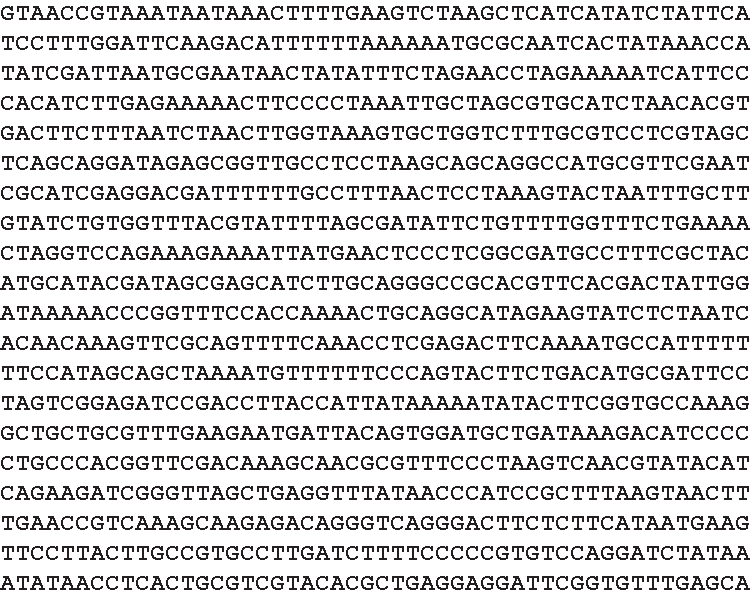
\includegraphics[width=10.8425in]{figs/genome-1kb-black}}
\center{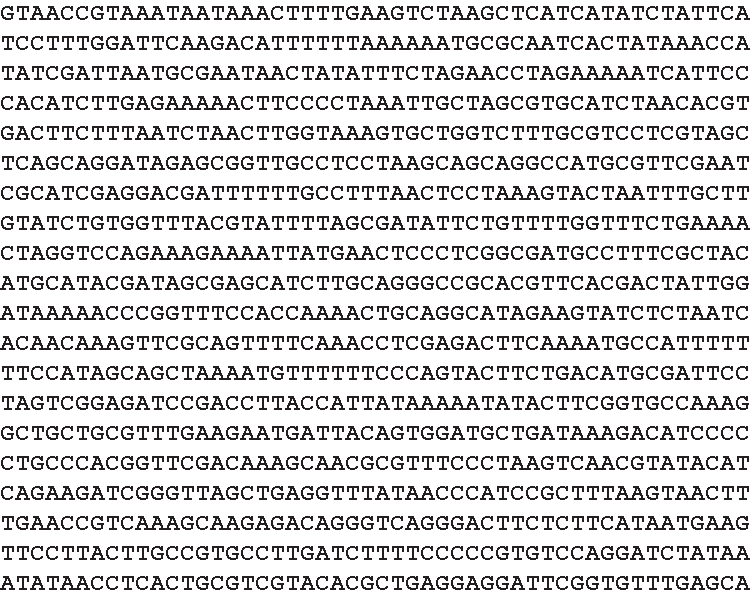
\includegraphics[height=8.34in]{figs/genome-1kb-black}}
\end{slide}
%%%%%%%%%%%%%%%%%%%%%%%%%%%%%%%%%%%%%%%%%%%%%%%%%%%%%%%%%%%%%%%%%%%%
\begin{slide}
\center{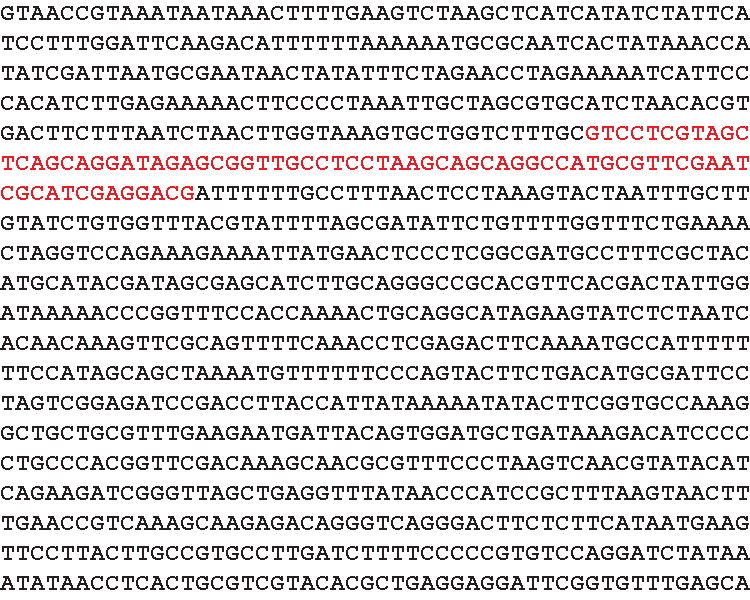
\includegraphics[height=8.34in]{figs/genome-1kb}}
\end{slide}
%%%%%%%%%%%%%%%%%%%%%%%%%%%%%%%%%%%%%%%%%%%%%%%%%%%%%%%%%%%%%%%%%%%%
\begin{comment}
\begin{slide}
\center{
\includegraphics[height=8.34in]{figs/genome-10kb}}
\end{slide}
\end{comment}
%%%%%%%%%%%%%%%%%%%%%%%%%%%%%%%%%%%%%%%%%%%%%%%%%%%%%%%%%%%%%%%%%%%%
\begin{slide}
\center{
\includegraphics[height=8.34in]{figs/genome-100kb}}
\end{slide}
%%%%%%%%%%%%%%%%%%%%%%%%%%%%%%%%%%%%%%%%%%%%%%%%%%%%%%%%%%%%%%%%%%%%
\begin{comment}
\begin{slide}
\center{\includegraphics[height=8.34in]{figs/genome-full}}
\end{slide}
\end{comment}
%%%%%%%%%%%%%%%%%%%%%%%%%%%%%%%%%%%%%%%%%%%%%%%%%%%%%%%%%%%%%%%%%%%%
\begin{slide}
\begin{center}
\textbf{Identifying functional sequences in genomes \\
  is a fundamental problem in computational biology.}
\end{center}
\medskip

\begin{center}
\begin{tabular}{ll}
Protein-coding genes: & DNA $\rightarrow$ mRNA $\rightarrow$ protein \\
& \\
\textcolor{red}{Functional RNA genes:} & \textcolor{red}{DNA  $\rightarrow$ RNA} \\
& \\
Transcription factor binding sites & \\
& \\
Enhancers & \\
\end{tabular}
\end{center}

\vfill
\end{slide}
%%%%%%%%%%%%%%%%%%%%%%%%%%%%%%%%%%%%%%%%%%%%%%%%%%%%%%%%%%%%%%%%%%%%
\begin{slide}
\begin{center}
\textbf{Identifying functional sequences in genomes \\
  is a fundamental problem in computational biology.}
\end{center}
\medskip

\begin{center}
\begin{tabular}{ll}
Protein-coding genes: & DNA $\rightarrow$ mRNA $\rightarrow$ protein \\
& \\
\textcolor{red}{Functional RNA genes:} & \textcolor{red}{DNA  $\rightarrow$ RNA} \\
& \\
Transcription factor binding sites & \\
& \\
Enhancers & \\
\end{tabular}
\medskip

\medskip

\medskip

\medskip

\textbf{How can we find functional sequences?}

{\bf By searching for similarity with known genes \\
indicative of shared evolutionary history}

\begin{tabular}{rl}
Gene family: & group of evolutionarily related ({\em homologous}) \\
& genes in different genomes \\
& \\
Homology search: & given one or more homologs of a \\
& family, find more \\
\end{tabular}

%{\bf Gene \emph{function} is evolutionarily conserved, which means
%  functionally important structure and sequence features are too.}

%{\bf Functionally important sequence features are \\ evolutionarily conserved in
%  homologs.}

%{\bf Homologous genes often share similar \\ functions, structures and
%  sequences}

\end{center}

\vfill
\end{slide}
%%%%%%%%%%%%%%%%%%%%%%%%%%%%%%%%%%%%%%%%%%%%%%%%%%%%%%%%%%%%%%%
\begin{slide}
\begin{center}
{\bf Most proteins and RNAs adopt a conserved 3-dimensional 
  structure that is responsible for their function in the cell}

\medskip

Three representations of a transfer RNA:

%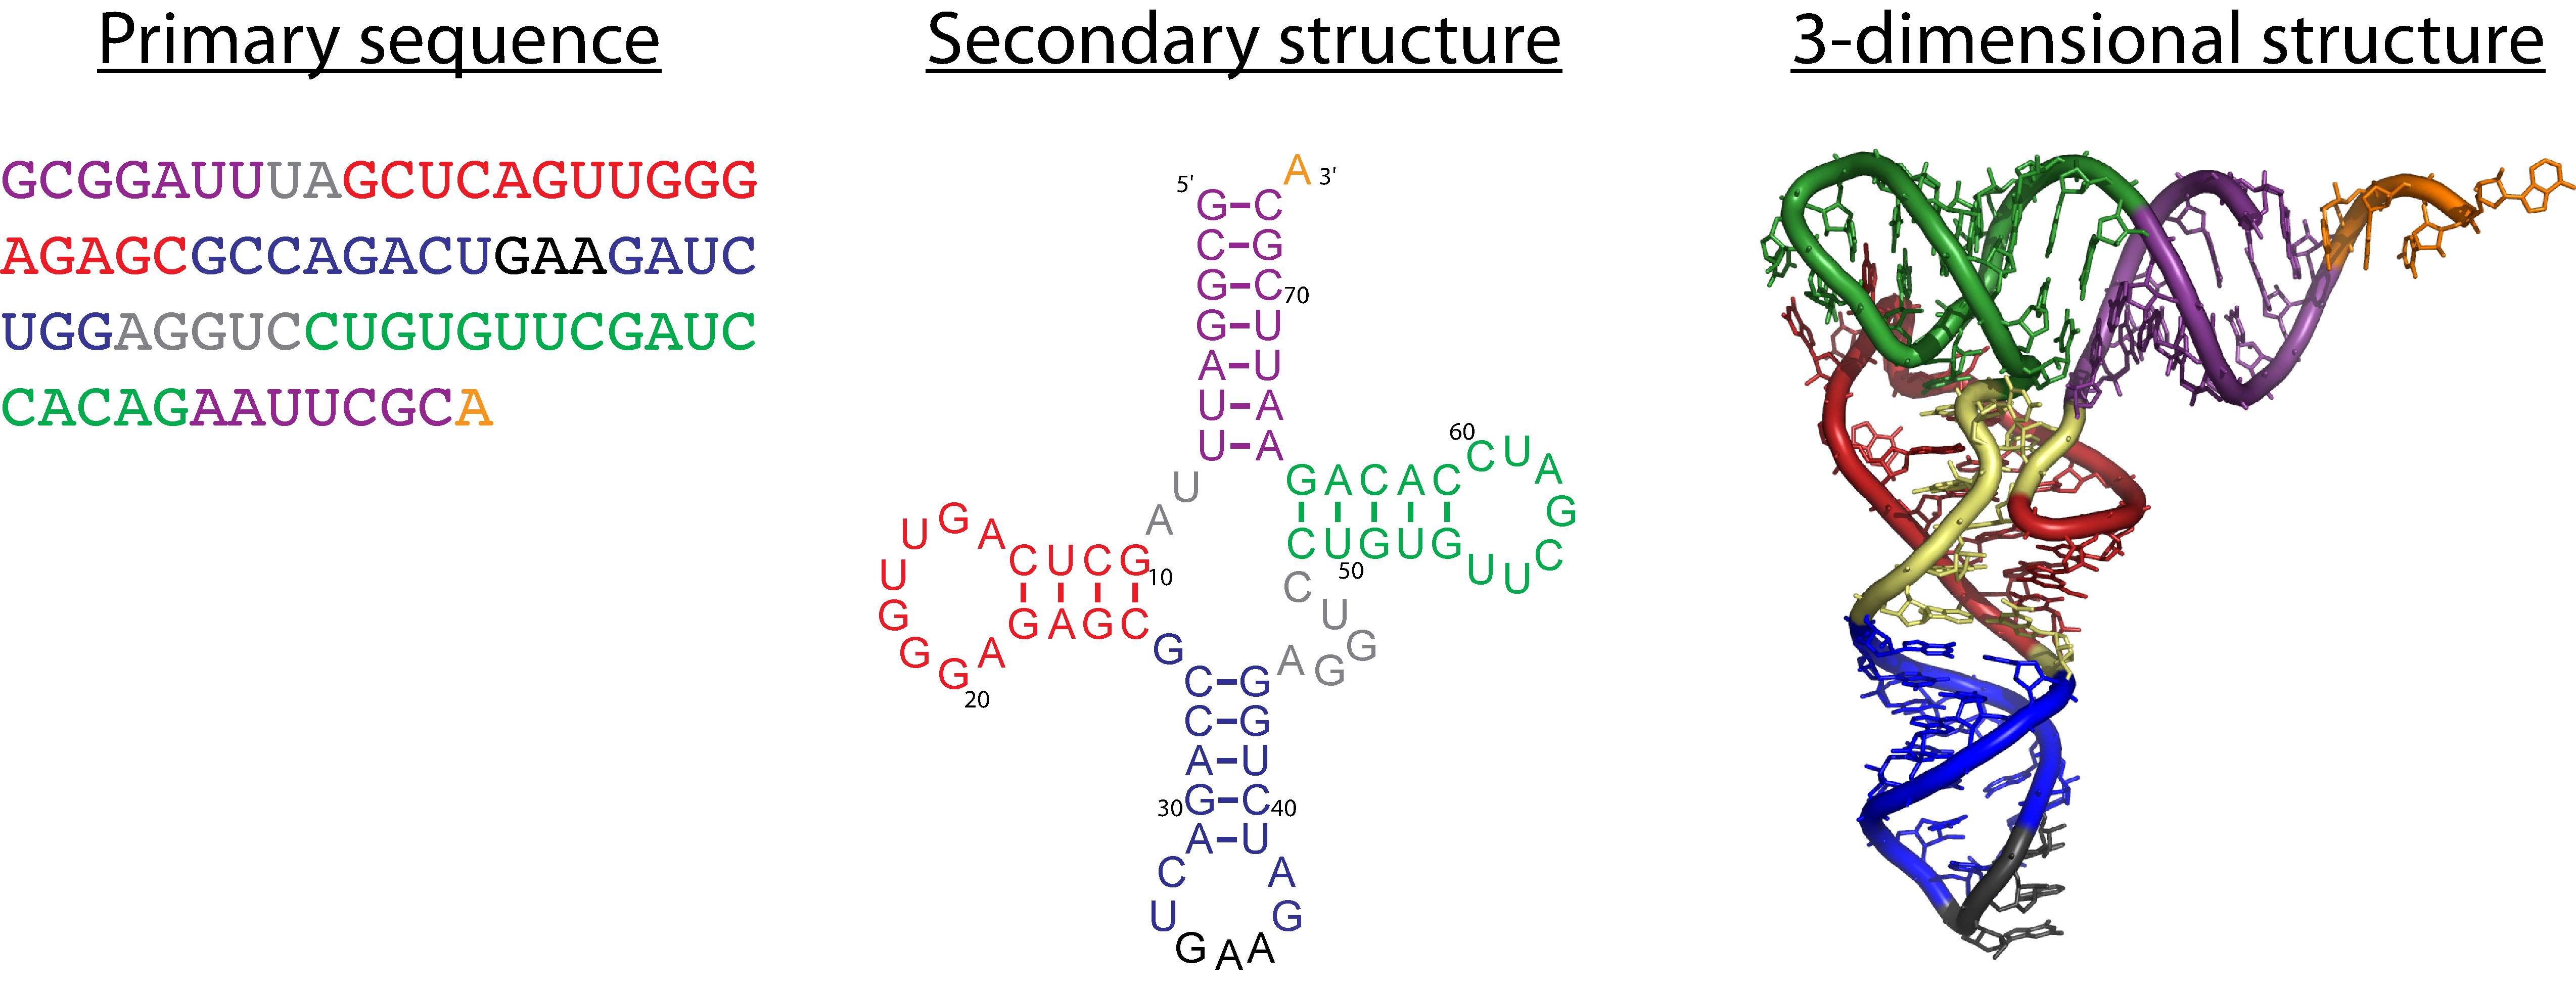
\includegraphics[width=10.5in]{figs/trna-123}
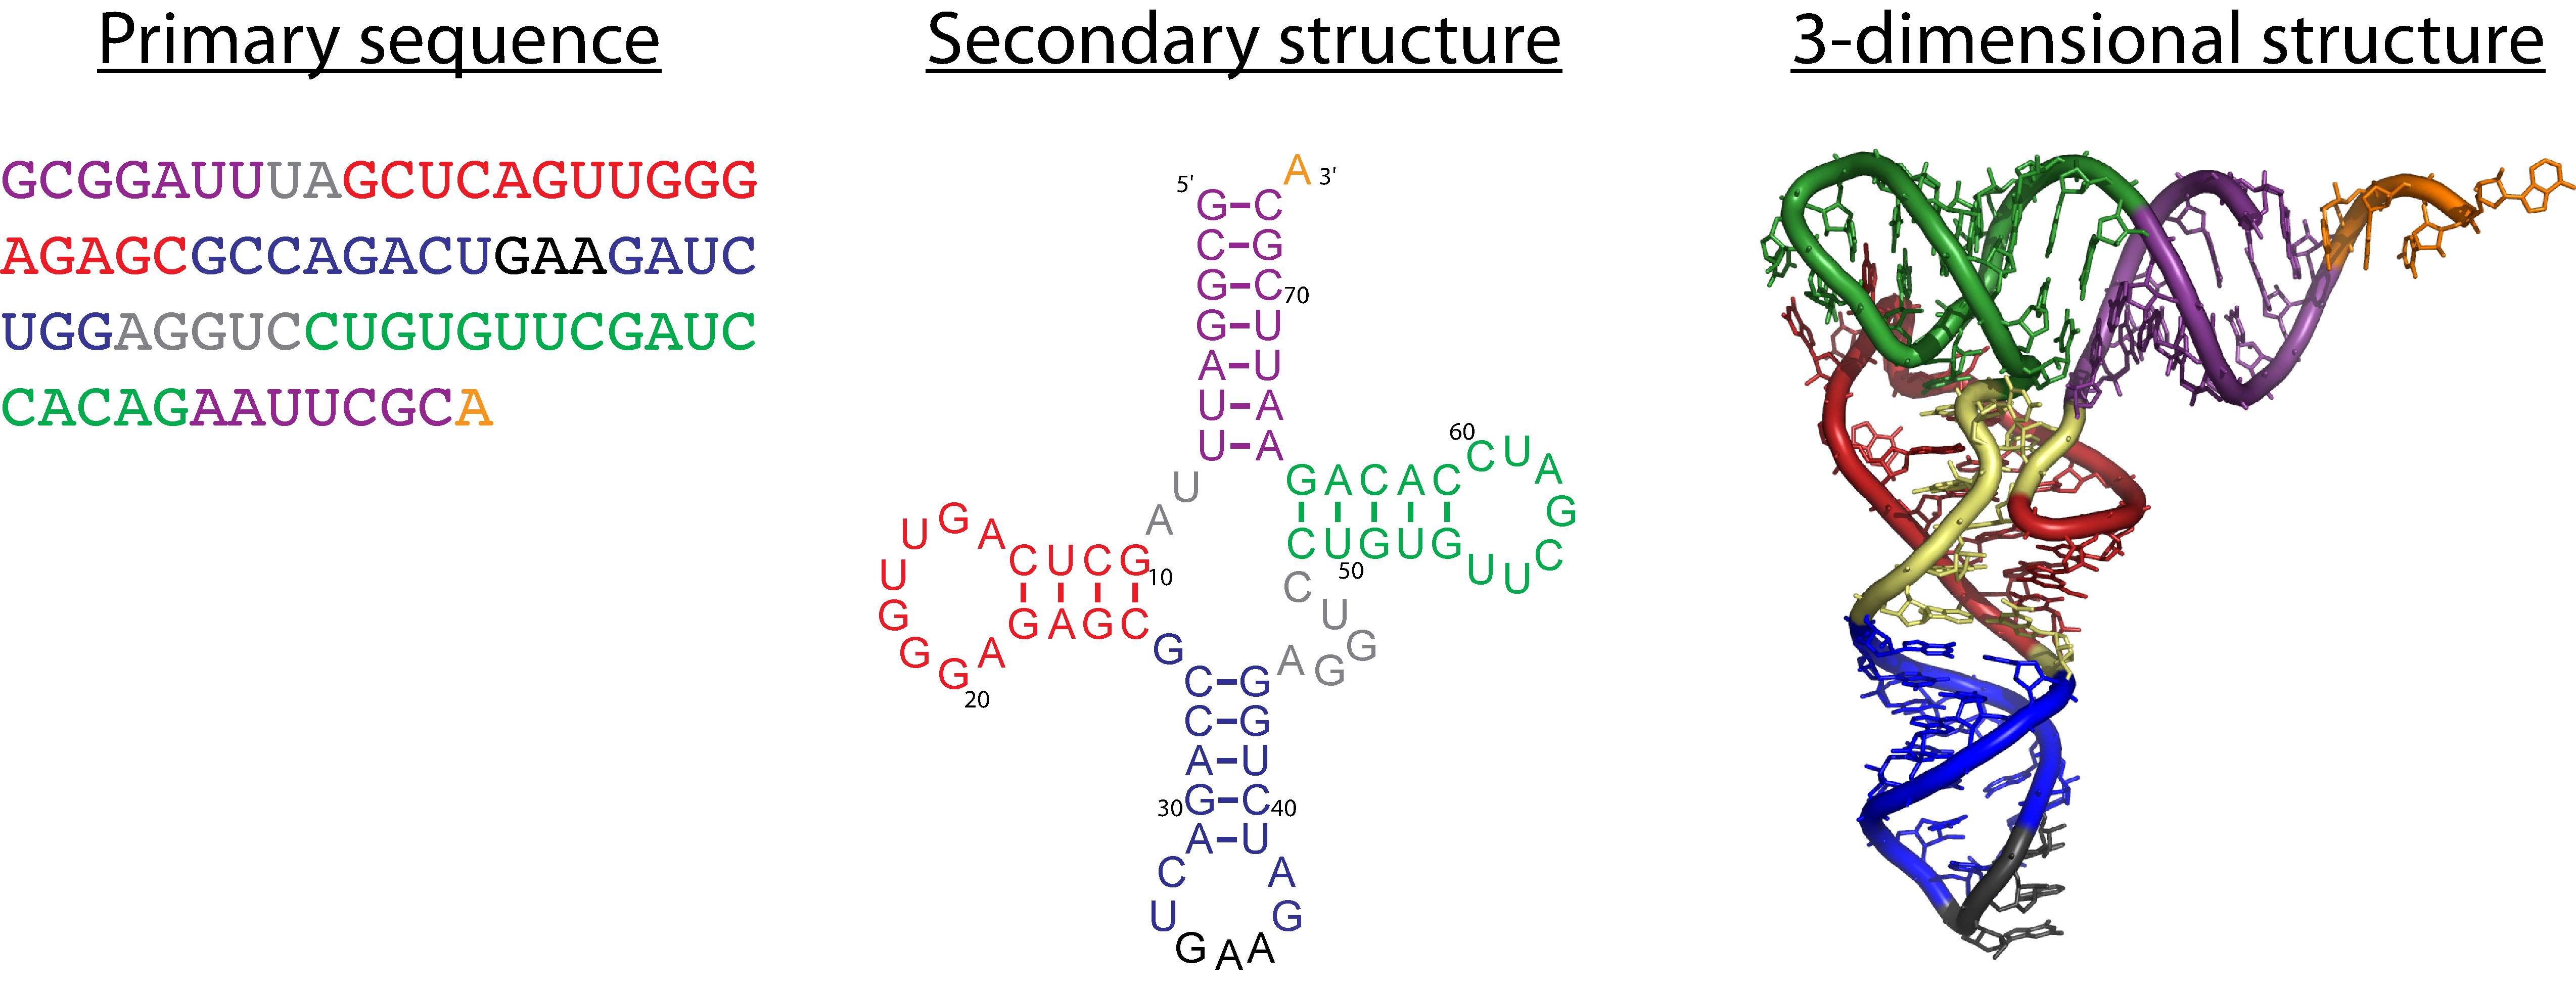
\includegraphics[width=9in]{figs/trna-123}

\end{center}

\vfill

\end{slide}
%%%%%%%%%%%%%%%%%%%%%%%%%%%%%%%%%%%%%%%%%%%%%%%%%%%%%%%%%%%%%%
\begin{slide}
\begin{center}
{\bf Most proteins and RNAs adopt a conserved 3-dimensional 
  structure that is responsible for their function in the cell}

\medskip

Three representations of a transfer RNA:

%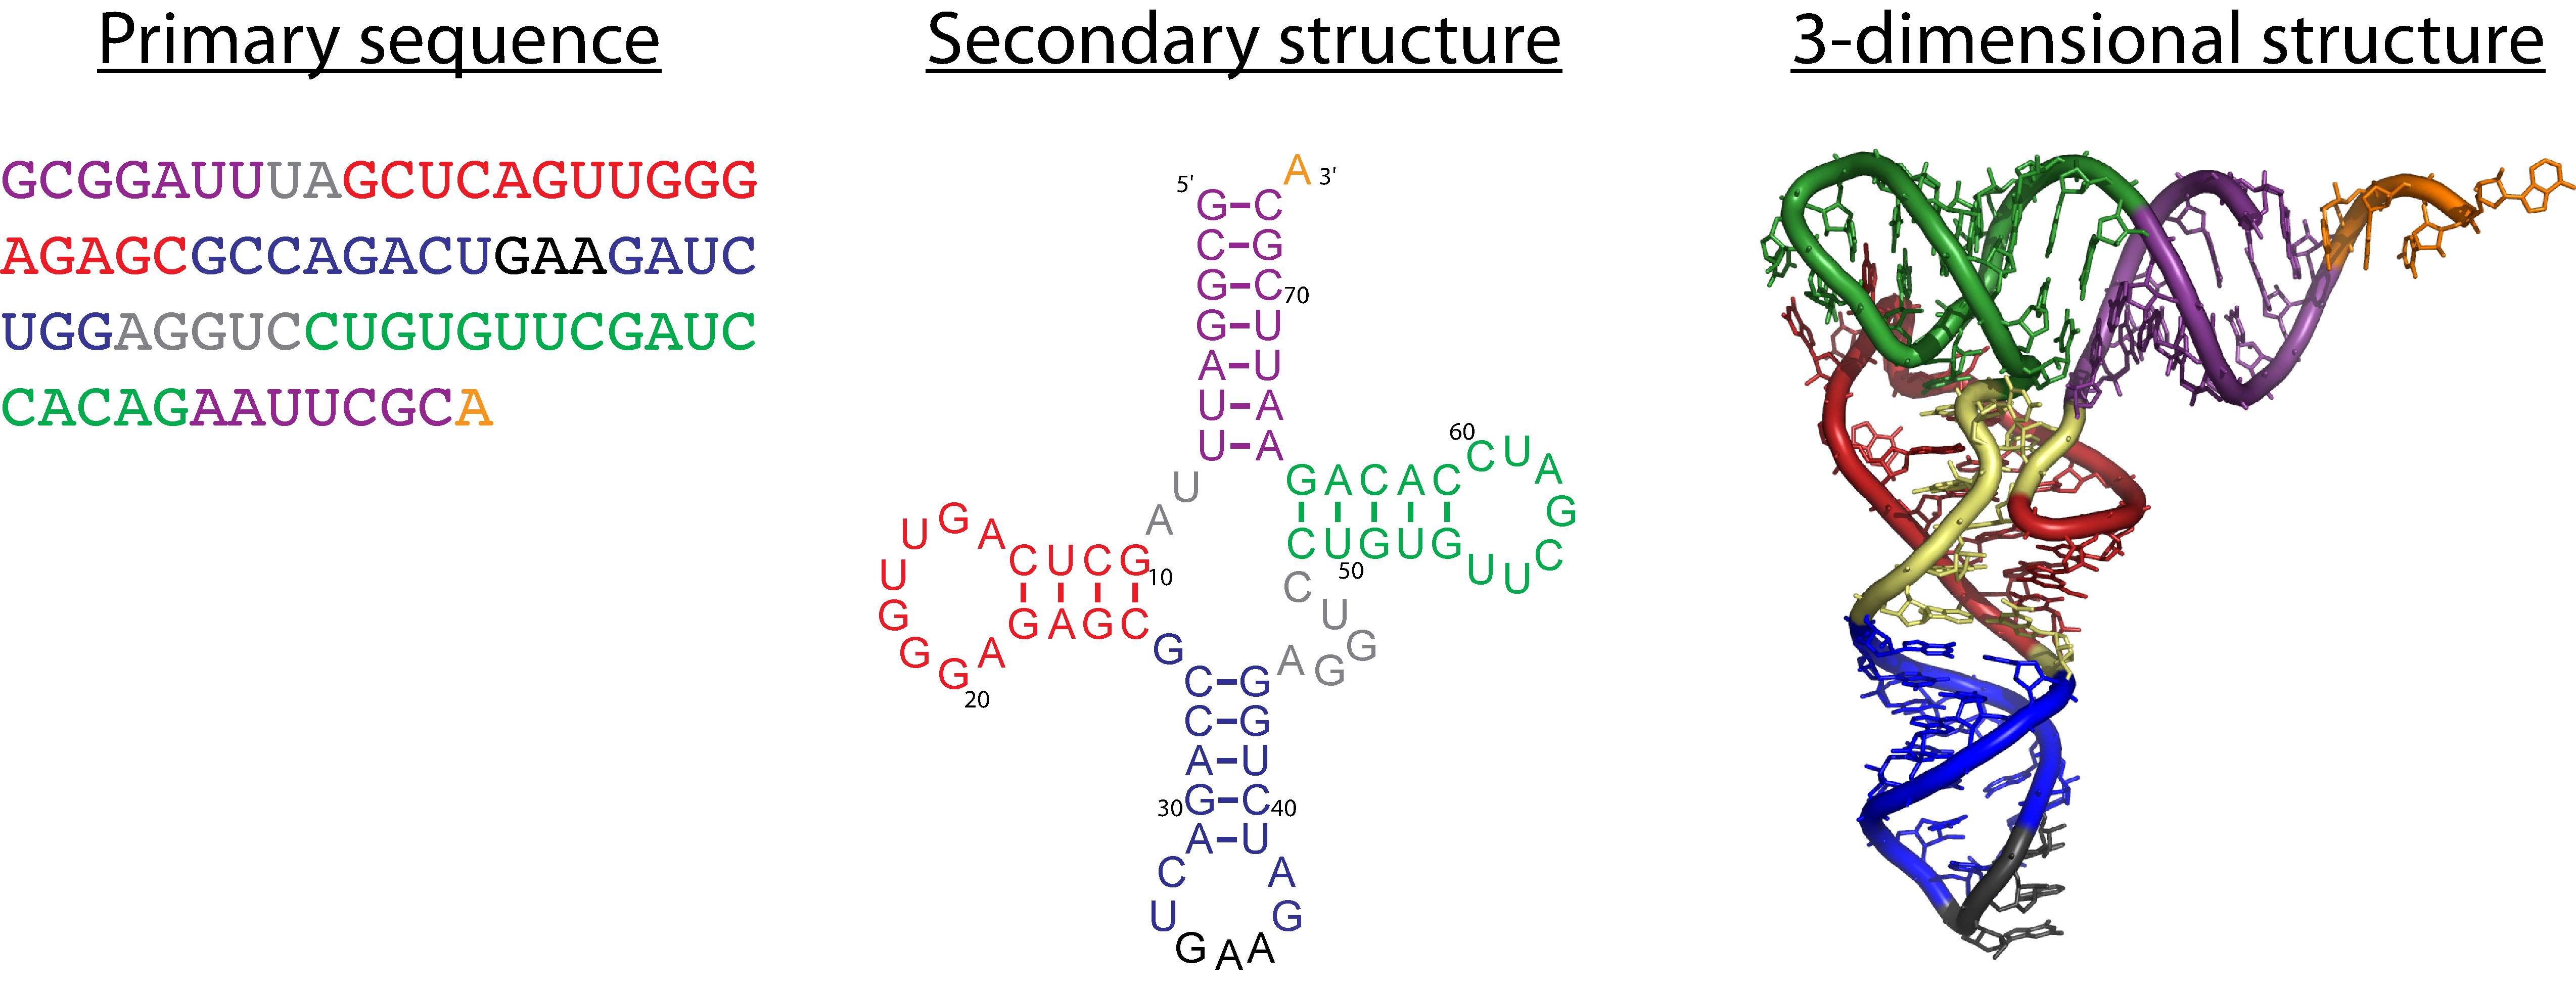
\includegraphics[width=10.5in]{figs/trna-123}
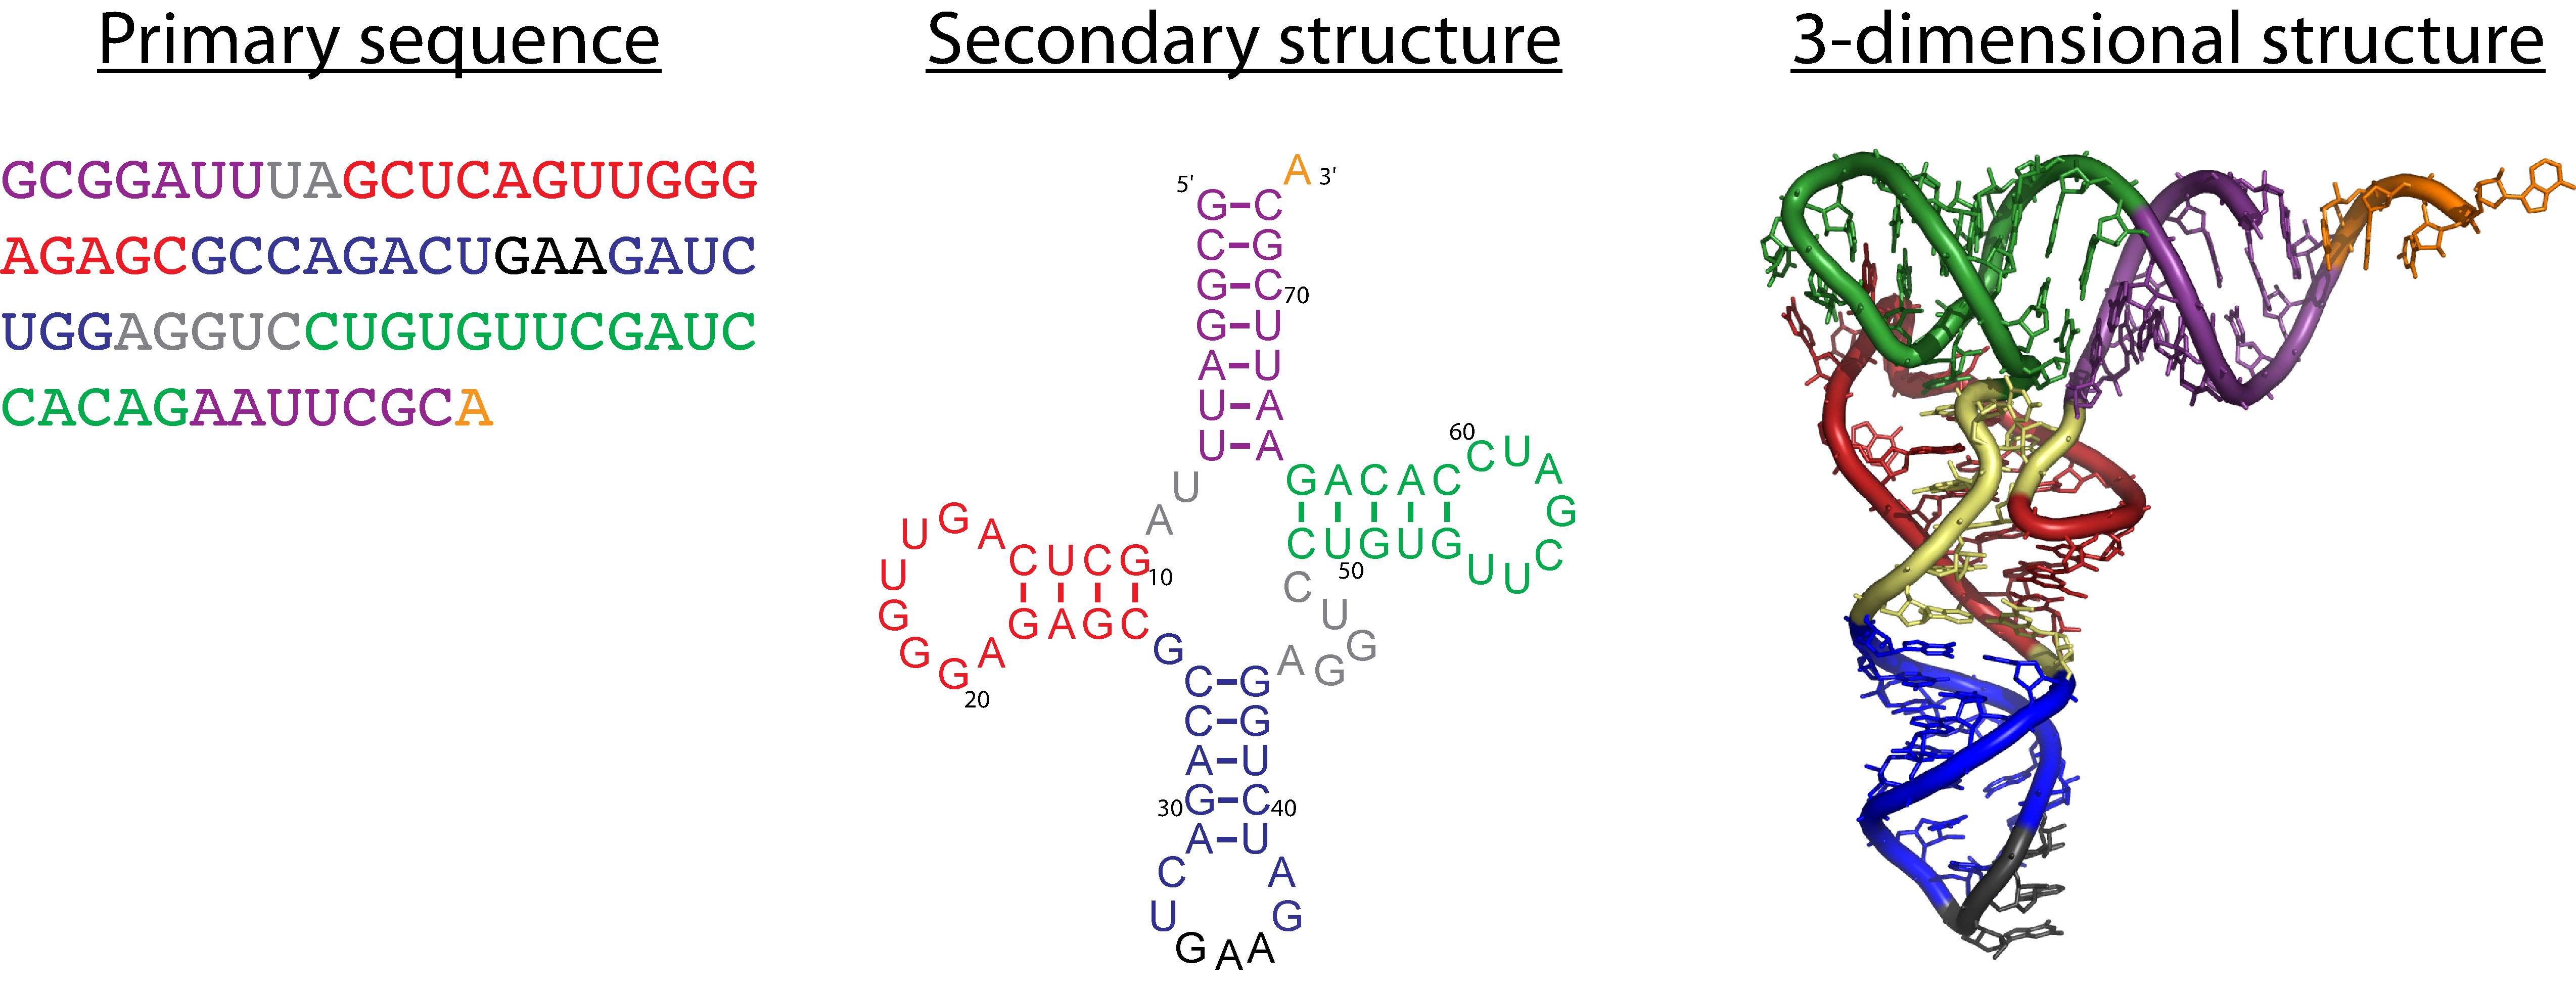
\includegraphics[width=9in]{figs/trna-123}

{\bf BLAST:} given a single sequence, search genomes for similar sequences.

%{\bf Homologous proteins and RNAs conserve \\ both sequence
%and structural features}

{\bf Homologous proteins and RNAs conserve different sequence \\
and structural features to different degrees.}
\end{center}

\vfill

\end{slide}
%%%%%%%%%%%%%%%%%%%%%%%%%%%%%%%%%%%%%%%%%%%%%%%%%%%%%%%%%%%%%
\begin{slide}
\begin{center}
%\textbf{Comparative analysis of sequence families}: \\
\textbf{Sequence conservation provides \\ information for homology searches}
%\emph{Functionally important sequence features are evolutionarily conserved.}
\medskip

%A simple, made-up RNA family:

%Evolution conserves functionally \\ important sequence features.

%Evolution conserves sequence \\ based on its functional importance.

Conservation levels vary across alignment columns.

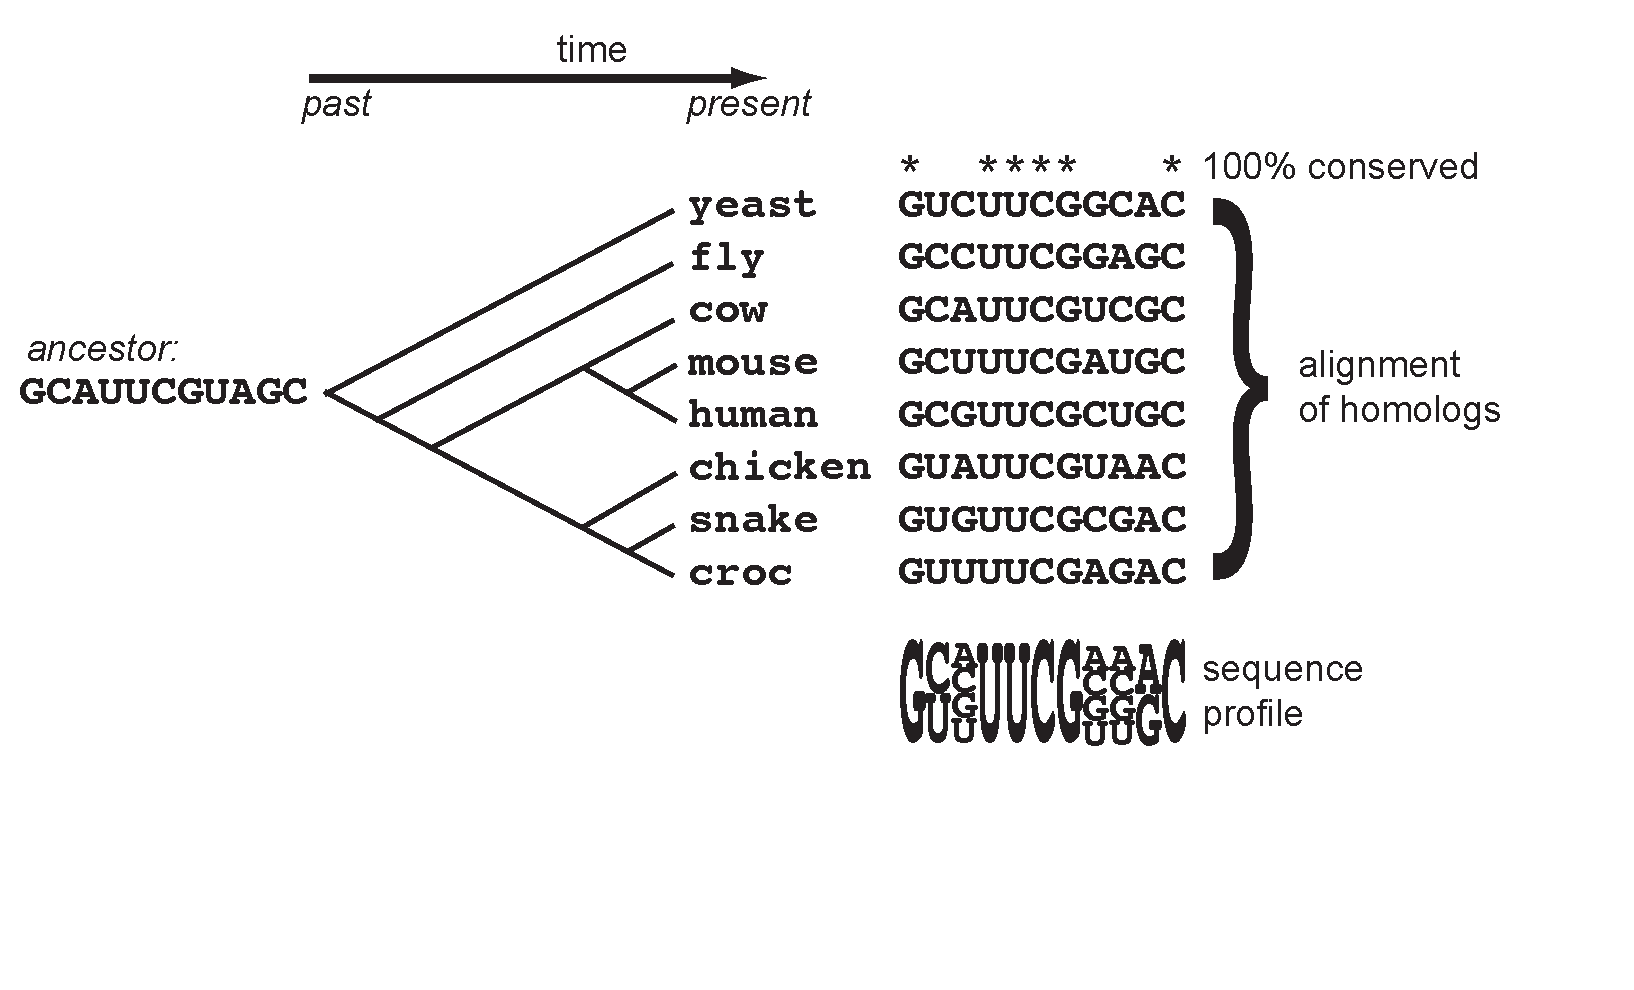
\includegraphics[width=10in]{figs/seqstructprofiles-seq1}
\end{center}

\vfill
\end{slide}
%%%%%%%%%%%%%%%%%%%%%%%%%%%%%%%%%%%%%%%%%%%%%%%%%%%%%%%%%%%%%%%%%%%%%%
\begin{slide}
\begin{center}
\textbf{Structure conservation provides additional information}
\medskip

Base-paired positions covary \\ to maintain Watson-Crick complementarity.

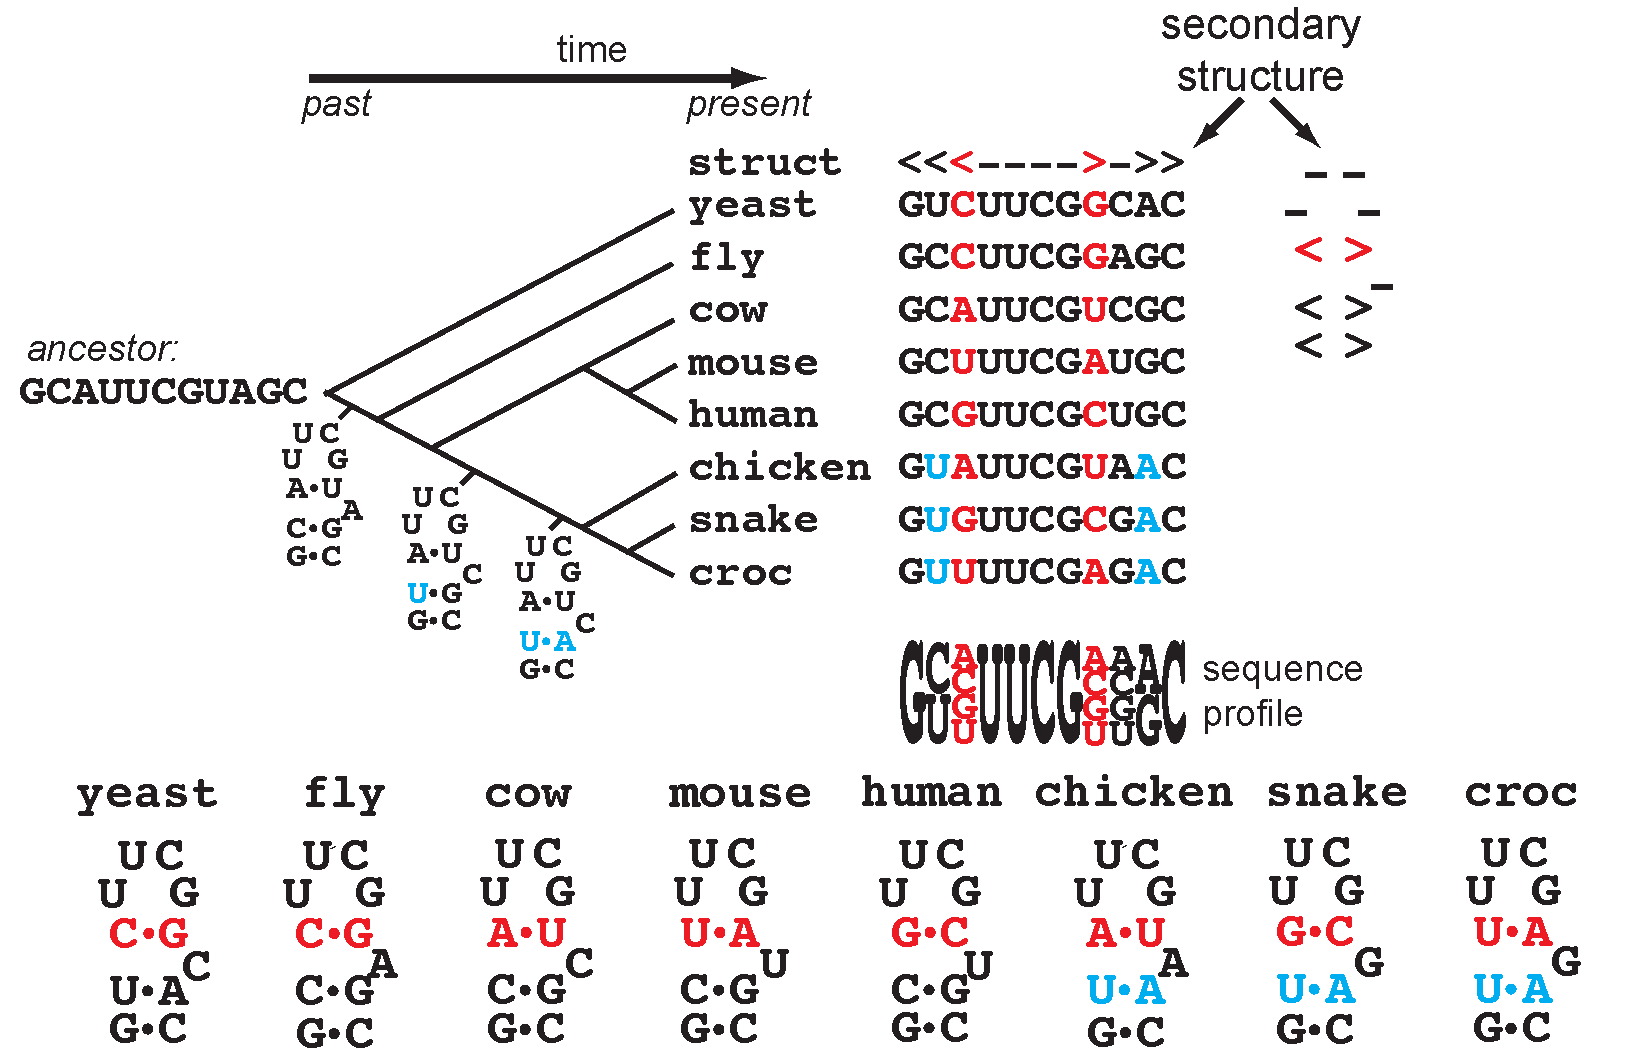
\includegraphics[width=10in]{figs/seqstructprofiles-struct2}
\end{center}

\vfill
\end{slide}
%%%%%%%%%%%%%%%%%%%%%%%%%%%%%%%%%%%%%%%%%%%%%%%%%%%%%%%%%%%%%%%%%%%%%%%%%%
\begin{slide}
\begin{center}
\textbf{Amount of information in a profile can be measured in bits}
\medskip

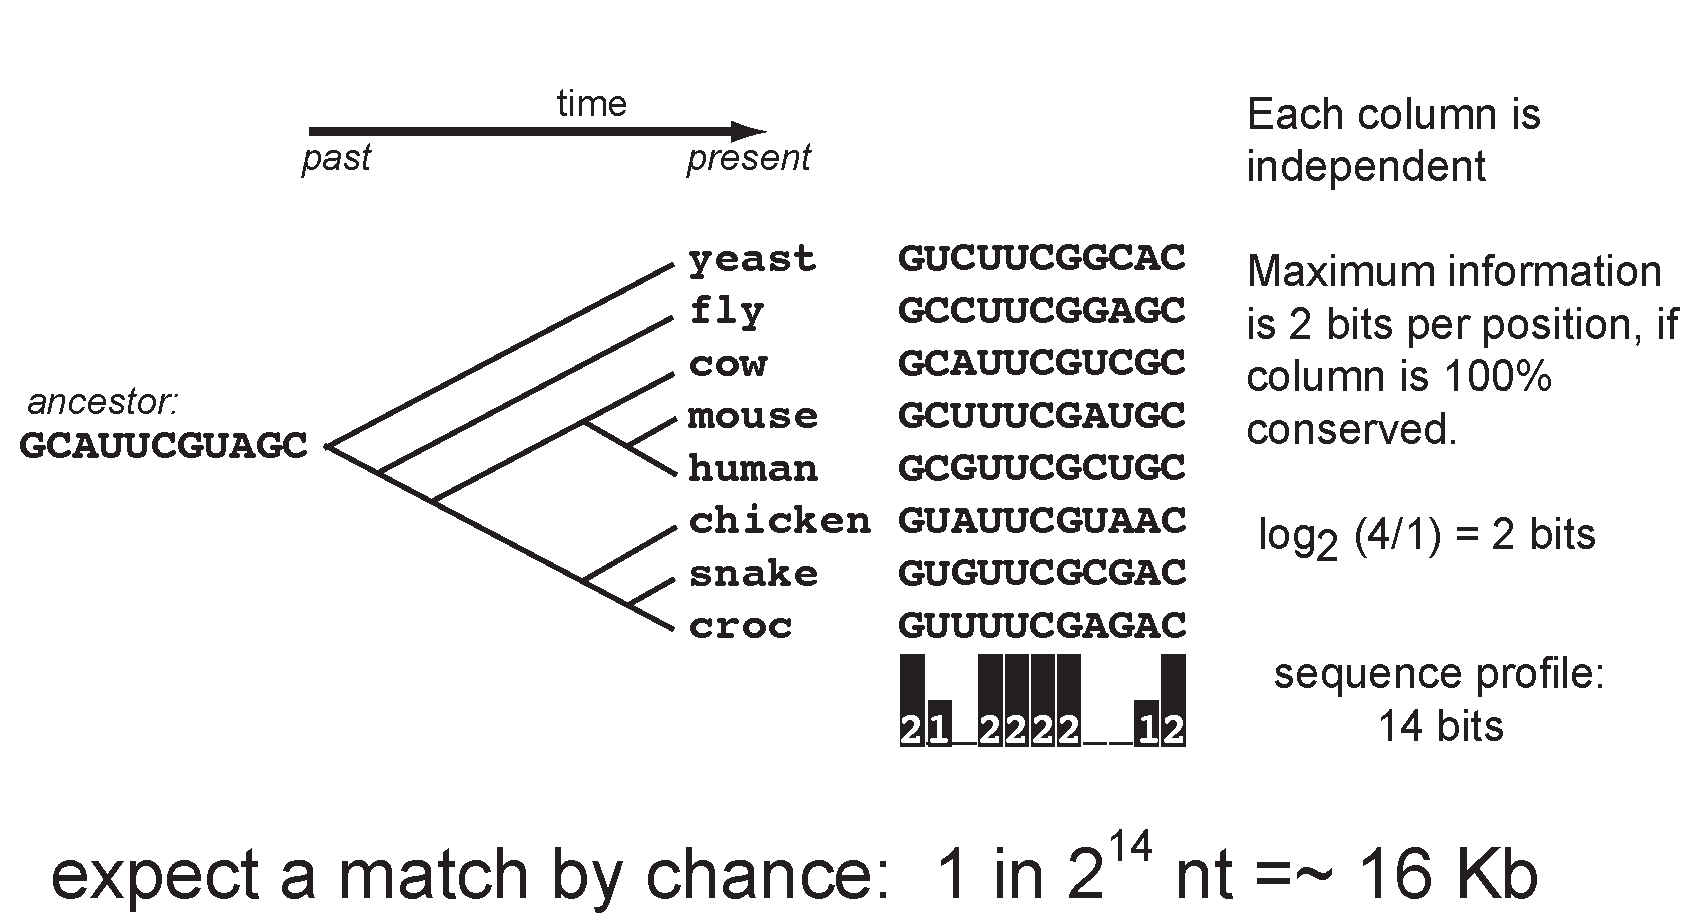
\includegraphics[width=9in]{figs/seqstructprofiles-2014-seqinfo}
\end{center}

\vfill
\end{slide}
%%%%%%%%%%%%%%%%%%%%%%%%%%%%%%%%%%%%%%%%%%%%%%%%%%%%%%%%%%%%%%%%%%%%%%%%%%
\begin{slide}
\begin{center}
\textbf{Structure contributes additional information from covariation}
\medskip

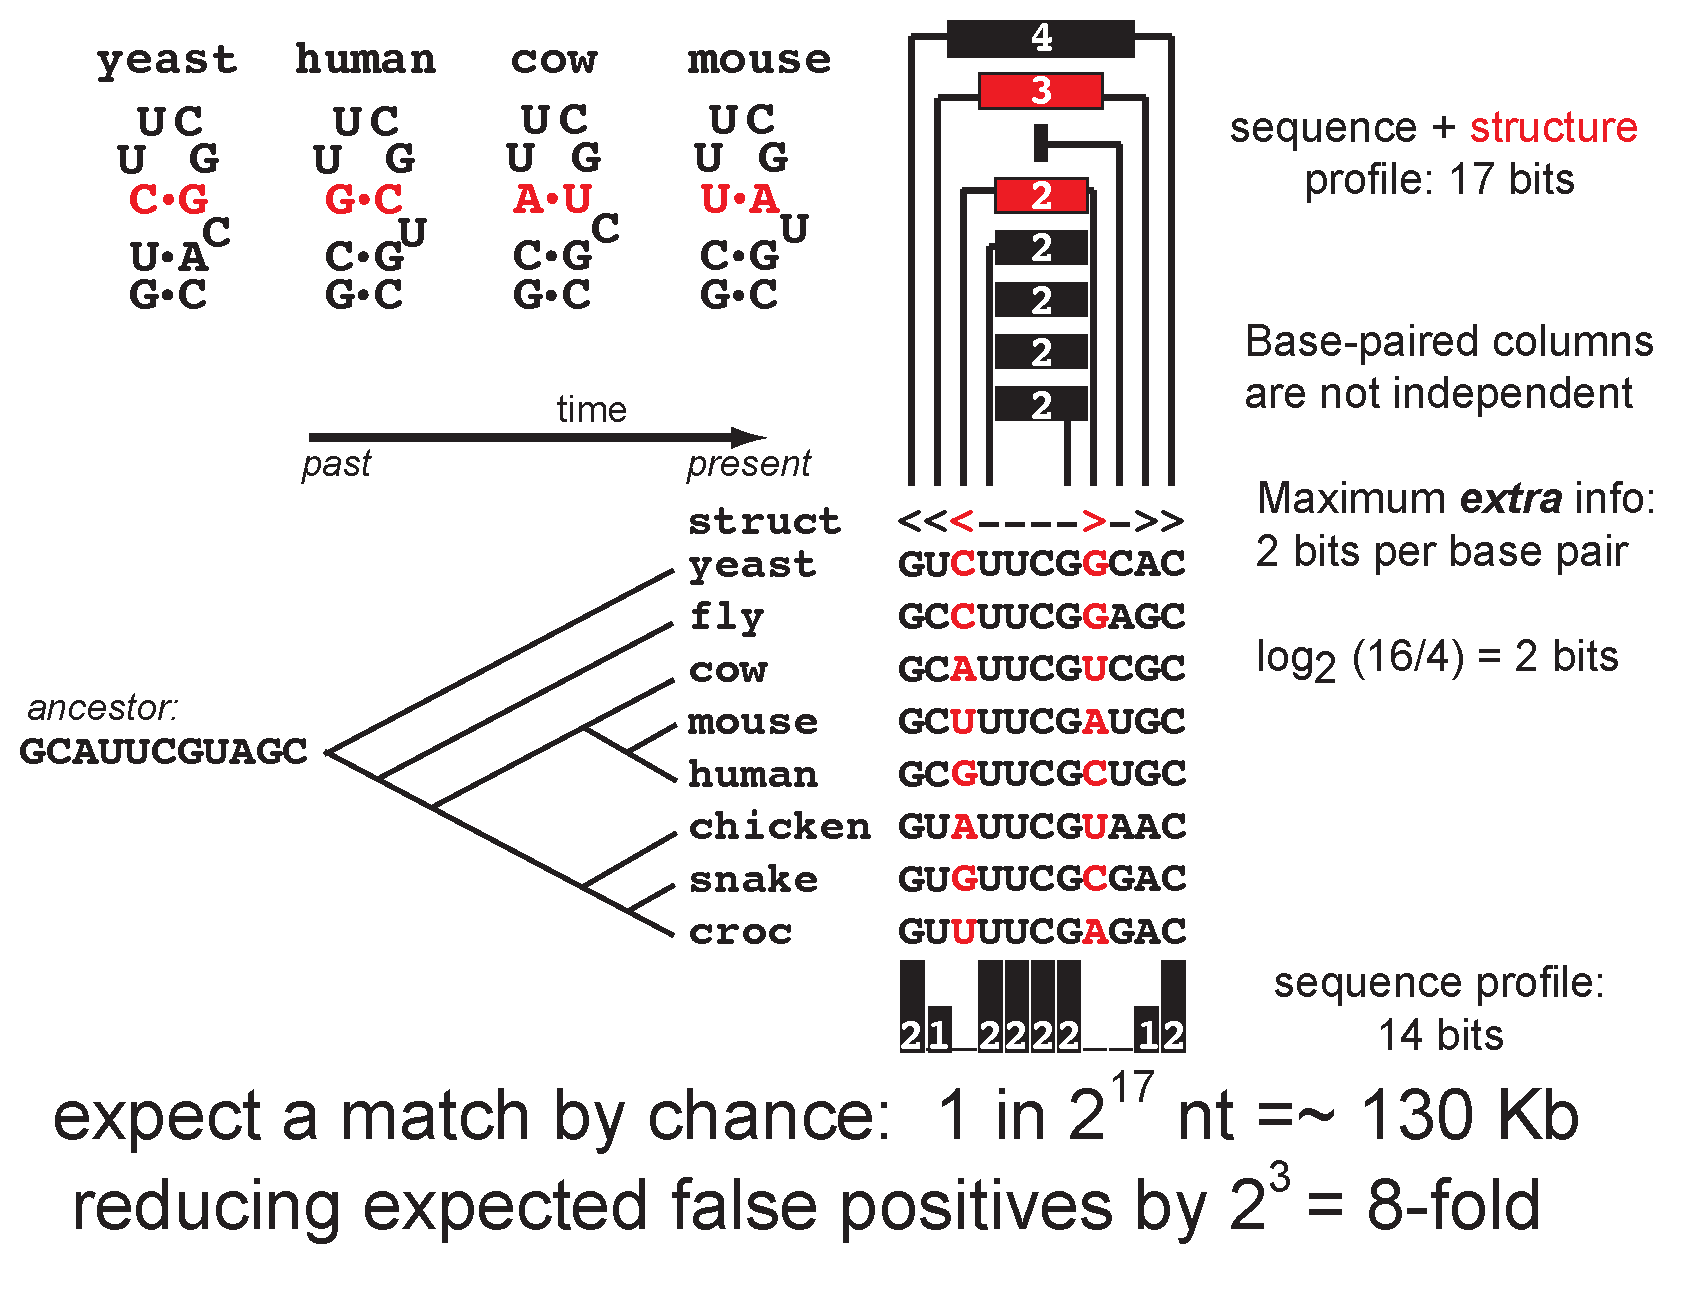
\includegraphics[width=9in]{figs/seqstructprofiles-2014-structinfo}
\end{center}

\vfill
\end{slide}
%%%%%%%%%%%%%%%%%%%%%%%%%%%%%%%%%%%%%%%%%%%%%%%%%%%%%%%%%%%%%%%%%%%%%%%%%%
\begin{slide}
\begin{center}
\textbf{Levels of sequence and structure conservation in RNA families}
\end{center}
\medskip

\begin{center}
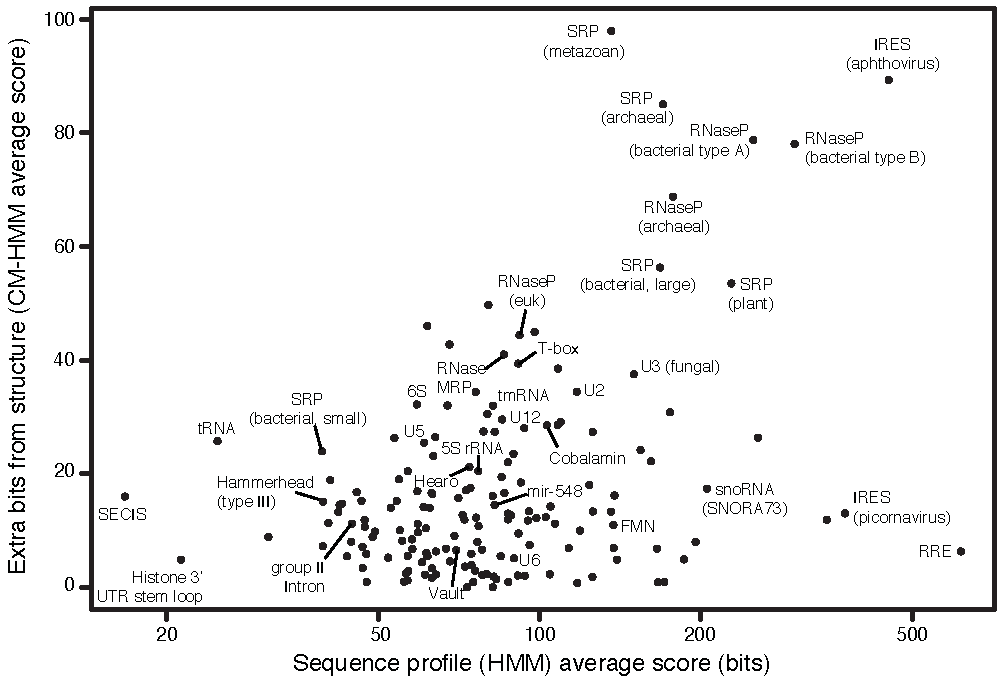
\includegraphics[height=6.5in]{figs/avgscores-rfam11}
\end{center}

\vfill

\end{slide}
%%%%%%%%%%%%%%%%%%%%%%%%%%%%%%%%%%%%%%%%%%%%%%%%%%%%%%%%%%%%%%%%%%%
\begin{slide}
\begin{center}
%\textbf{profile HMMs and covariance models}
\textbf{Eddy lab software for profile probabilistic models } (since 1994)
\end{center}
\medskip

\begin{center}
\small
\begin{tabular}{r|cc} 
%             &         & sequence \\
%             & sequence& and structure \\
%             & profiles& profiles \\ \hline
             & sequence & sequence and \\
             & profiles & structure profiles \\ \hline
  \\
  models     & profile HMMs     & {\color{red} covariance models (CMs)} \\ 
  \\
  software   & {\sc HMMER}      & {\sc Infernal} \\ 
  \\
  main use   & proteins         & RNAs \\ 
  \\
  database   & {\sc Pfam}       & {\sc Rfam} \\
             & (14831 families) & (2208 families) \\
  \\
%  primary sequence & yes & yes \\
%  \\
%  secondary structure & no & yes \\
%  \\
%  algorithms & Viterbi, Forward & CYK, Inside \\
%%             & Forward & Inside \\
%             &         & \\
%  complexity & $O(LN)$ & $O(LN^{2} log N)$ \\
%  \\
  performance& faster but    & slower but    \\
  for RNAs   & less accurate & more accurate \\
\end{tabular}

%\hspace{1.2in}
\includegraphics[height=2in]{figs/hmmer_logo}\hspace{1.05in}
\includegraphics[height=2.6in]{figs/infernal_logo}
\hspace{1.2in}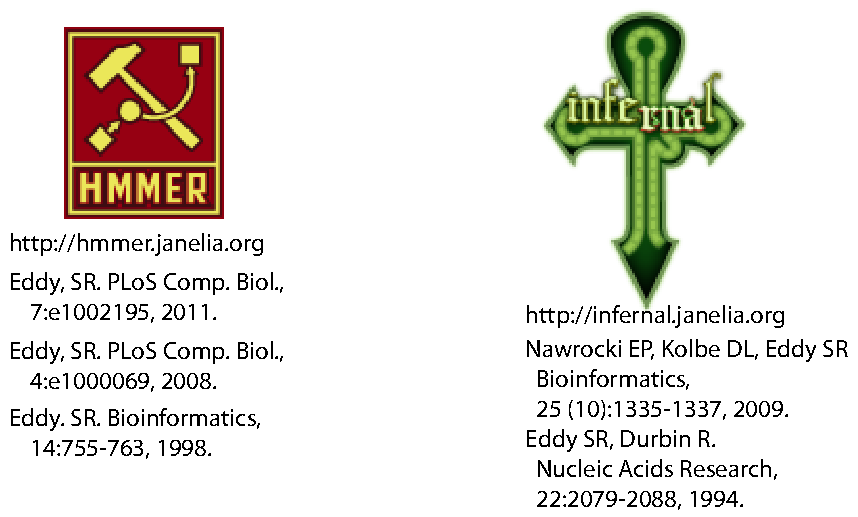
\includegraphics[height=2.7in]{figs/hmmer-infernal-refs}

\end{center}

\vfill

\end{slide}
%%%%%%%%%%%%%%%%%%%%%%%%%%%%%%%%%%%%%%%%%%%%%%%%%%%%%%%%%%%%%%%
%%%%%%%%%%%%%%%%%%%%%%%%%%%%%%%%%%%%%%%%%%%%%%%%%%%%%%%%%%%%%%%%%%%%
\begin{slide}
\begin{center}
%\textbf{profile HMMs and covariance models}
\textbf{Profile HMMs: sequence family models built from alignments}
\end{center}

\center{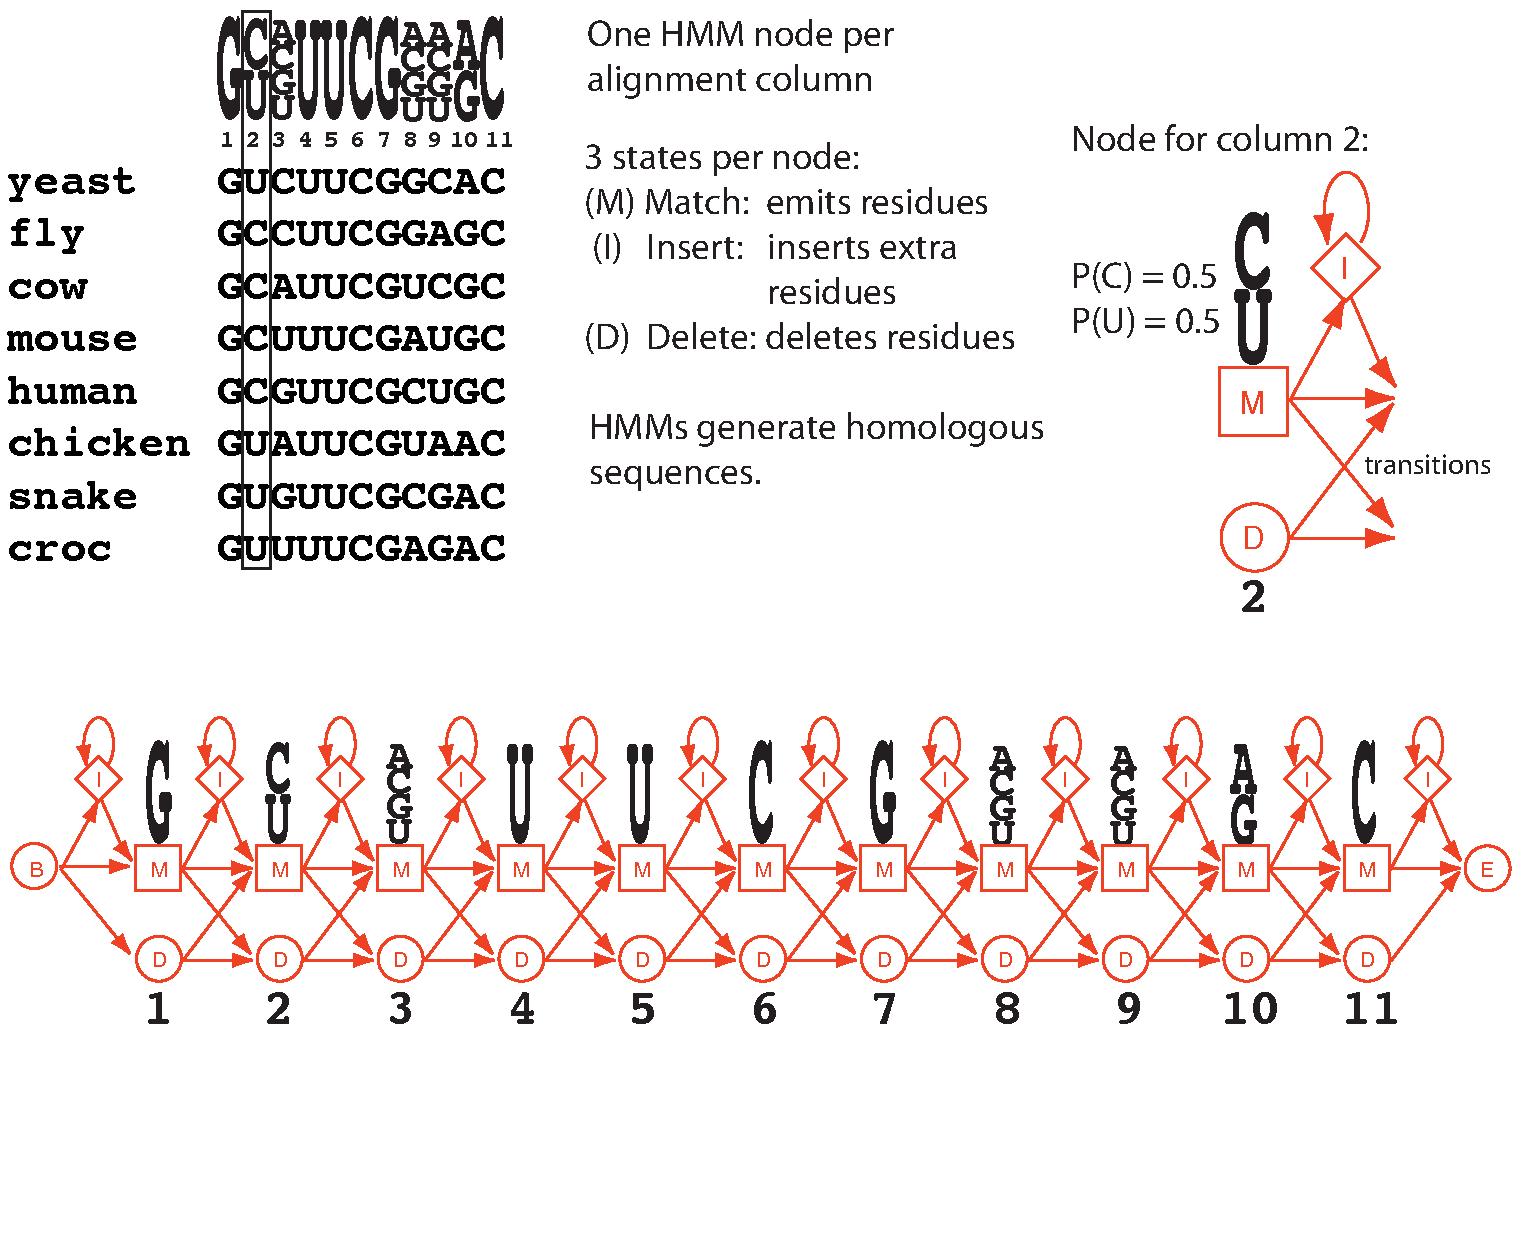
\includegraphics[height=6.625in]{figs/hmm}}

%An HMM generates ``homologous'' sequences.

\end{slide}
%%%%%%%%%%%%%%%%%%%%%%%%%%%%%%%%%%%%%%%%%%%%%%%%%%%%%%%%%%%%%%%
\begin{slide}
\begin{center}
%\textbf{profile HMMs and covariance models}
\textbf{Profile HMMs: sequence family models built from alignments}
\end{center}

\center{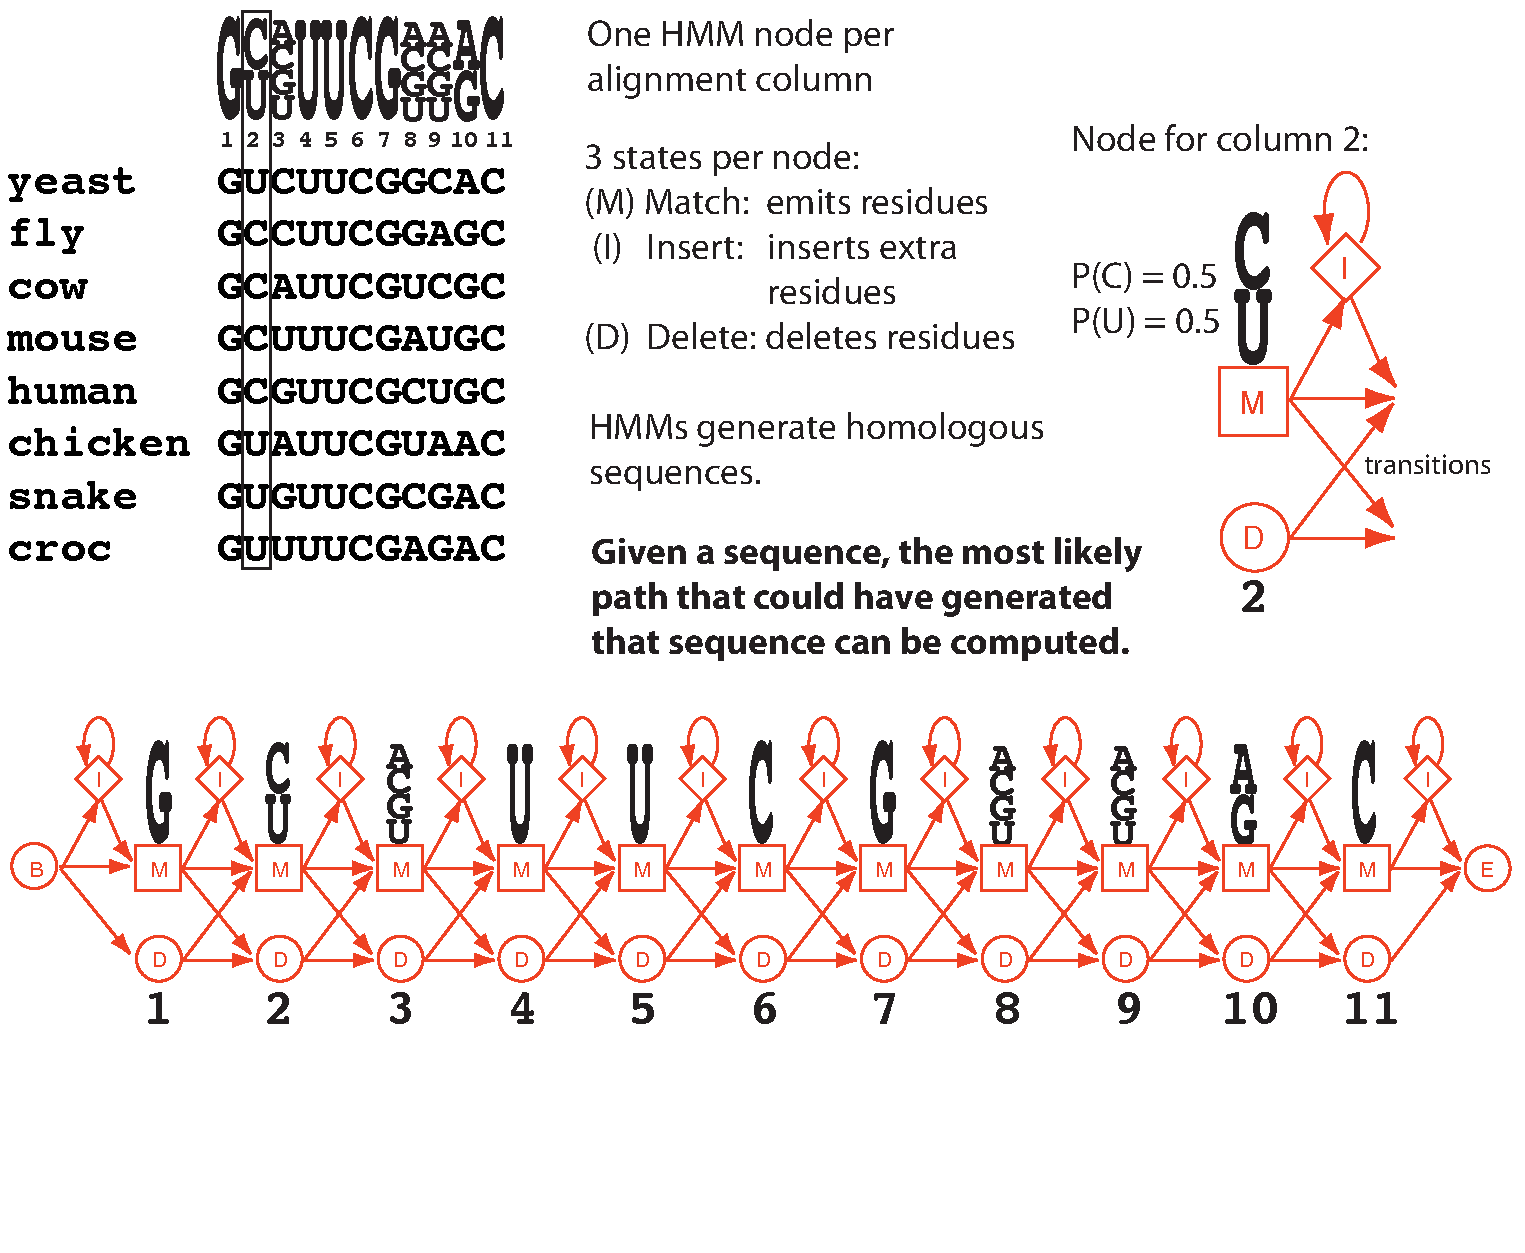
\includegraphics[height=6.625in]{figs/hmm-given}}
\end{slide}
%%%%%%%%%%%%%%%%%%%%%%%%%%%%%%%%%%%%%%%%%%%%%%%%%%%%%%%%%%%%%%%
\begin{slide}
\begin{center}
%\textbf{profile HMMs and covariance models}
\textbf{Profile HMMs: sequence family models built from alignments}
\end{center}

\center{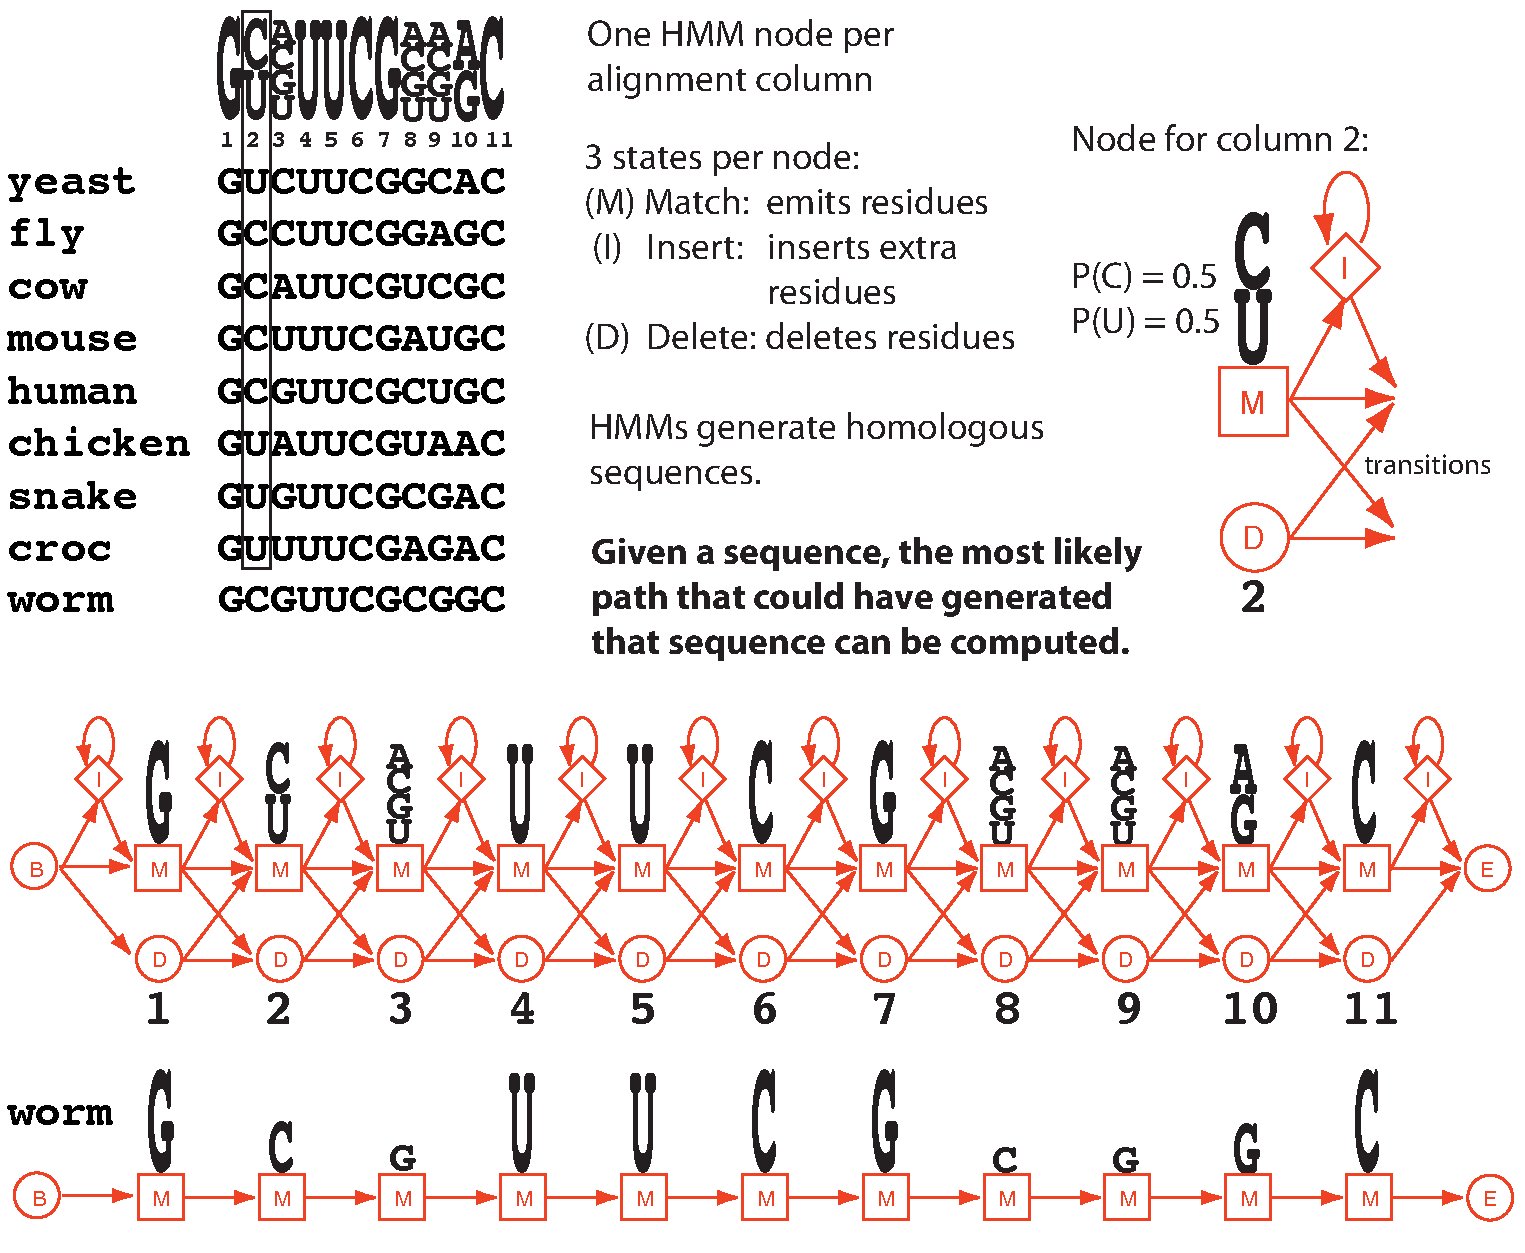
\includegraphics[height=6.625in]{figs/hmm-worm}}
\end{slide}
%%%%%%%%%%%%%%%%%%%%%%%%%%%%%%%%%%%%%%%%%%%%%%%%%%%%%%%%%%%
\begin{slide}
\begin{center}
%\textbf{profile HMMs and covariance models}
\textbf{Profile HMMs: sequence family models built from alignments}
\end{center}

\center{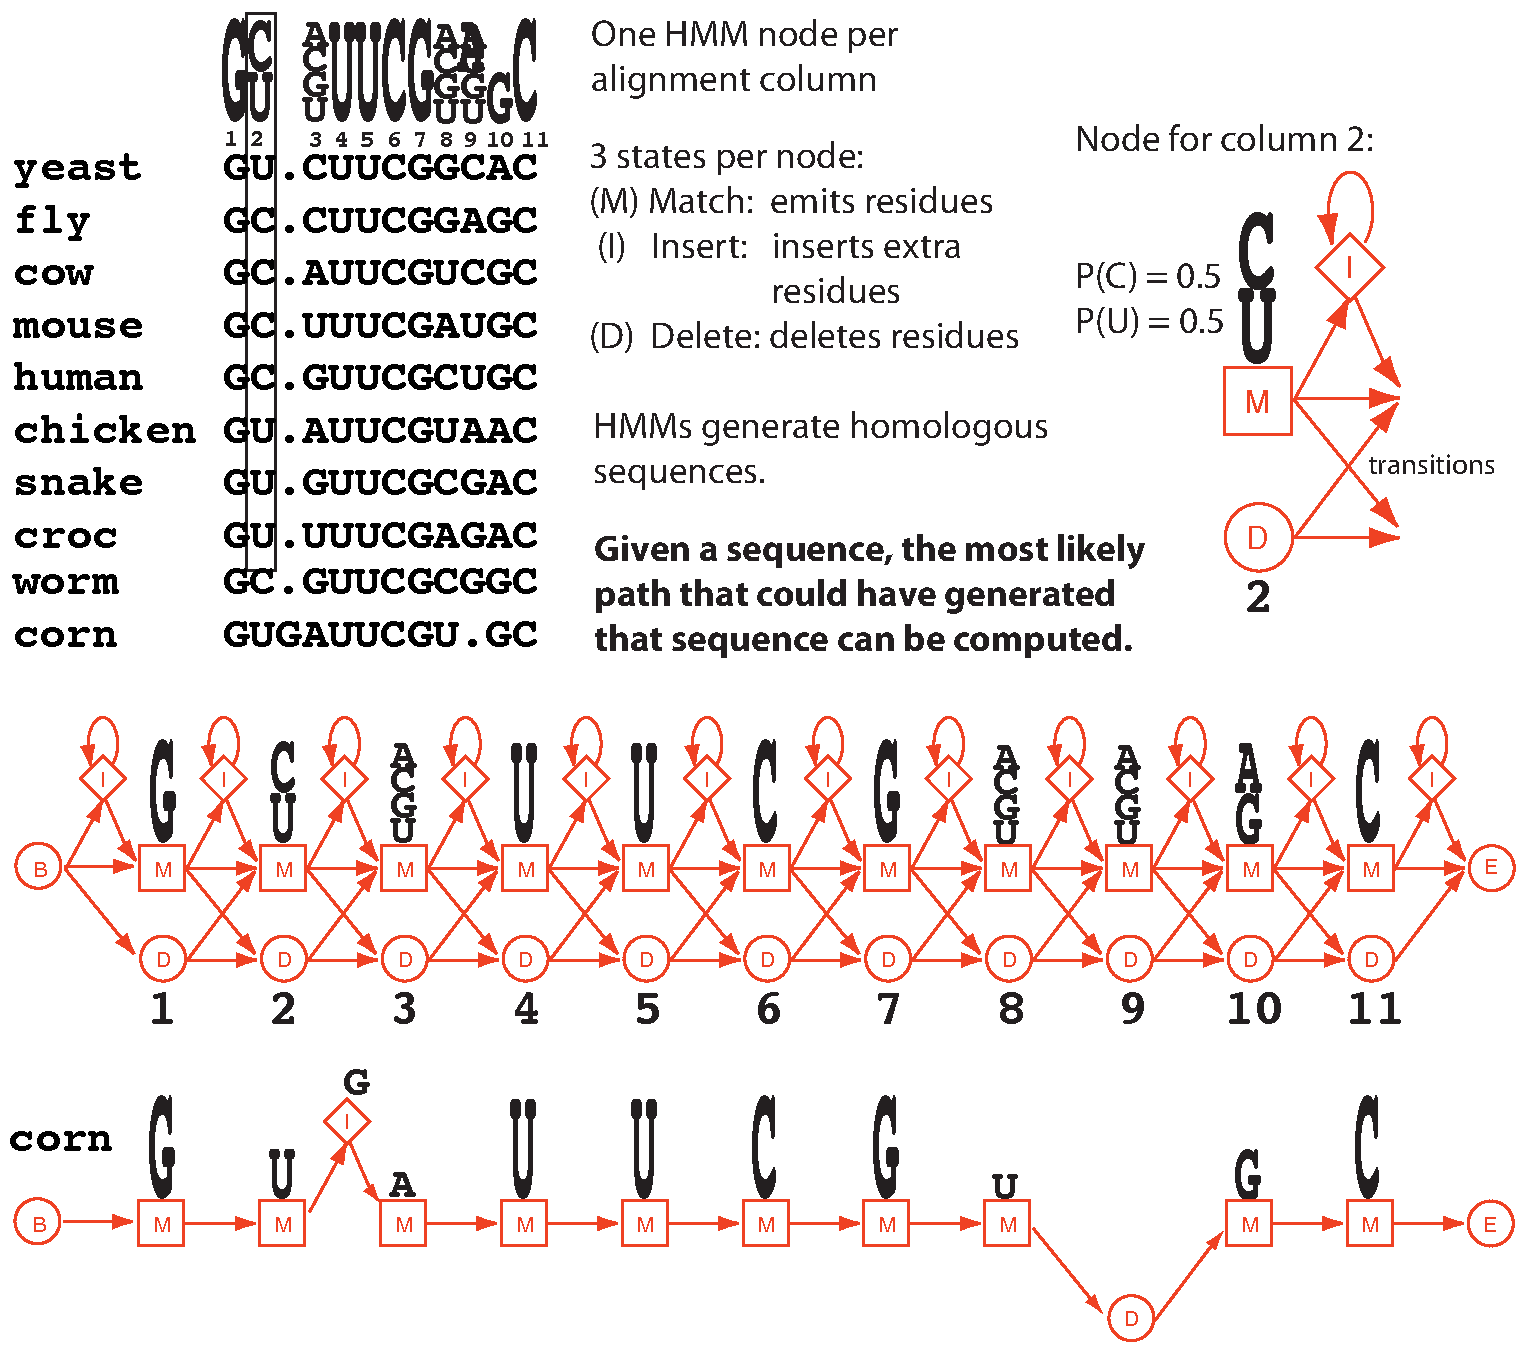
\includegraphics[height=6.625in]{figs/hmm-corn}}
\end{slide}
%%%%%%%%%%%%%%%%%%%%%%%%%%%%%%%%%%%%%%%%%%%%%%%%%%%%%%%%%%%%%%%
\begin{slide}
\begin{center}
%\textbf{profile HMMs and covariance models}
\textbf{Covariance models (CMs) are built \\ from structure-annotated alignments}
\end{center}

\center{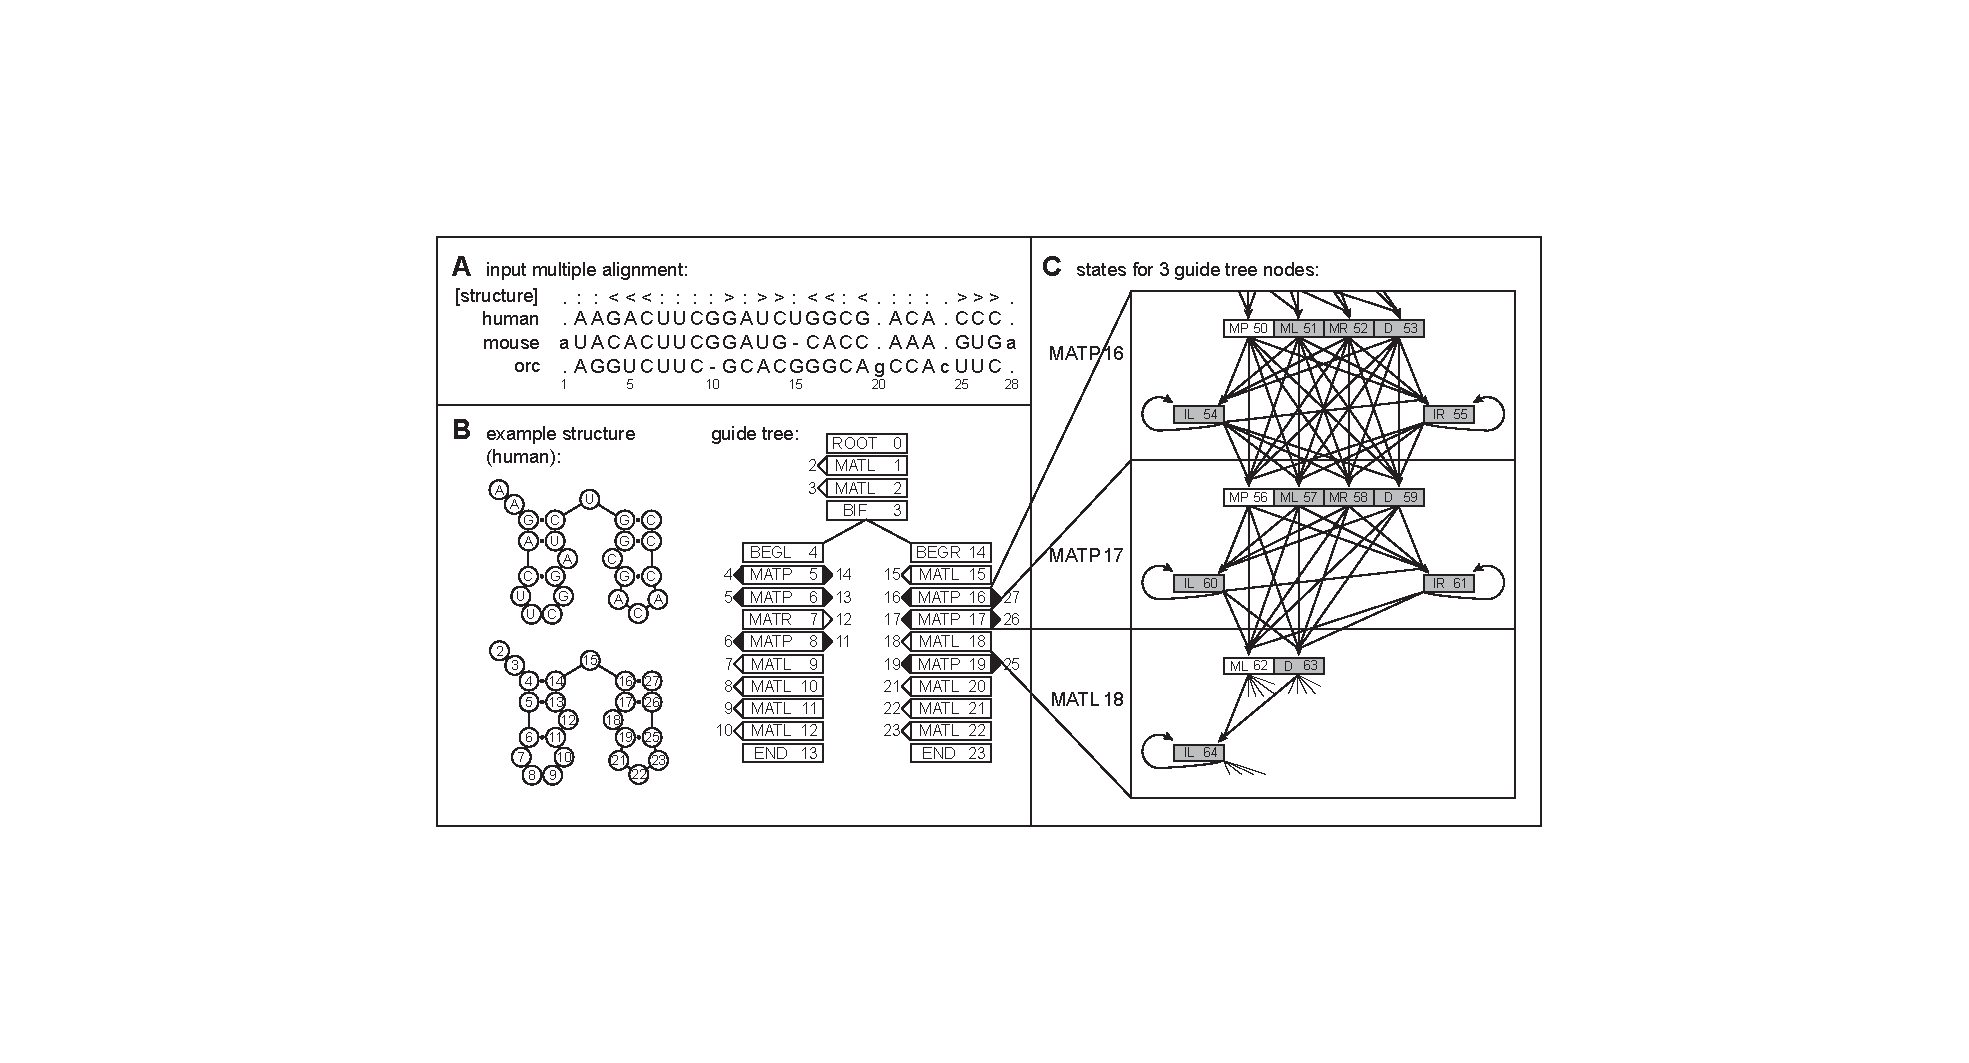
\includegraphics[width=7in]{figs/cmintro_bandcyk}}

\center{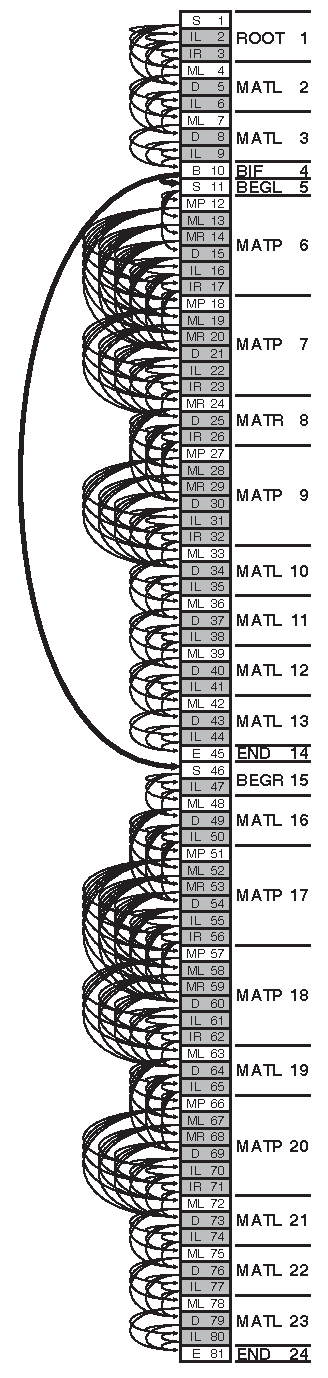
\includegraphics[width=2in,angle=270]{figs/cm-graph-small}}

\vfill

\end{slide}
%%%%%%%%%%%%%%%%%%%%%%%%%%%%%%%%%%%%%%%%%%%%%%%%%%%%%%%%%%%%%%%%%%
\begin{slide}
\begin{center}
\textbf{Is the added complexity worth it? \\
  RMARK: an internal RNA homology search benchmark}
\end{center}
\medskip
\begin{minipage}{7in}
\small
\begin{itemize}
\item
  RMARK construction - for each of the 503 Rfam 7 seed alignments:
  \begin{itemize}
%  \item
%    remove sequences $<$ 70\% average family length
  \item 
    single-linkage cluster sequences by sequence identity \\ given the alignment
  \item 
    look for a \textcolor{blue}{training} cluster and
    \textcolor{red}{testing} cluster such that: 
    \begin{itemize}
    \item
      no \textcolor{blue}{training}/\textcolor{red}{test} sequence pair is $>$ 60\% identical
    \item
      at least five sequences are in the \textcolor{blue}{training} set
    \end{itemize}
  \item
    filter \textcolor{red}{test} set so no two test seqs $>$ 70\% identical 
  \item
    %51 families qualify, with 450 \textcolor{red}{test} sequences
    51 families qualify, with 450 test sequences
  \item
    %\textcolor{red}{test} seqs are embedded in a 1 Mb pseudo-genome (25\% A,C,G,U)
    test seqs are embedded in a 10 Mb pseudo-genome of ``realistic'' base composition
%  \item
%    %    \textsc{BLAST}: family-pairwise search, each \textcolor{blue}{training} seq is used
%        \textsc{BLAST}: family-pairwise search, each \\ training sequence is used
%    as a separate query
%  \item
%    %\textsc{Infernal}: build 1 CM per family from \textcolor{blue}{training} set
%    \textsc{Infernal}: build 1 CM per family from \\ training alignment 
  \end{itemize}
\end{itemize}
\vspace{1.5in}
\end{minipage}
\hspace{0.1in}
\begin{minipage}{3.5in}
  Example: 
\vspace{0.2in}

\begin{center}
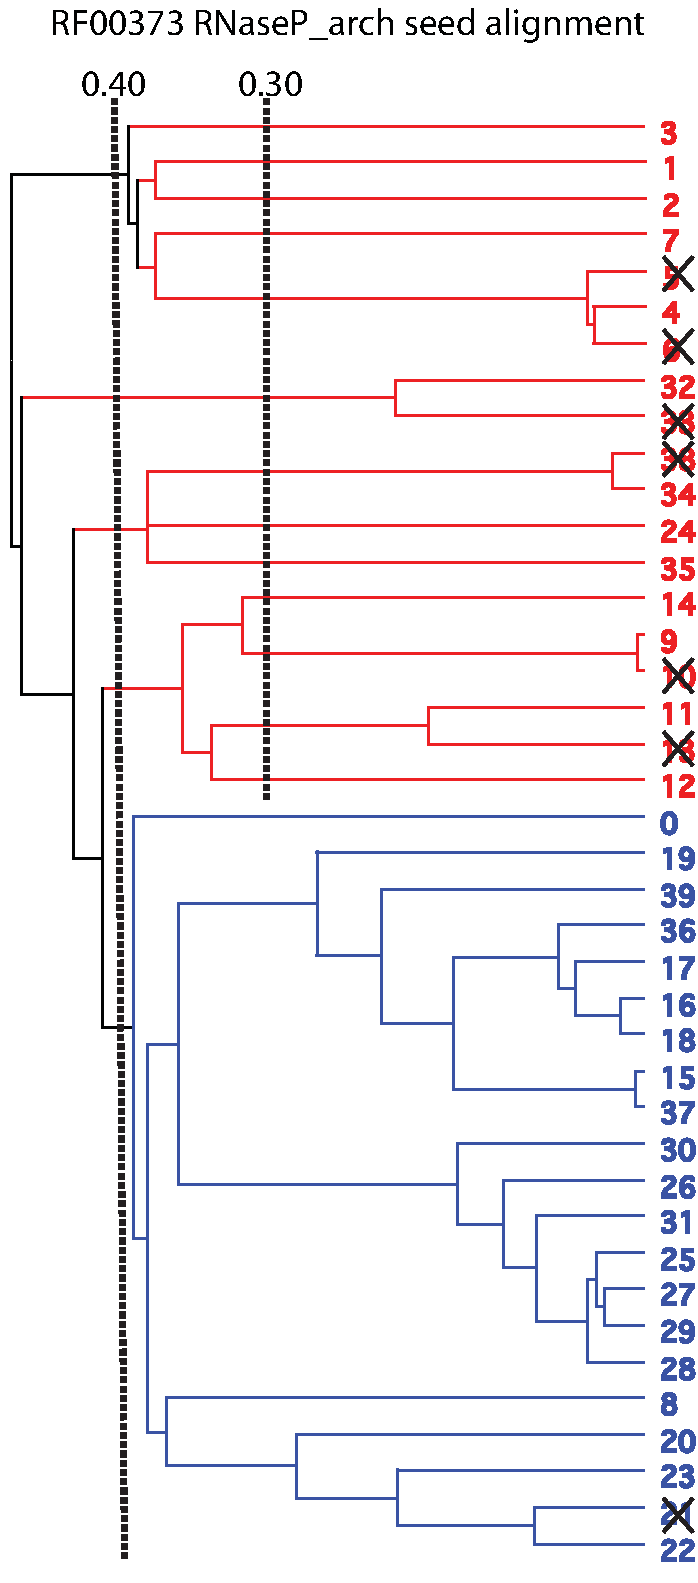
\includegraphics[height=5.5in]{figs/u8-RF00373-tree}

\end{center}
\end{minipage}
\end{slide}
%%%%%%%%%%%%%%%%%%%%%%%%%%%%%%%%%%%%%%%%%%%%%%%%%%%%%%%%%%%%%%%%%%%%%%%%%%
%%%%%%%%%%%%%%%%%%%%%%%%%%%%%%%%%%%%%%%%%%%%%%%%%%%%%%%%%%%%%%%%%%%%%%
\begin{slide}
\begin{center}

\textbf{Infernal outperforms primary-sequence based methods on our
  benchmark (and others\footnote{Freyhult EK, Bollback JP, Gardner
    PP. Genome Res. 2007 17: 117-125.}, not shown)}

\end{center}
\medskip

\center{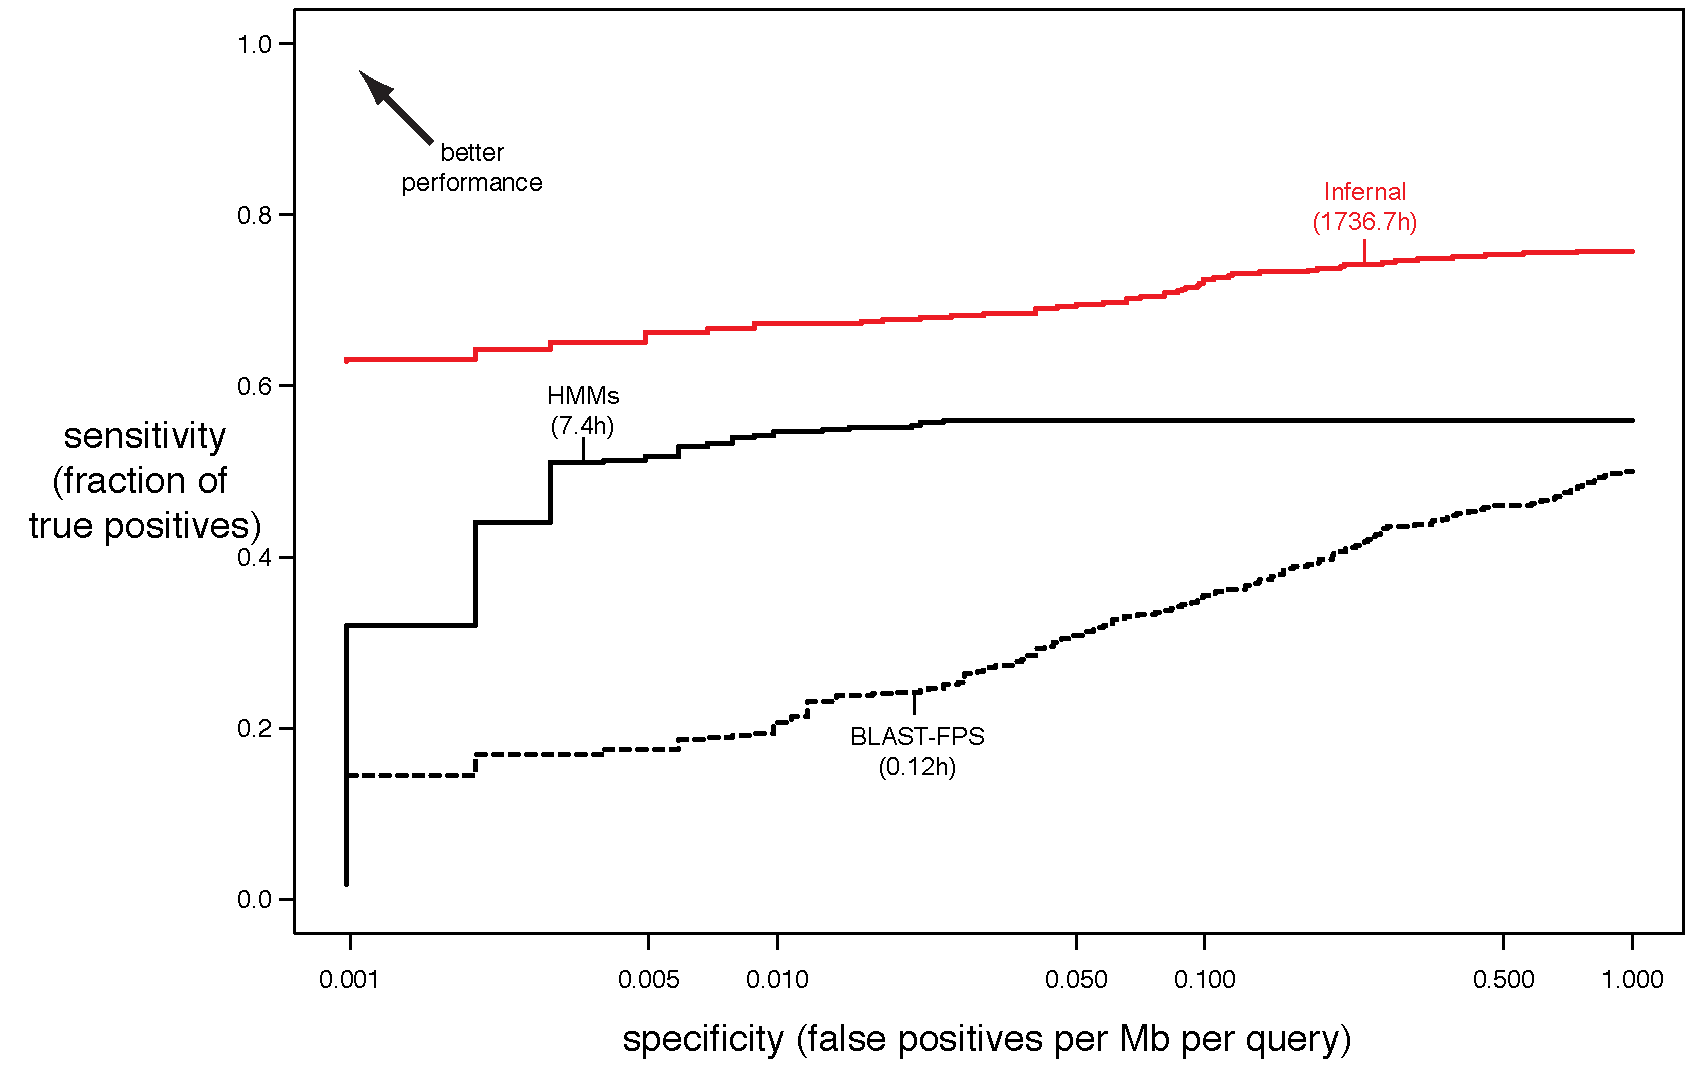
\includegraphics[width=10in]{figs/brown-roc1}}

\vfill 
\end{slide}
%%%%%%%%%%%%%%%%%%%%%%%%%%%%%%%%%%%%%%%%%%%%%%%%%%%%%%%%%%%%%%%%%%%%%%
\begin{comment}
\begin{slide}
\begin{center}
\textbf{Accelerating CM homology search}
\end{center}

\medskip
\small
\begin{itemize}

\item
CM homology search CYK and Inside dynamic programming algorithm \\ scale
$O(LN^2 log N))$ for a database of size $L$ and an RNA of length
$N$

\item Two complementary acceleration heuristic strategies:

\begin{enumerate}
\item 
Decreasing $L$ (prefiltering database) would speed up searches.

\item 
Banded dynamic programming (decreasing $N^2 logN$ part) would speed up searches.

\begin{itemize}
\item 
  HMM banding is lame when there is no primary sequence conservation, \\ which occurs most of the time during searches. 
\item 
  A sequence-independent method would be useful.
\end{itemize}
\end{enumerate}

\end{itemize}

\vfill
\end{slide}
\end{comment}
%%%%%%%%%%%%%%%%%%%%%%%%%%%%%%%%%%%%%%%%%%%%%%%%%%%%%%%%%%%%%%%%%%%%%%%%%%
\begin{slide}
\begin{center}
%\textbf{CMs are much slower than HMMs}
\textbf{CM searches are especially slow for large RNAs}
\medskip

% CM times taken from table 4.2 of my submitted thesis 
% HMM search: viterbi (should be forward), from CPH talk, doubled to 
% match how the table 4.2 times were computed (for both strands of a 1Mb search)
\small
\begin{tabular}{lr|rr|r}
                  &        & \multicolumn{2}{c|}{search (min/Mb)} \\ %\cline{3-4}
                  &        &        & \\
family            & length & HMM    & \textcolor{red}{CM}     & \textcolor{red}{CM/HMM} \\ \hline 
                  &        &        &        & \\
tRNA              & 71     &  0.34  &  \textcolor{red}{27.0}  & \textcolor{red}{79.4}\\
                  &        &        &        & \\
%5S rRNA           & 119    &  0.54  &  \textcolor{red}{26.9}  & \textcolor{red}{49.8}\\
%                  &        &        &        & \\
Lysine riboswitch & 183    &  0.80  & \textcolor{red}{133.2}  & \textcolor{red}{166.7}\\
                  &        &        &        & \\
SRP RNA           & 304    &  1.32  & \textcolor{red}{276.4}  & \textcolor{red}{214.4}\\
                  &        &        &        & \\
RNaseP RNA        & 365    &  1.56  & \textcolor{red}{733.4}  & \textcolor{red}{470.3}\\
                  &        &        &      \\
%SSU rRNA          & 1466   &  0.93 &    - \\
%SSU rRNA          & 1466   &  4.00 & 7660.0&  0.08  & 795.6 \\
%                  &        &        &        &         &  \\
\end{tabular}
\end{center}

\vfill

\end{slide}
%%%%%%%%%%%%%%%%%%%%%%%%%%%%%%%%%%%%%%%%%%%%%%%%%%%%%%%%%%%%%%%%%%%%
%%%%%%%%%%%%%%%%%%%%%%%%%%%%%%%%%%%%%%%%%%%%%%%%%%%%%%%%%%%%%%%%%%%%
\begin{slide}
\begin{center}
\textbf{Why CM homology search is so slow}
\end{center}

\medskip
\small
\begin{itemize}

\item
CM algorithms align/score all subsequences of length
$1..W$ to each state of the model
%looking for high scoring hits
%$1..W$ \\ as they scan along the target sequence
%looking for high scoring hits
\end{itemize}

%\center{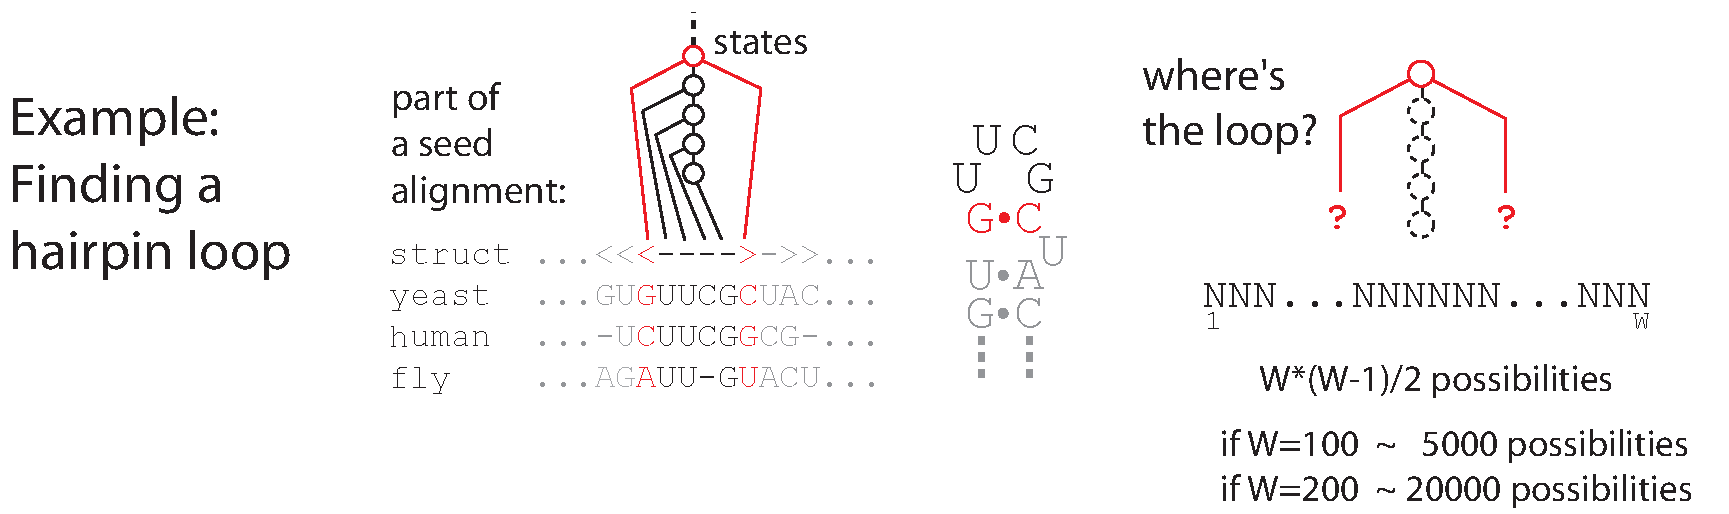
\includegraphics[width=10.4in]{figs/wheresloop}}
\center{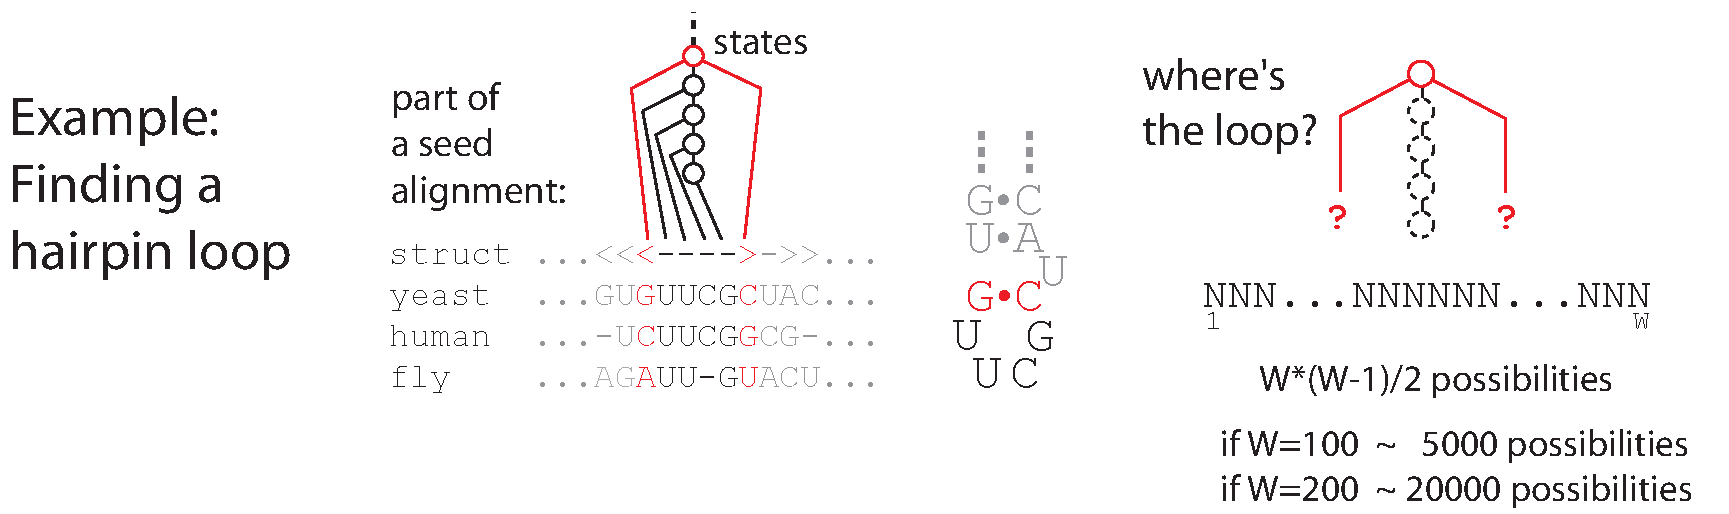
\includegraphics[width=10.4in]{figs/wheresloop-2014}}

  We could save time by restricting the possible loop lengths
  considered.

  {\bf One idea: take advantage of the generative capacity of CMs \\ to generate
  sequences and examine loop length distribution.}

\vfill
\end{slide}
%%%%%%%%%%%%%%%%%%%%%%%%%%%%%%%%%%%%%%%%%%%%%%%%%%%%%%
\begin{comment}
\begin{slide}
\begin{center}
\textbf{CM searches are slow (especially for large RNAs)}
\end{center}

\small
%For a:
%
%\begin{tabular}{l}
%Model of $M$ positions, \\
%a maximum hit length of $W$ nucleotides, \\
%and a database of length $L$: \\
%\end{tabular}

\begin{center}
\begin{tabular}{rllll}
      & \multicolumn{2}{c}{DP algorithms} &          & \\ \cline{2-3}
      & most likely    & sum over       &            &           \\
model & alignment (ML) & all alignments & complexity & DP matrix \\ \hline
& & & & \\
profile HMM & Viterbi & Forward & $O(LN)$        & 2 dimensions \\
& & & & \\
CM          & CYK     &  Inside & $O(LN^2logN)$  & 3 dimensions \\
& & & & \\
%& & & \\
%& & & \\
%\multicolumn{4}{l}{$L$: database length} \\
%\multicolumn{4}{l}{$M$: model length} \\
%\multicolumn{4}{l}{$W$: maximum hit length} \\
%& & & \\
%& & & \\
%& & & \\
%\multicolumn{4}{l}{CYK and Inside fill in a 3-dimensional matrix with
%  $(v,i,j)$ tuples:} \\
\end{tabular}

\medskip

%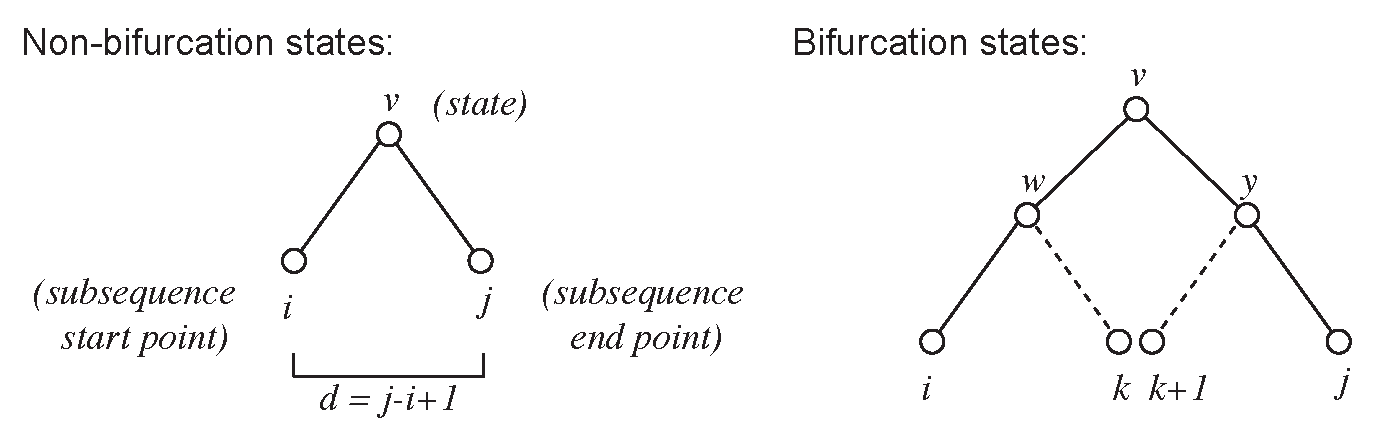
\includegraphics[width=10in]{figs/cm-hmm-complexity}
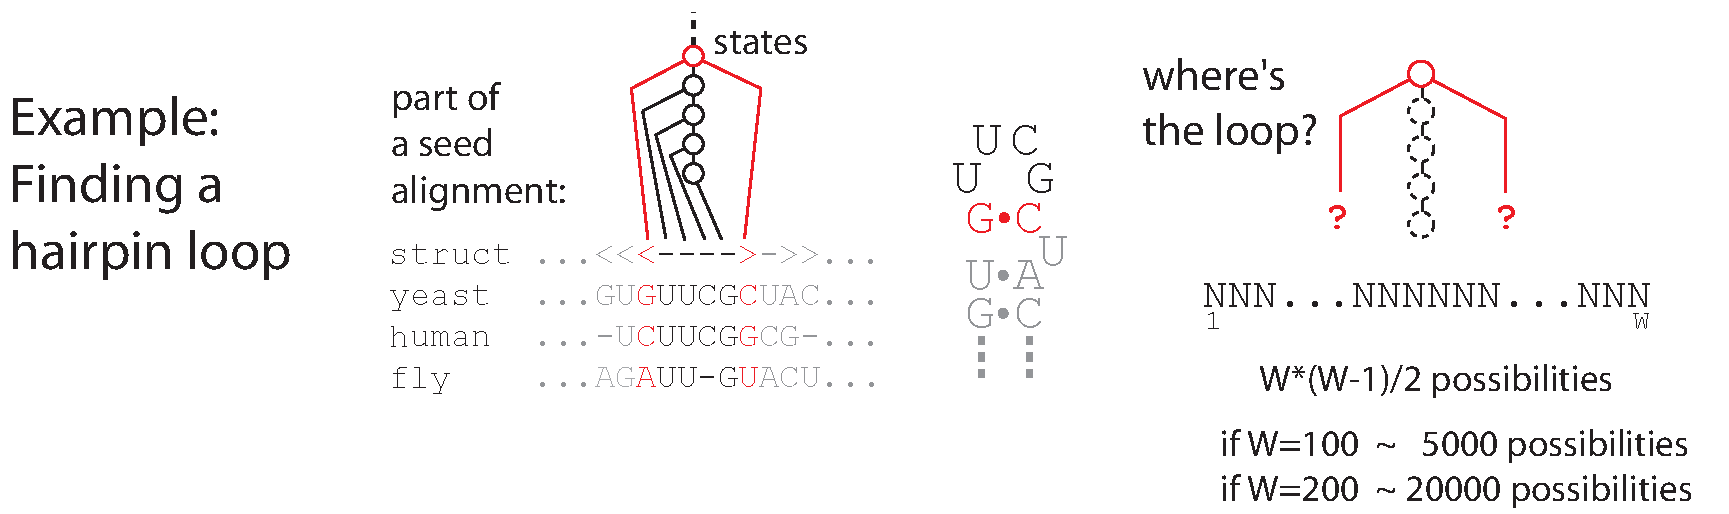
\includegraphics[width=10in]{figs/wheresloop}

\end{center}
\vfill
\end{slide}
\end{comment}
%%%%%%%%%%%%%%%%%%%%%%%%%%%%%%%%%%%%%%%%%%%%%%%%%%%%%%%%%%%%%%%%%%%%%%%%%%
%%%%%%%%%%%%%%%%%%%%%%%%%%%%%%%%%%%%%%%%%%%%%%%%%%%%%%%%%%%%%%%%%%%%%%%%%%%%%%%%%%%%%%%%%%
%COMMENTED OUT - KEPT HERE FOR REFERENCE - THIS IS THE QDB ALGORITHM *WITHOUT* TEXT COLOR%
% Slide X: QDB intro
%
\begin{comment}
\begin{slide}
\begin{center}
\textbf{Query-dependent banding (QDB) strategy}
\end{center}

\tiny
\begin{itemize}
\item
Calculate $\gamma_v(d)$ probability each state $v$ will emit/align to
subsequences of length $d$, for $d = 0..W$

\begin{tabular}{l|l|l}
\multicolumn{3}{l}{for states $v = M-1$ down to $0$:} \\
$v = $ end state $(E)$: & $\gamma_v(0) = 1$ & \\
                        & $\gamma_v(d) = 0$ & for $d=1$ to $W$ \\
& & \\
$v = $ bifurcation $(B)$: & $\gamma_v(d) = \sum_{n=0}^{d} \gamma_y(n)
* \gamma_z(d-n)$ & for $d = 0$ to $W$ \\
& & \\
else ($v = S, P, L, R$): & $\gamma_v(d) = 0$ & for $d=0$ to $(\Delta_v^{L} + \Delta_v^{R} -
1)$ \\
& $\gamma_v(d) = \sum_{y \in C_v} \gamma_y(d-(\Delta_v^{L} + \Delta_v^{R})) * t_v(y) $ 
& for $d = (\Delta_v^{L} + \Delta_v^{R})$ to $W$ \\
\end{tabular}
\flushleft{$\Delta_v^{L}$: number of nucleotides emitted to the left}
\flushleft{$\Delta_v^{R}$: number of nucleotides emitted to the right}

\end{itemize}

\vfill
\end{slide}
\end{comment}
%COMMENTED OUT - KEPT HERE FOR REFERENCE - THIS IS THE QDB ALGORITHM *WITHOUT* TEXT COLOR%
%%%%%%%%%%%%%%%%%%%%%%%%%%%%%%%%%%%%%%%%%%%%%%%%%%%%%%%%%%%%%%%%%%%%%%%%%%%%%%%%%%%%%%%%%%
% Slide X: QDB intro
%
\begin{slide}
\begin{center}
\textbf{Query-dependent banding (QDB) strategy}
\end{center}

\tiny
\begin{itemize}
\item
Calculate \textcolor{red}{$\gamma_v(d)$} probability each state $v$ will emit/align to
subsequences of length $d$, for $d = 0..W$

\begin{tabular}{l|l|l}
\multicolumn{3}{l}{for states $v = M-1$ down to $0$:} \\
$v = $ end state $(E)$: & \textcolor{red}{$\gamma_v(0)$} $= 1$ & \\
                        & \textcolor{red}{$\gamma_v(d)$} $= 0$ & for $d=1$ to $W$ \\
& & \\
$v = $ bifurcation $(B)$: & \textcolor{red}{$\gamma_v(d)$} $= \sum_{n=0}^{d}$ \textcolor{red}{$\gamma_y(n)$}
$*$ \textcolor{red}{$\gamma_z(d-n)$} & for $d = 0$ to $W$ \\
& & \\
else ($v = S, P, L, R$): & \textcolor{red}{$\gamma_v(d)$} $= 0$ & for $d=0$ to $(\Delta_v^{L} + \Delta_v^{R} -
1)$ \\
& \textcolor{red}{$\gamma_v(d)$} $= \sum_{y \in C_v}$ \textcolor{red}{$\gamma_y(d-(\Delta_v^{L} + \Delta_v^{R}))$} * \textcolor{cyan}{$t_v(y)$}
& for $d = (\Delta_v^{L} + \Delta_v^{R})$ to $W$ \\
\end{tabular}
\flushleft{$\Delta_v^{L}$: number of nucleotides emitted to the left}
\flushleft{$\Delta_v^{R}$: number of nucleotides emitted to the right}

\end{itemize}

\vfill
\end{slide}
%%%%%%%%%%%%%%%%%%%%%%%%%%%%%%%%%%%%%%%%%%%%%%%%%%%%%%%%%%%%%%%%%%%%%%%%%%%%%%%%%%%%
%%%%%%%%%%%%%%%%%%%%%%%%%%%%%%%%%%%%%%%%%%%%%%%%%%%%%%%%%%%%%%%%%%%%%%%%%%
% Slide X: QDB intro
%
\begin{slide}
\begin{center}
\textbf{Query-dependent banding (QDB) strategy}
\end{center}

\tiny
\begin{itemize}
\item
Calculate \textcolor{red}{$\gamma_v(d)$} probability each state $v$ will emit/align to
subsequences of length $d$, for $d = 0..W$

\begin{tabular}{l|l|l}
\multicolumn{3}{l}{for states $v = M-1$ down to $0$:} \\
$v = $ end state $(E)$: & \textcolor{red}{$\gamma_v(0)$} $= 1$ & \\
                        & \textcolor{red}{$\gamma_v(d)$} $= 0$ & for $d=1$ to $W$ \\
& & \\
$v = $ bifurcation $(B)$: & \textcolor{red}{$\gamma_v(d)$} $= \sum_{n=0}^{d}$ \textcolor{red}{$\gamma_y(n)$}
$*$ \textcolor{red}{$\gamma_z(d-n)$} & for $d = 0$ to $W$ \\
& & \\
else ($v = S, P, L, R$): & \textcolor{red}{$\gamma_v(d)$} $= 0$ & for $d=0$ to $(\Delta_v^{L} + \Delta_v^{R} -
1)$ \\
& \textcolor{red}{$\gamma_v(d)$} $= \sum_{y \in C_v}$ \textcolor{red}{$\gamma_y(d-(\Delta_v^{L} + \Delta_v^{R}))$} * \textcolor{cyan}{$t_v(y)$}
& for $d = (\Delta_v^{L} + \Delta_v^{R})$ to $W$ \\
\end{tabular}

\end{itemize}
\center{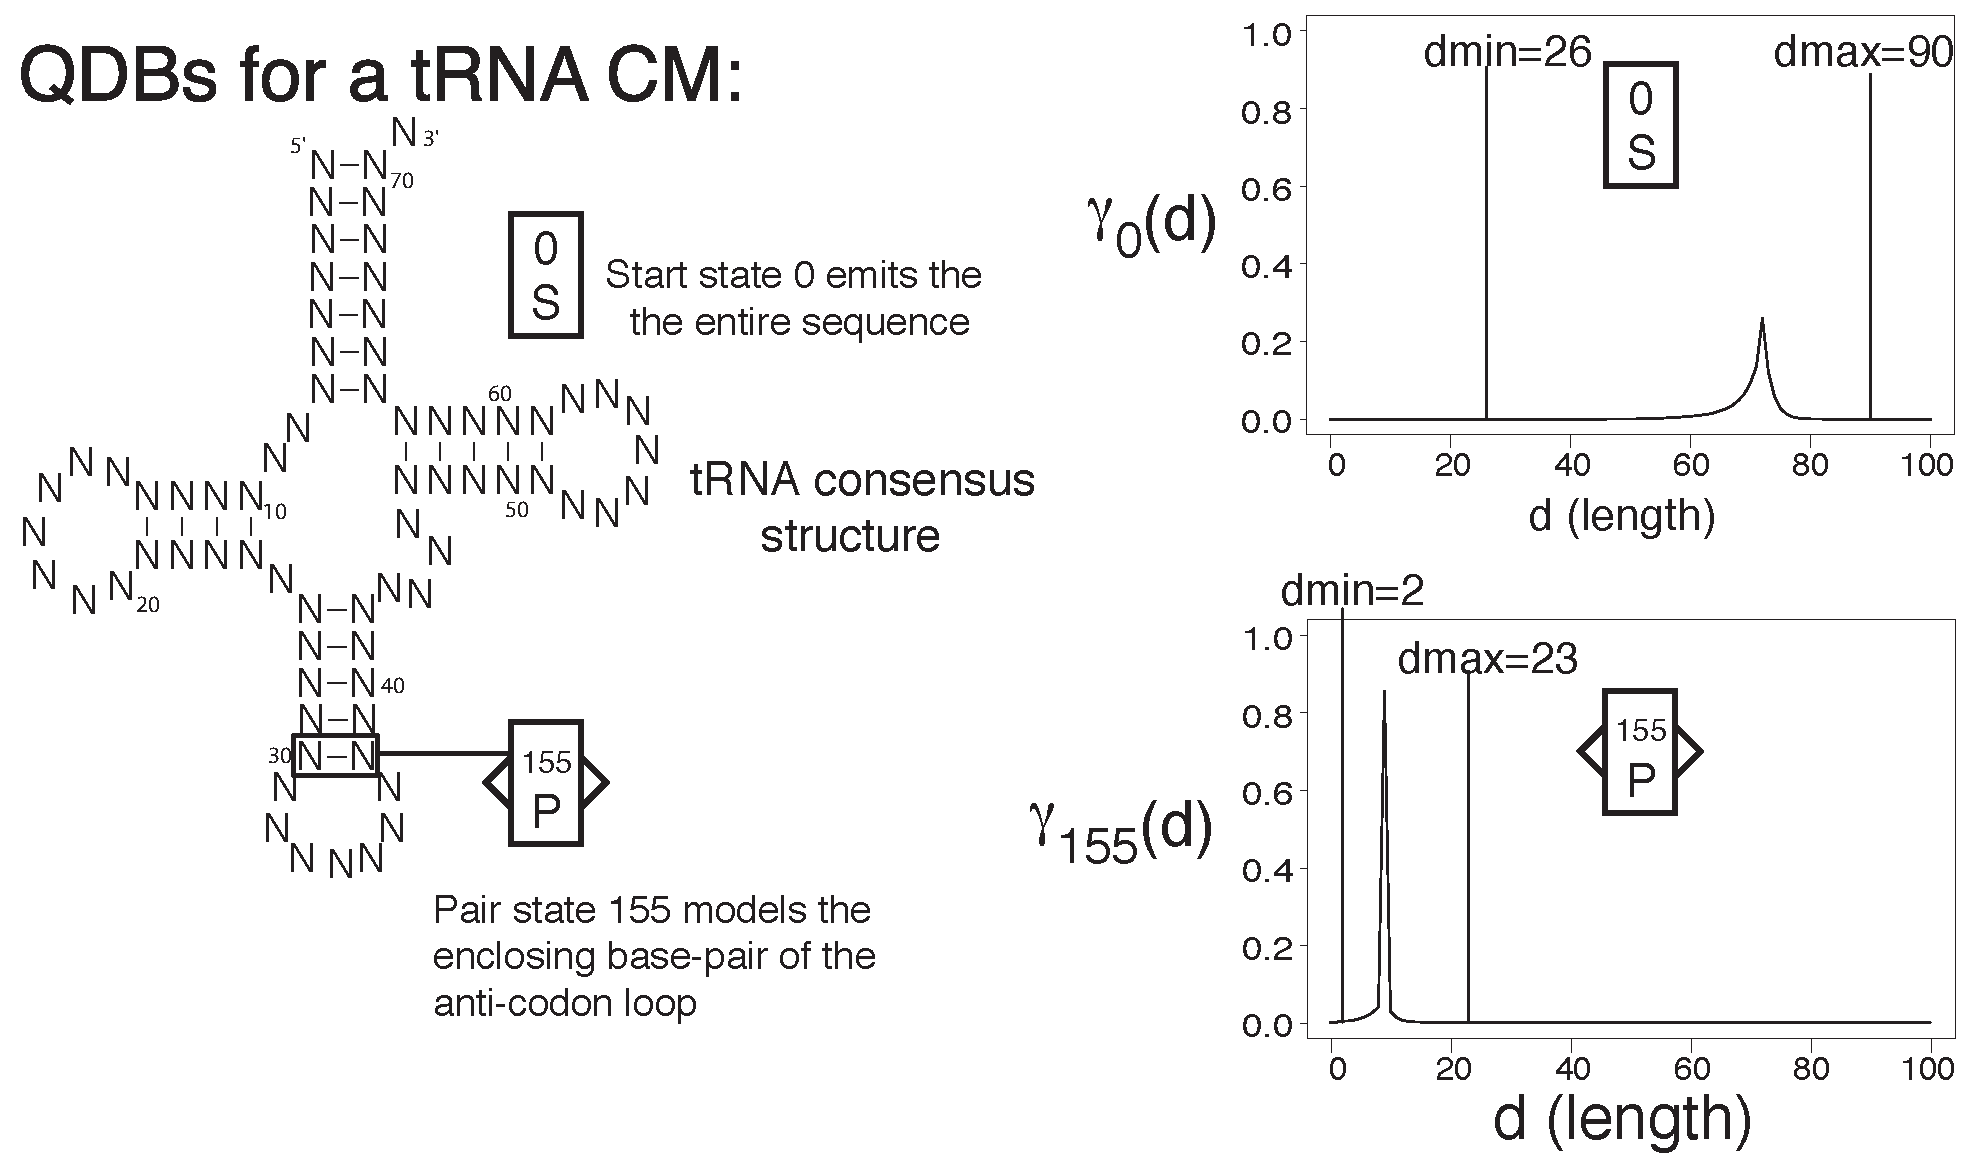
\includegraphics[height=4.5in]{figs/qdb-2014}}

\vfill
\end{slide}
%%%%%%%%%%%%%%%%%%%%%%%%%%%%%%%%%%%%%%%%%%%%%%%%%%%%%%%%%%%%%%%%%%%%%%%%%%%%%%%%%%%%
\begin{slide}
\begin{center}
\textbf{The $\beta$ parameter controls amount of probability loss}
\end{center}

\begin{minipage}{6.5in}

\center{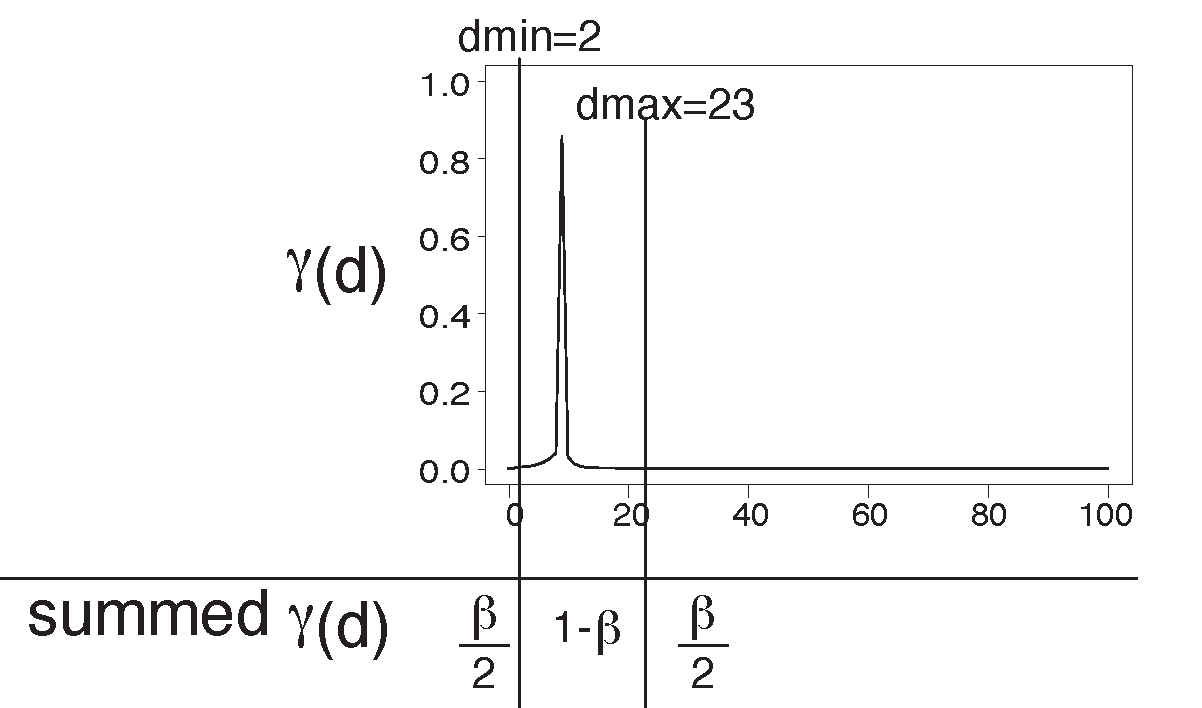
\includegraphics[width=6.5in]{figs/qdb-beta}}

\vspace{1in}
\begin{itemize} 
\small
\item $\beta$ is typically very small: $0.0000001 (10^{-7})$
\medskip
\medskip
\item Higher $\beta$ makes searches faster but less sensitive
\end{itemize}

\vspace{1.5in}
\end{minipage}
\begin{minipage}{4in}

\small

\[
   \sum_{d = 0}^{\mbox{dmin} - 1} \gamma(d) < \frac{\beta}{2}
\]

\[
   \sum_{d = \mbox{dmin}}^{\mbox{dmax}} \gamma(d) = 1 - \beta
\]

\[
   \sum_{d = \mbox{dmax} + 1}^{W} \gamma(d) < \frac{\beta}{2}
\]


\vspace{3in}
\end{minipage}


\end{slide}

%%%%%%%%%%%%%%%%%%%%%%%%%%%%%%%%%%%%%%%%%%%%%%%%%%%%%%
\begin{comment}
\begin{slide}
\begin{center}
\textbf{Choice of probability loss ($\beta$ parameter)}
\end{center}

\small


\center{\includegraphics[width=10in]{figs/betavaried}}

\vfill
\end{slide}
\end{comment}
%%%%%%%%%%%%%%%%%%%%%%%%%%%%%%%%%%%%%%%%%%%%%%%%%%%%%%%%
\begin{slide}
\begin{center}
\textbf{Empirical time complexity of CM homology search}
\end{center}

\center{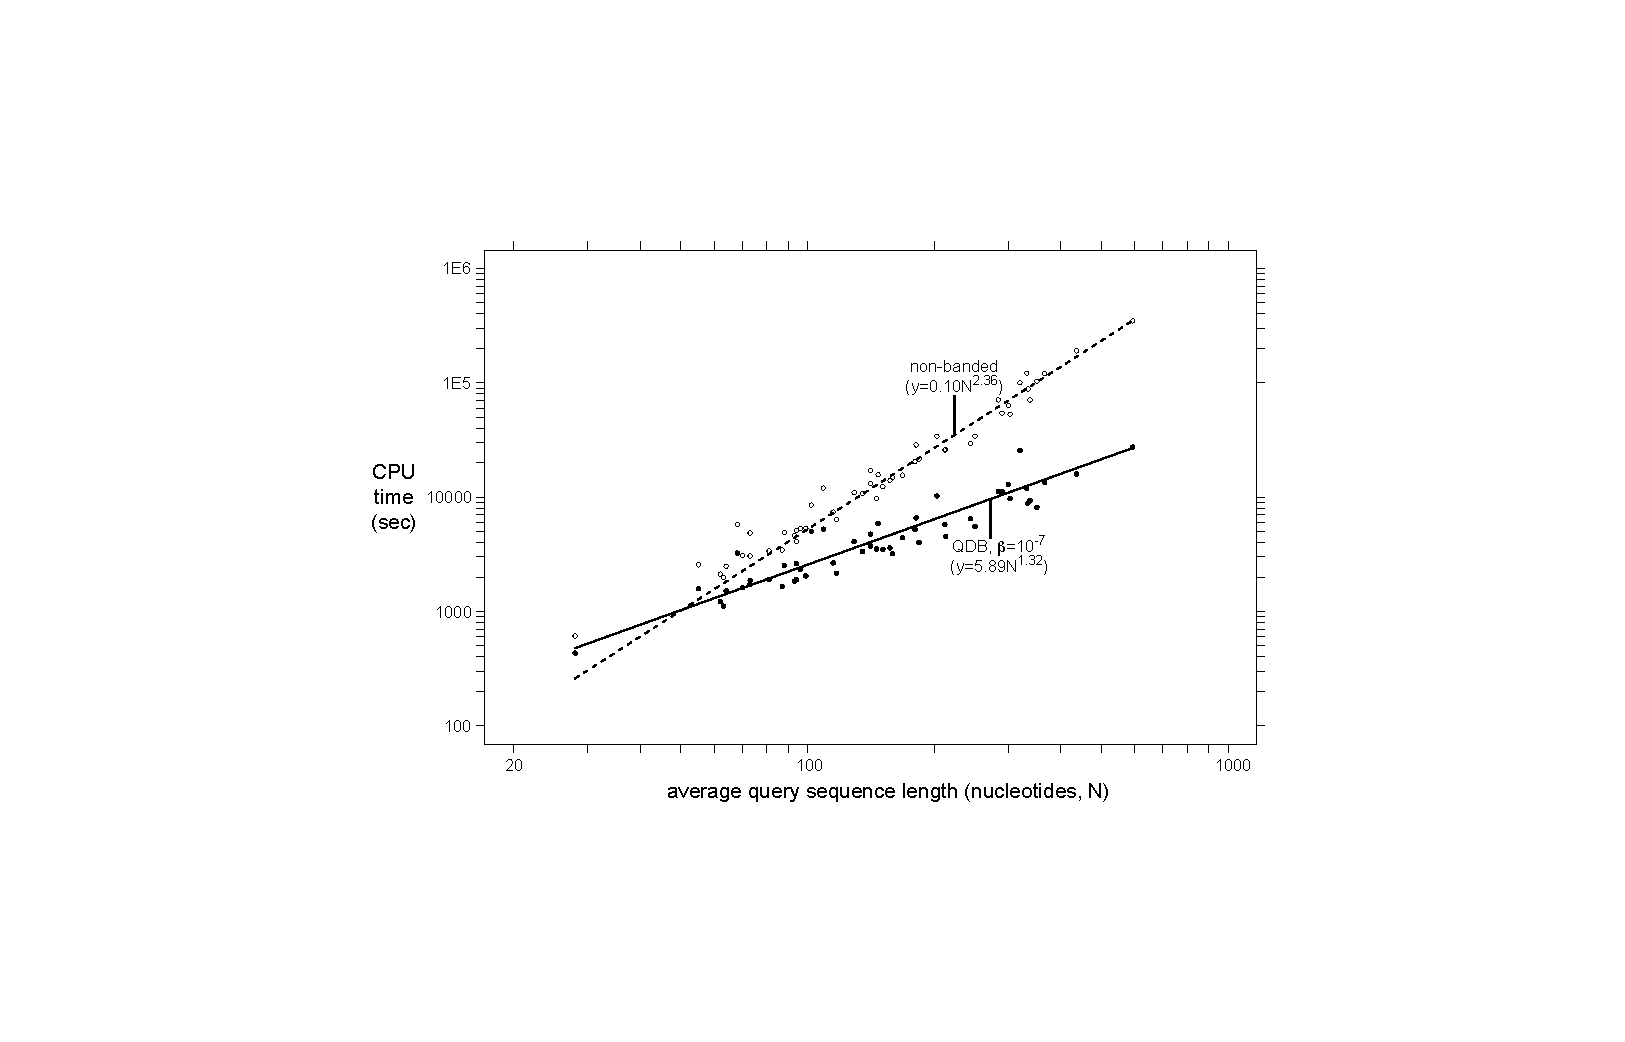
\includegraphics[width=10in]{figs/speedup}}

\vfill
\end{slide}

%%%%%%%%%%%%%%%%%%%%%%%%%%%%%%%%%%%%%%%%%%%%%%%%%%%%%%%%%%%%%%%%%%%%%%%%%%%%%%%%%%%%
\begin{slide}
\begin{center}
\textbf{QDB sacrifices very little sensitivity and gives 6-fold speedup}
\end{center}

\center{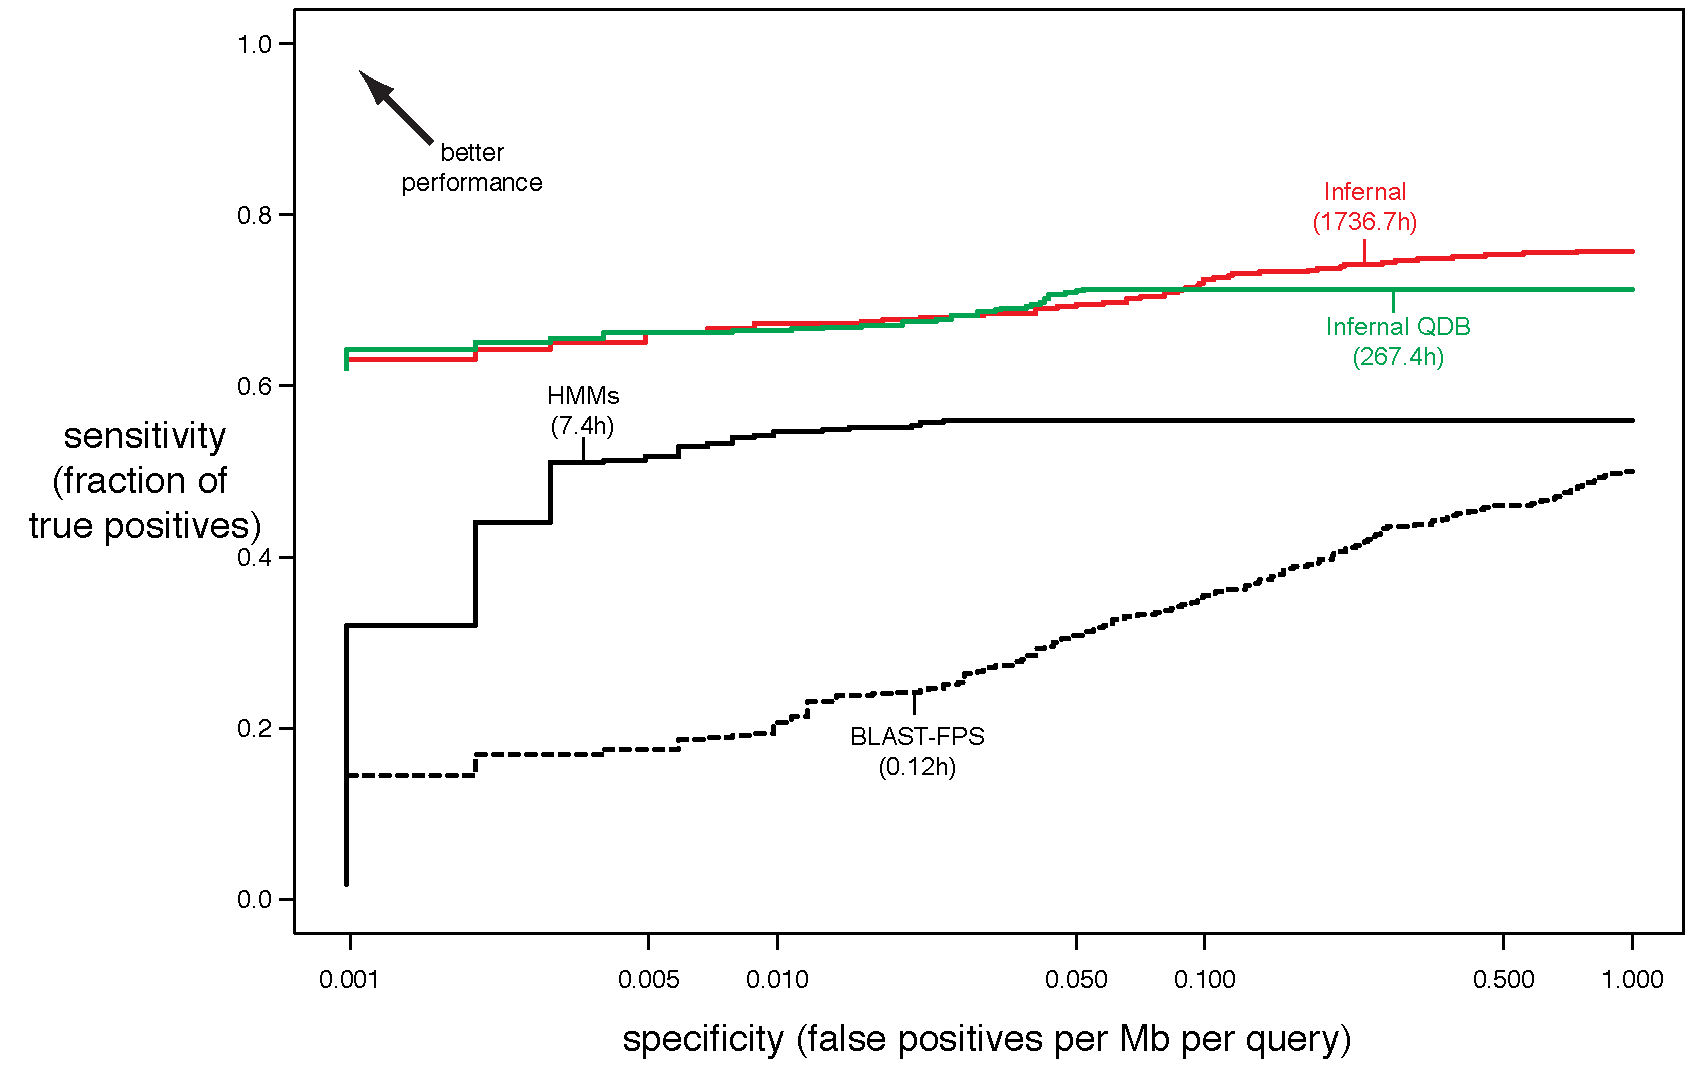
\includegraphics[width=10in]{figs/brown-roc2}}

\vfill
\end{slide}

%%%%%%%%%%%%%%%%%%%%%%%%%%%%%%%%%%%%%%%%%%%%%%%%%%%%%%%%%%%%%%%%%%%%%%%%%%%%%%%%%%%%
\begin{slide}
\begin{center}
\textbf{CM homology searches are still slow}
\end{center}

%timings: QDB, took regular CM times and divided by speedup
%         for QDB paper table 5. For SSU, ran cmsearch 1.0 --forecast
\small
\begin{center}
\small
\begin{tabular}{lr|rr|r|r}
                  &        & \multicolumn{2}{c|}{search (min/Mb)} & \multicolumn{2}{c}{}\\ \cline{3-4}
%                  &        &        &        &            &         \\
                  &        &        &        & \textcolor{mygreen}{QDB}  & non-banded        \\
family            & length & HMM    & \textcolor{mygreen}{QDB CM} & \textcolor{mygreen}{CM/HMM} & CM/HMM  \\ \hline
                  &        &        &        &            &         \\
tRNA              & 71     &  0.34  &  \textcolor{mygreen}{9.6}   & \textcolor{mygreen}{28.2} & \textcolor{black}{79.4}\\
                  &        &        &        &            &         \\
%5S rRNA           & 119    &  0.54  &  \textcolor{mygreen}{9.1}   & \textcolor{mygreen}{16.9} & \textcolor{black}{49.8}\\
%                  &        &        &        &            &         \\
Lysine riboswitch & 183    &  0.80  &  \textcolor{mygreen}{33.8}  & \textcolor{mygreen}{42.3} & \textcolor{black}{166.7}\\
                  &        &        &        &            &         \\
SRP RNA           & 304    &  1.32  &  \textcolor{mygreen}{50.5}  & \textcolor{mygreen}{38.3} & \textcolor{black}{214.4}\\
                  &        &        &        &            &         \\
RNaseP RNA        & 365    &  1.56  &  \textcolor{mygreen}{81.6}  & \textcolor{mygreen}{52.3} & \textcolor{black}{470.3}\\
                  &        &        &        &            &         \\
\end{tabular}
\end{center}

\vfill

\end{slide}
%%%%%%%%%%%%%%%%%%%%%%%%%%%%%%%%%%
\begin{slide}

\begin{center}
\textbf{Filtering as a complementary acceleration strategy}
\end{center}

%\item
%  Query-dependent banding (QDB) accelerates
%  homology search six-fold at a negligible cost to sensitivity
\small
\begin{itemize}
\item
  Main idea: search database with faster method first, hits above some threshold \\ survive the filter and are searched with the slow CM.
%\item
%  Goal of filtering: Maximal speedup with minimal loss of sensitivity
%\item
%  Rfam uses a BLAST filter at an unknown cost to sensitivity
%\item
%  \emph{tRNAscan-SE}: filters database using tRNA-specific heuristics to find tRNAs
\item
  Weinberg and Ruzzo\footnote{Weinberg Z, Ruzzo WL. 22(1):35–39,
    2006.} developed HMM filters for faster searches.
\item
  Others have also worked on this (Sun and Buhler 
  \footnote{Sun Y, Buhler J, Comput. Systems
  Bioinf., p145-156, 2008.}, Zhang and Bafna\footnote{Zhang S et al.,
  Bioinformatics. 22(14):e557-e565, 2006.})
\end{itemize}

\center{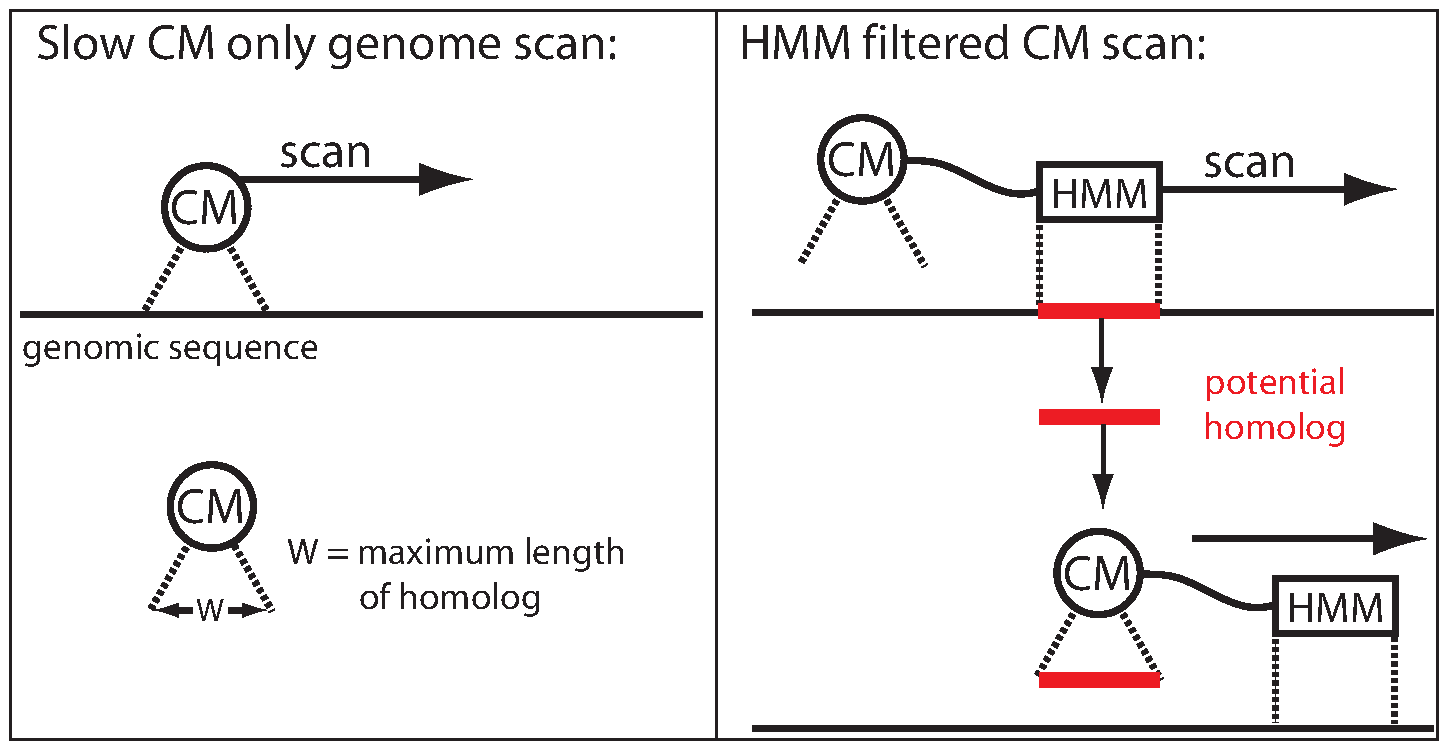
\includegraphics[width=8in]{figs/filter}}
\vfill

\end{slide}
%%%%%%%%%%%%%%%%%%%%%%%%%%%%%%%%%%%%%%%%%%%%%%%%%%%%%%%%%%%%%%%%%%%%%%%%%%
%%%%%%%%%%%%%%%%%%%%%%%%%%%%%%%%%%
\begin{slide}

\begin{center}
\textbf{HMM filters achieve 10-fold speedup at very small cost to accuracy}
\end{center}

\center{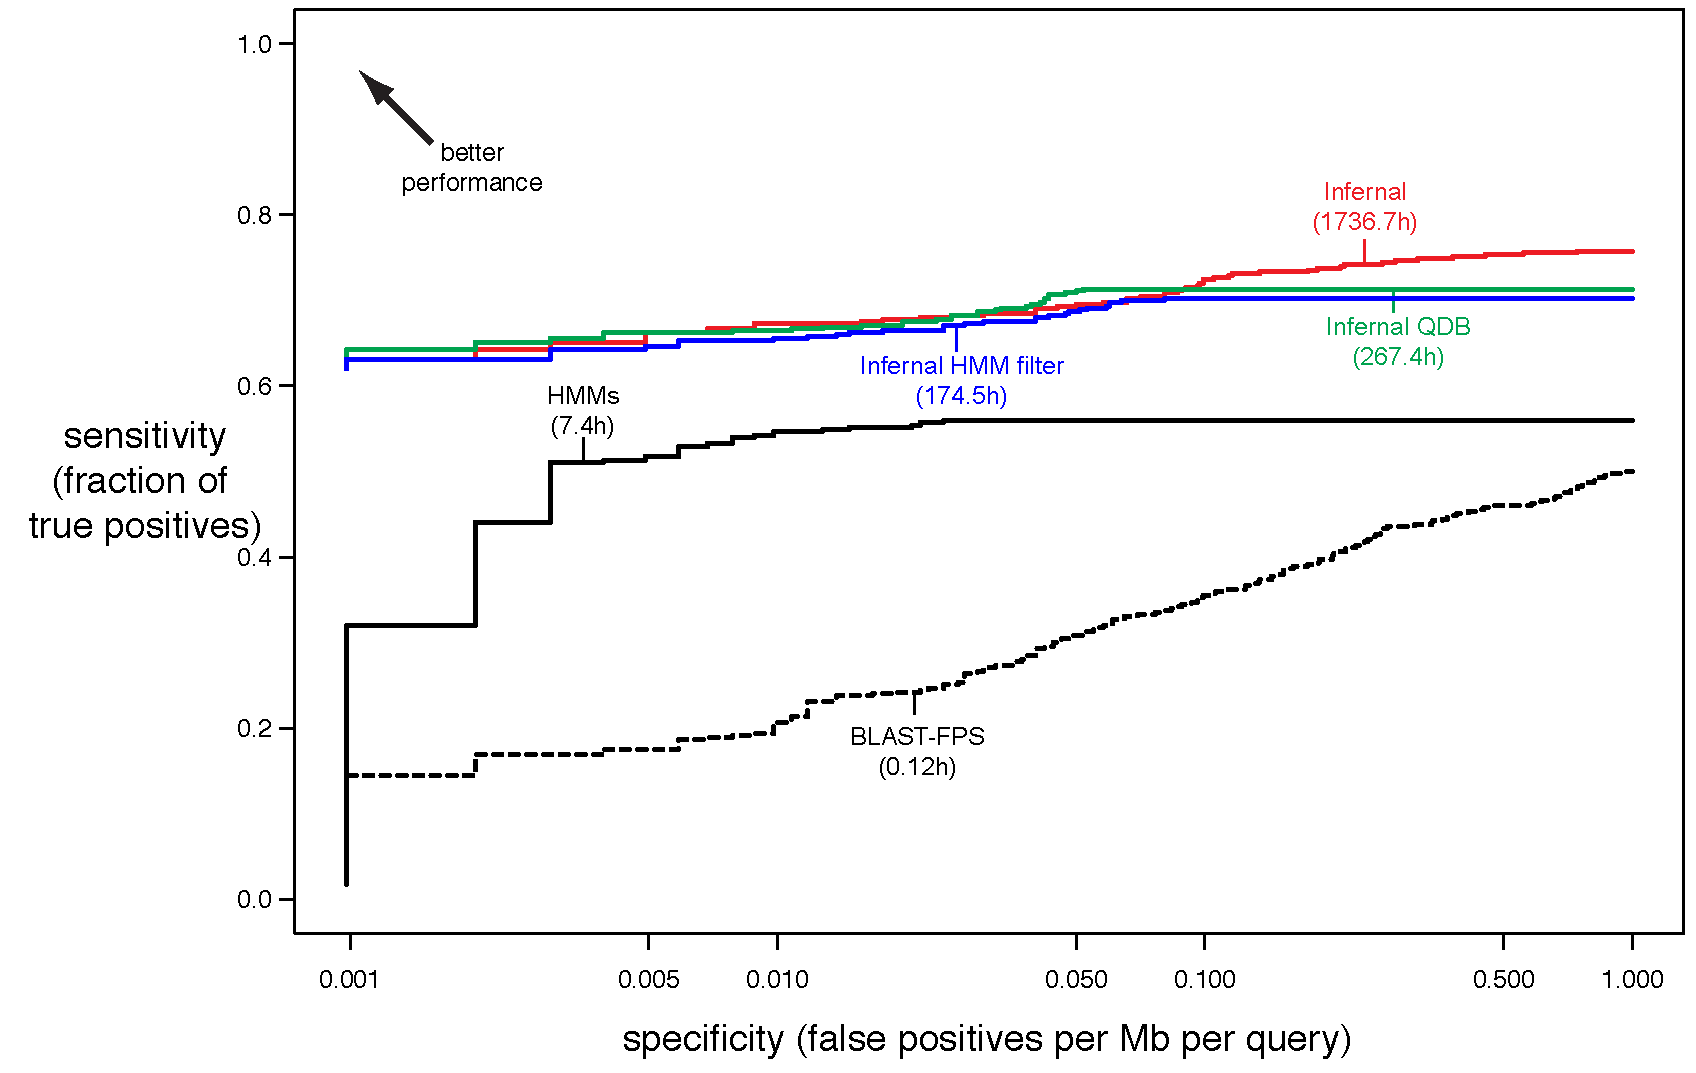
\includegraphics[width=10in]{figs/brown-roc3}}

\vfill

\end{slide}
%%%%%%%%%%%%%%%%%%%%%%%%%%%%%%%%%%
\begin{slide}

\begin{center}
\normalsize
\textbf{Combining QDB and HMM filters yields greater acceleration}

\small
%
The more powerful, slower Inside algorithm is used post-filtering.

Infernal is now 30-fold faster and slightly more sensitive.
%

\end{center}

\center{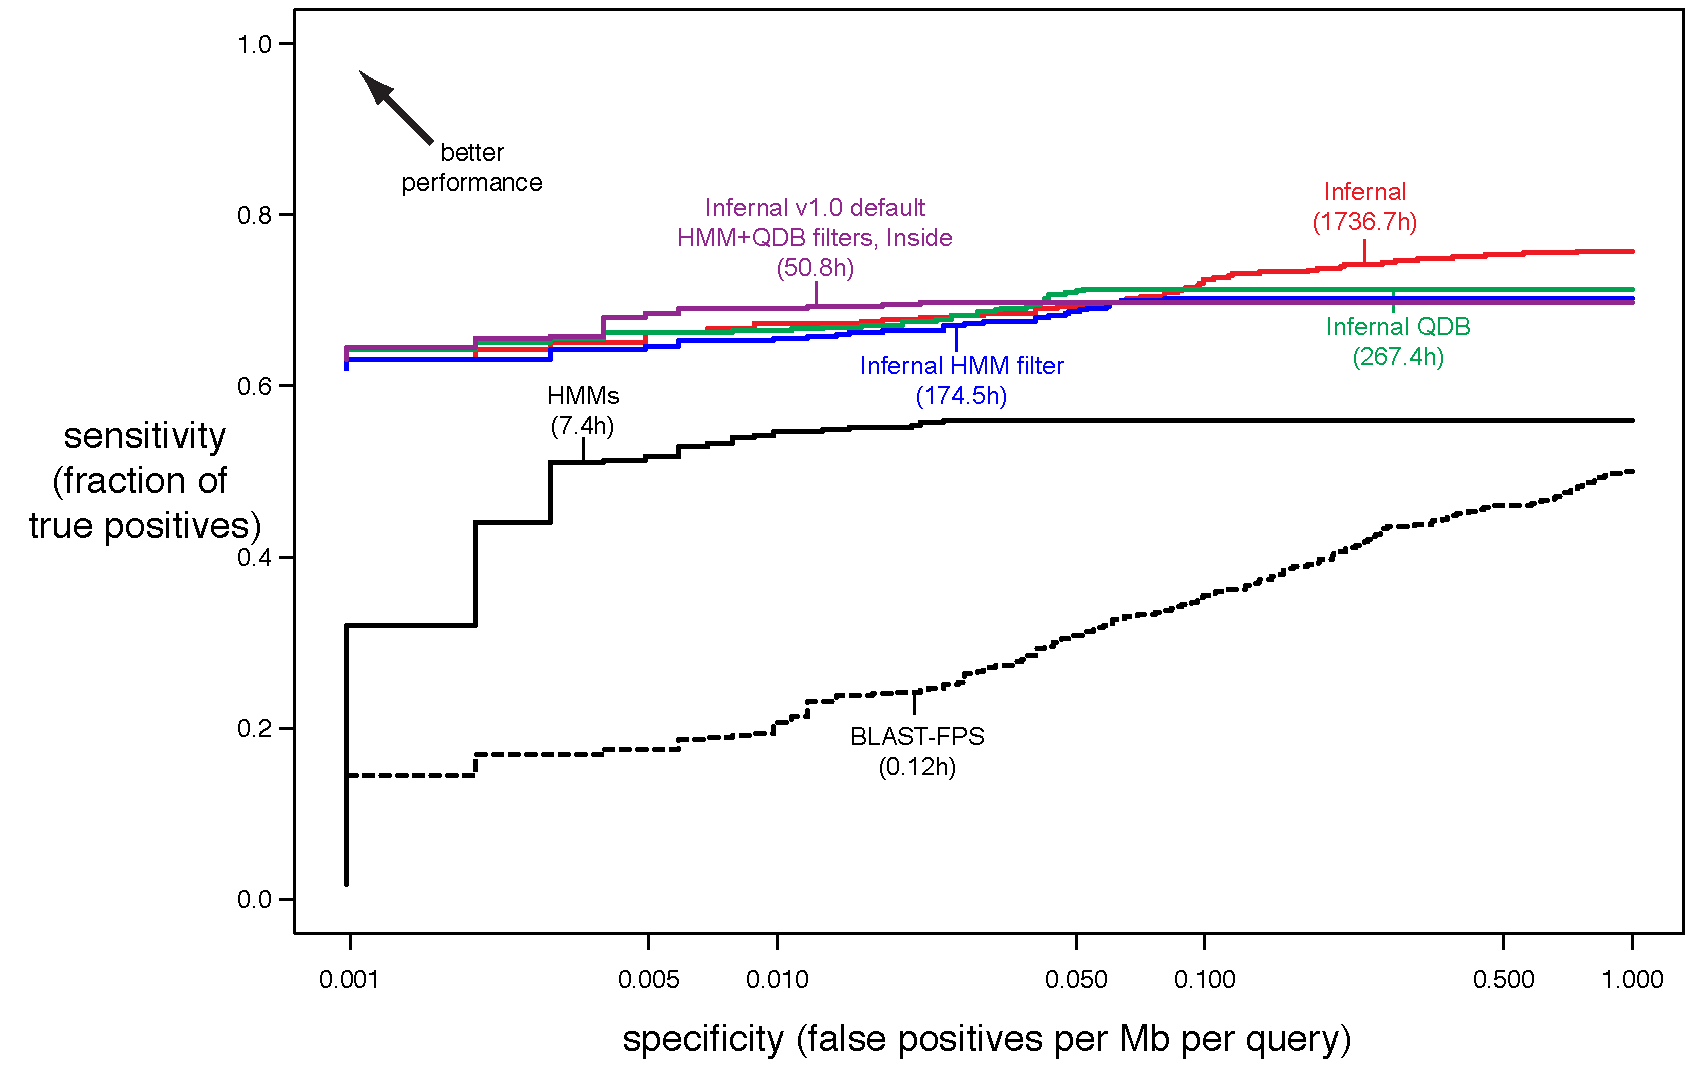
\includegraphics[width=10in]{figs/brown-roc4}}

\vfill

\end{slide}
%%%%%%%%%%%%%%%%%%%%%%%%%%%%%%%%%%
\begin{slide}
\begin{center}

  \textbf{CMs are nearly as fast as HMMs (usually)}
\end{center}


\small
\begin{center}
\small
\begin{tabular}{lr|rr|r|r}
                  &        & \multicolumn{2}{c|}{search (min/Mb)} & \multicolumn{2}{c}{}\\ \cline{3-4}
                  &        &        &        &            &         \\

                  &        &        & \textcolor{mypurple}{HMM+QDB}    & \textcolor{mypurple}{HMM+QDB}  & \\
                  &        &        & \textcolor{mypurple}{filtered}   & \textcolor{mypurple}{filtered}& non-banded        \\
family            & length & HMM    & \textcolor{mypurple}{CM}     & \textcolor{mypurple}{CM/HMM} & CM/HMM  \\ \hline
                  &        &        &        &            &         \\
tRNA              & 71     &  0.34  &  \textcolor{mypurple}{8.8}   & \textcolor{mypurple}{25.9} & \textcolor{black}{79.4}\\
                  &        &        &        &            &         \\
Lysine riboswitch & 183    &  0.80  &  \textcolor{mypurple}{2.2}   & \textcolor{mypurple}{2.8}  & \textcolor{black}{166.7}\\
                  &        &        &        &            &         \\
SRP RNA           & 304    &  1.32  &  \textcolor{mypurple}{6.0}   & \textcolor{mypurple}{4.5} & \textcolor{black}{214.4}\\
                  &        &        &        &            &         \\
RNaseP RNA        & 365    &  1.56  &  \textcolor{mypurple}{1.8}   & \textcolor{mypurple}{1.2} & \textcolor{black}{470.3}\\
                  &        &        &        &            &         \\

\end{tabular}
\end{center}

\vfill

\end{slide}
%%%%%%%%%%%%%%%%%%%%%%%%%%%%%%%%%%%%%%%%%%%%%%%%%%%%%%%%%%%%%%%%%%%%
\begin{slide}
\textcolor{white}{a}
\medskip
\medskip
\medskip
\medskip
\medskip
\center{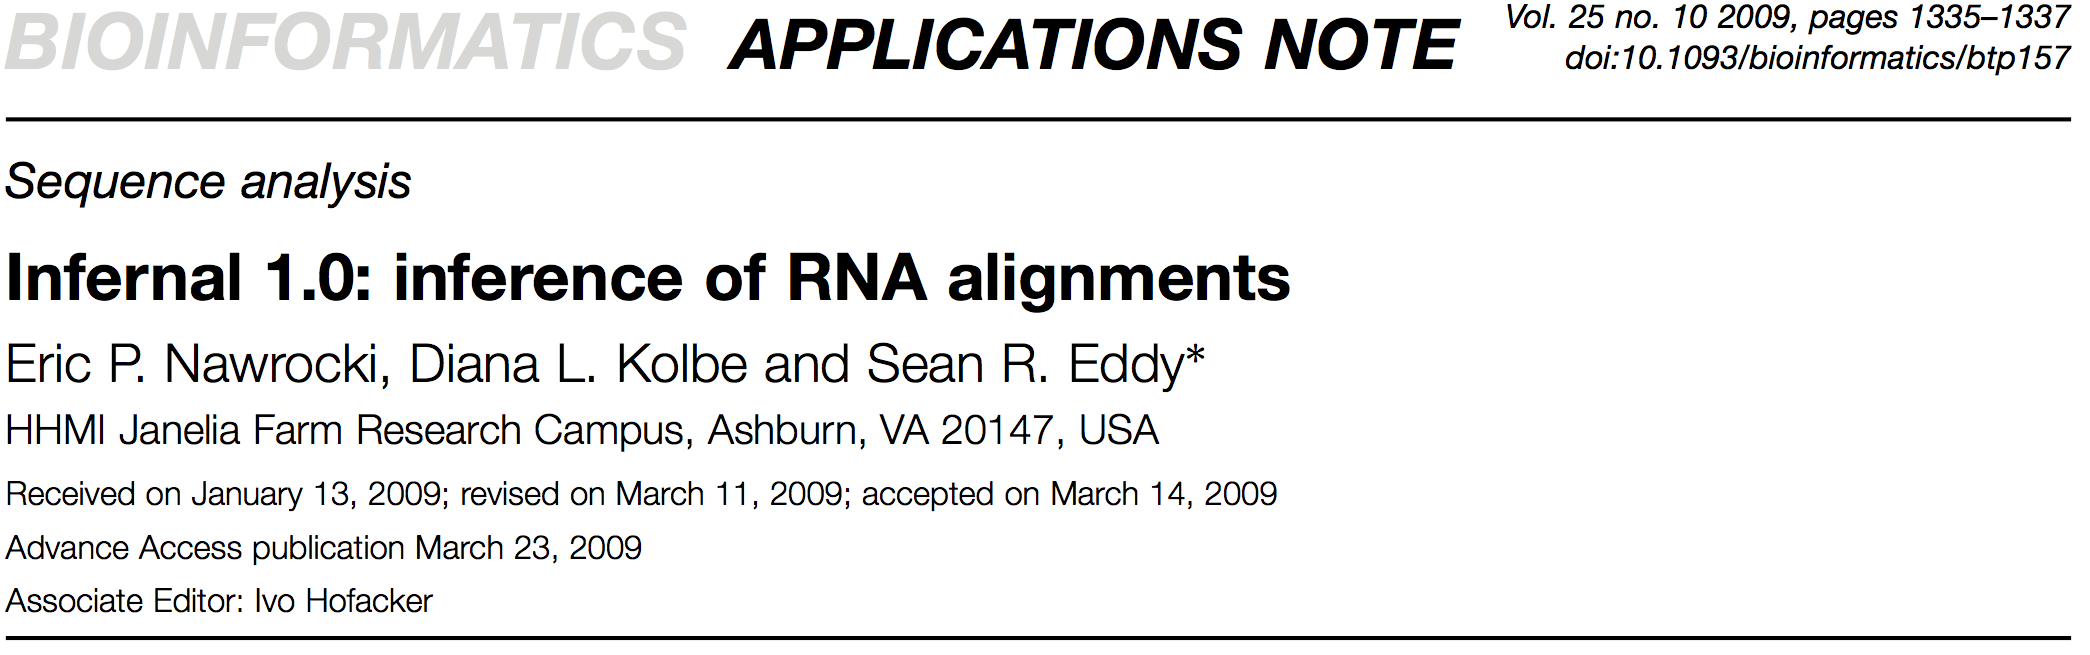
\includegraphics[width=10in]{figs/pub-title-1p0}}
\vfill
\end{slide}
%%%%%%%%%%%%%%%%%%%%%%%%%%%%%%%%%%%%%%%%%%%%%%%%%%%%%%%%%%%%%%%%%%%%%%%%%%
\begin{slide}
\begin{center}
  \textbf{With HMMER3, HMMs got about 100x faster using an MSV filter}
\end{center}

\medskip

\begin{itemize}

\small
\item MSV (Multiple Segment Viterbi) algorithm, which disallows inserts
  and deletes, can be computed using 16-fold vector parallelism with
  low-precision (8-bit) scores\footnote{Eddy SR. PLoS Comp. Biol., 7:e1002195, 2011}.

\end{itemize}

\center{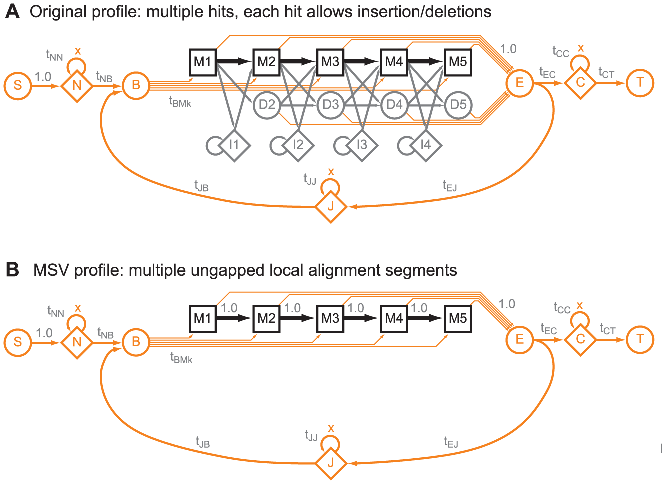
\includegraphics[height=6in]{figs/msv-trunc}}

\vfill 
\end{slide}
%%%%%%%%%%%%%%%%%%%%%%%%%%%%%%%%%%%%%%%%%%%%%%%%%%%%%%%%%%%%%%%%%%%%%%%%%%
\begin{slide}
\begin{center}

  \textbf{The HMM filter step only takes about 15\% \\ of the total Infernal
    running time (7.4h out of 50.8h)}
\end{center}

\medskip
\center{So they won't help unless we further accelerate the downstream CM step.}

\center{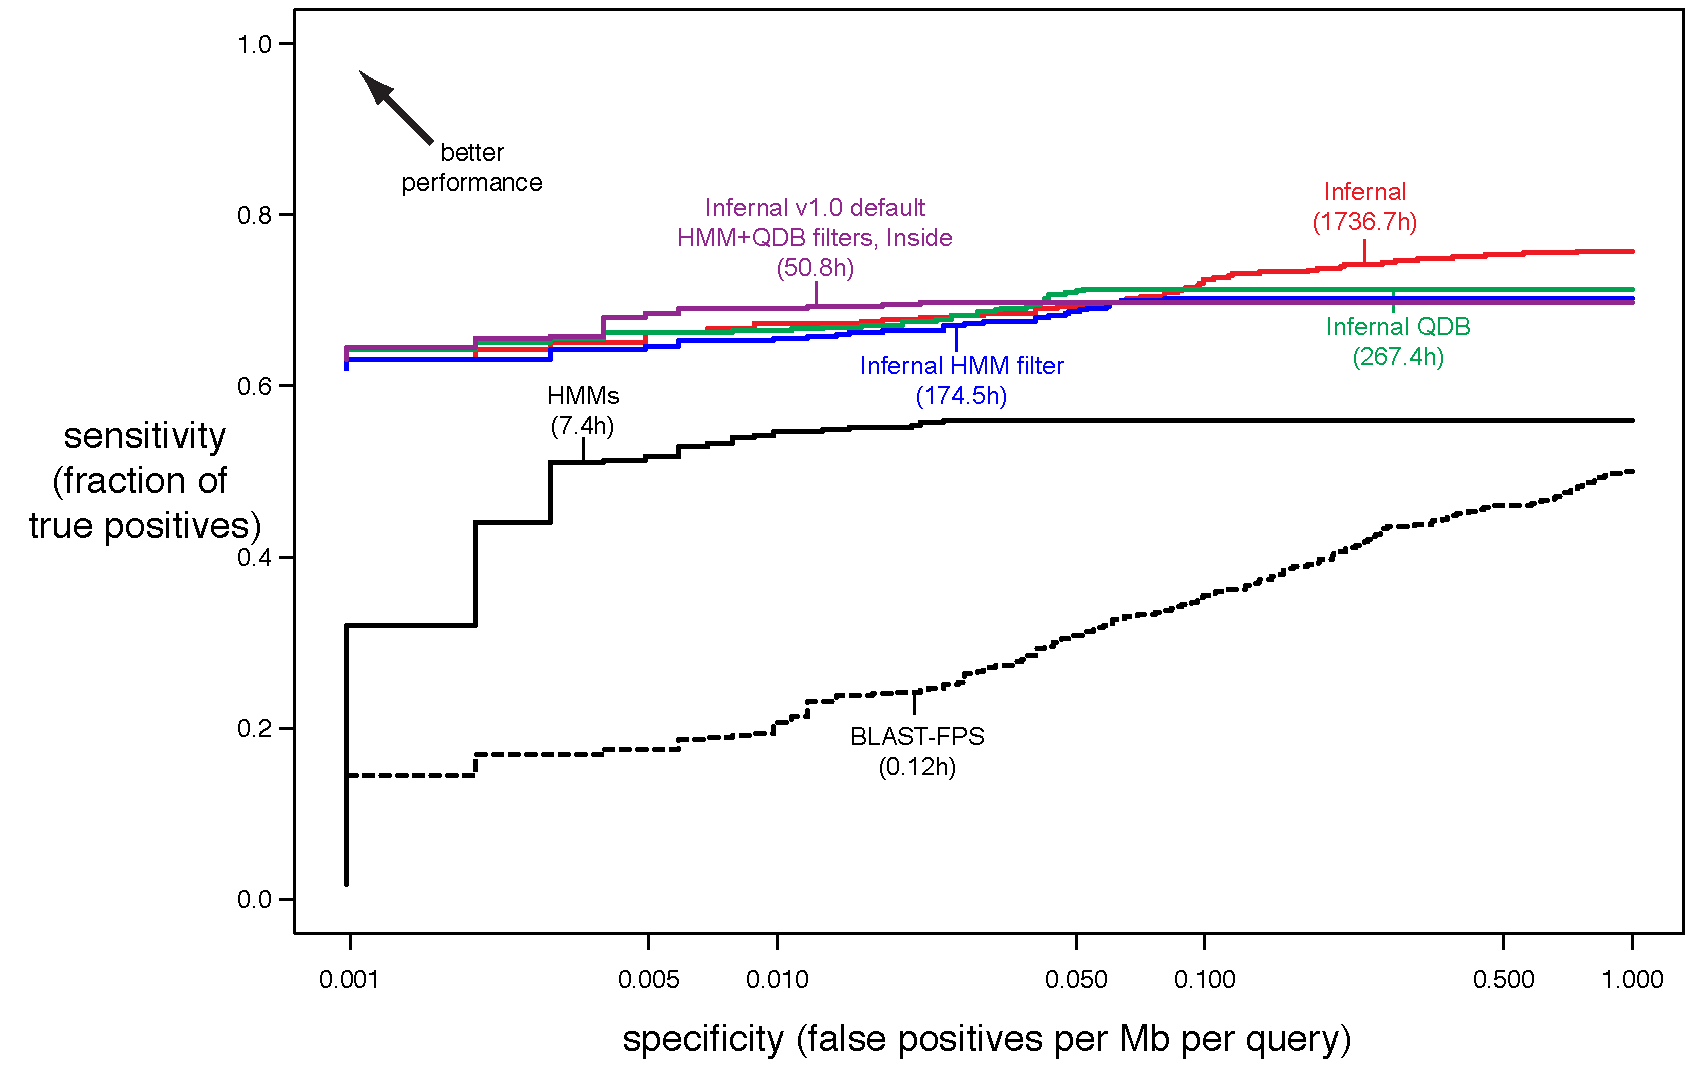
\includegraphics[width=10in]{figs/brown-roc4}}

\vfill 
\end{slide}
%%%%%%%%%%%%%%%%%%%%%%%%%%%%%%%%%%%%%%%%%%%%%%%%%%%%%%%%%%%%%%%%%%%%%%%%%%
\begin{slide}

% BLANK SLIDE TO EMPHASIS BIG SWITCH FROM HOMOLOGY SEARCH TO ALIGNMENT
\textcolor{white}{a}
\vfill

\end{slide}
%%%%%%%%%%%%%%%%%%%%%%%%%%%%%%%%%%%%%%%%%%%%%%%%%%%%%%%%%%%%%%%%%%%%%%%%%%
%%%%%%%%%%    COMMENTED OUT %%%%%%%%%%%%%
\begin{comment}
\begin{slide}
\begin{center}
\small
\textbf{CMs can also be used to create structural alignments of
    homologous RNAs.}
\end{center}
\medskip

\small
\begin{itemize}
%  \item Finding RNAs in an organism's genome is informs us about the
%    organism.
%    Collecting and analyzing many homologous RNAs from different
%    genomes can inform us about the RNA family:
%  \item CMs can also be used to create structural alignments of
%    homologous RNAs.
  \item Given known homologs, place homologous residues in the same columns.
\end{itemize}

\center{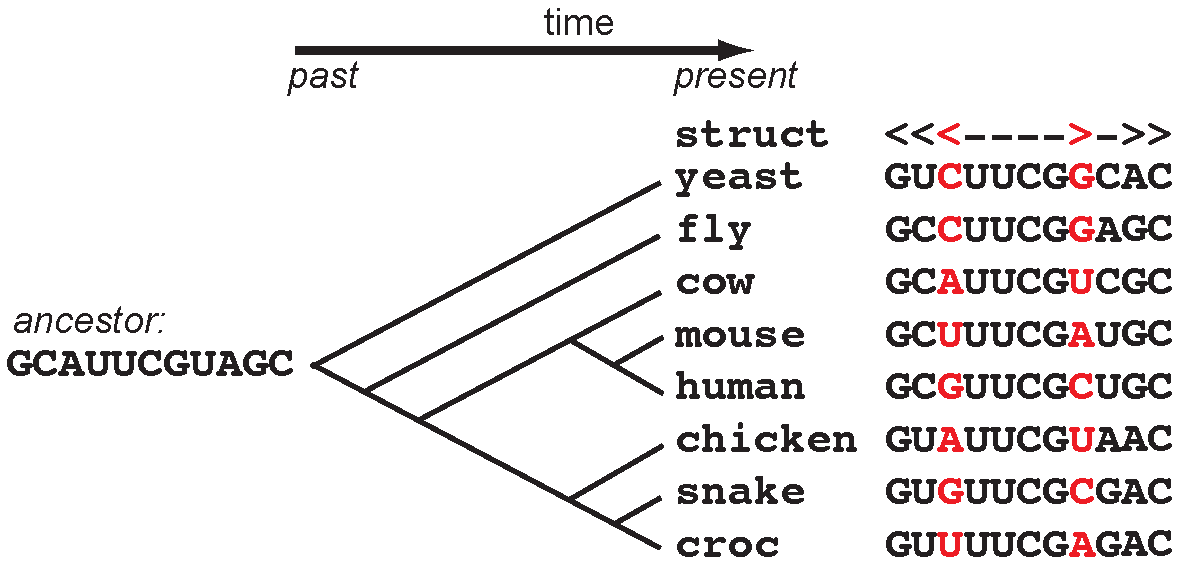
\includegraphics[width=7in]{figs/tree-and-aln}}

\begin{itemize}
\item Alignments of SSU rRNA have commonly been used for phylogenetic inference.

%\begin{itemize}
%  \item RNA alignments have several important applications:
%    \begin{itemize}
%      \item structural inference
%      \item lead to functional hypotheses
%      \item inference of evolutionary history (phylogenetic inference)
%    \end{itemize}
%  \item One RNA in particular has traditionally been used heavily for
%    \\ phylogenetic inference: 

%\item Alignments of SSU rRNA have commonly been used for phylogenetic inference.

\item However, CM alignment is too slow for SSU alignment.
   \\ Aligning a single SSU sequence takes more than 10
    minutes.
\end{itemize}
\vfill
\end{slide}
\end{comment}
%%%%%%%%%%%%    COMMENTED OUT %%%%%%%%%
%%%%%%%%%%%%%%%%%%%%%%%%%%%%%%%%%%%%%%%%%%%%%%%%%%%%%%%%%%%%%%%%%%%%%
\begin{slide}
\begin{center}
\textbf{Small subunit ribosomal RNA and the tree of life}
\end{center}
\medskip
\begin{minipage}{5.2in}
\small

\begin{itemize}
\item 1977 - Carl Woese decided to classify all living things phylogenetically
\item needed ``\emph{a molecule of appropriately broad distribution}'' for comparative analysis
\item SSU rRNA was chosen
\begin{itemize}
  \item universally distributed
  \item highly conserved 
  \item large enough to provide sufficient data (1500-1800 nt)
  \item readily isolated
\end{itemize}
\end{itemize}

\vspace{2.7in}
\end{minipage}
\hspace{0.1in}
\begin{minipage}{5.5in}
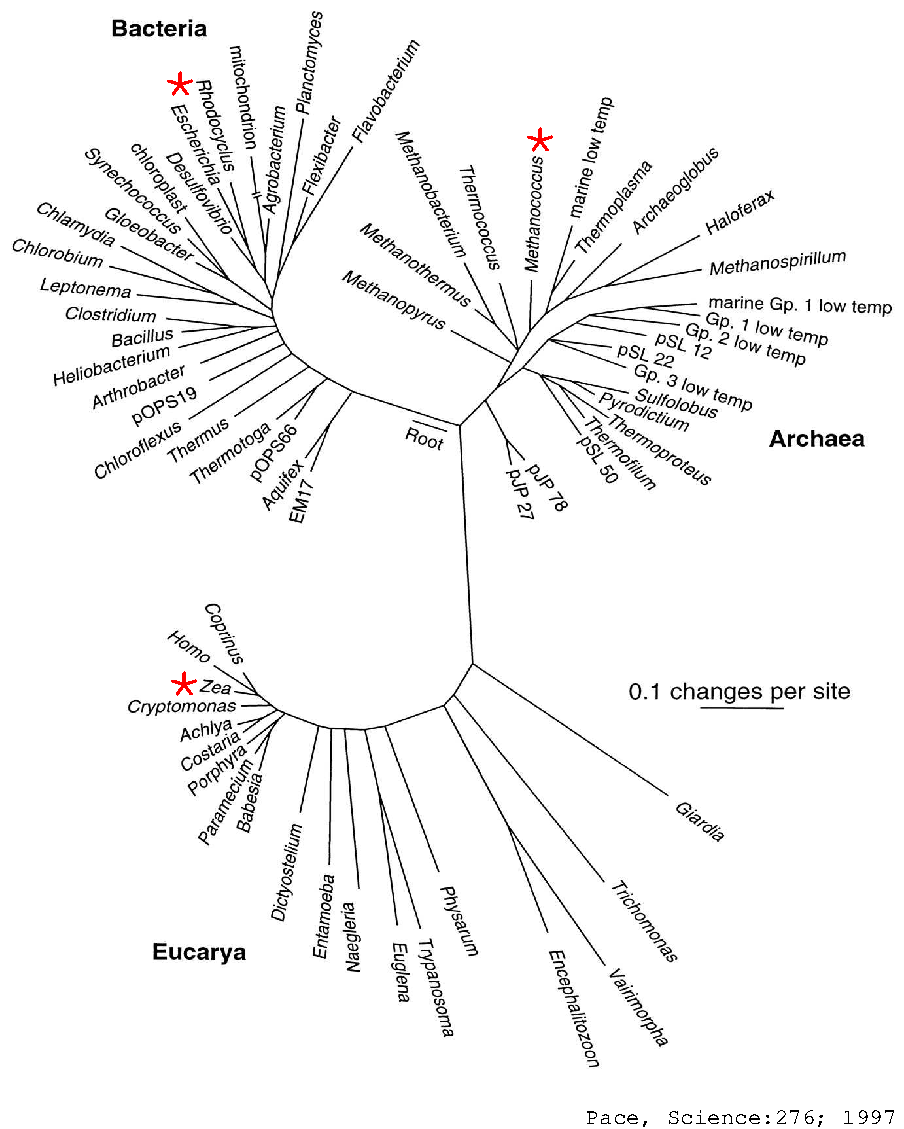
\includegraphics[width=5.5in]{figs/bigtol}
\end{minipage}  
\end{slide}
%%%%%%%%%%%%%%%%%%%%%%%%%%%%%%%%%%%%%%%%%%%%%%%%%%%%%%%%%%%%%%%%%%%%%%%%%%
\begin{slide}
\begin{center}

\textbf{Universal conservation of SSU rRNA}
\end{center}
\vspace{0.5in}
\small
\hspace{0.75in}
\emph{Escherichia coli}
\hspace{1.2in}
\emph{Methanococcus vannielii}
\hspace{1.2in}
\emph{Zea mays}

\begin{center}
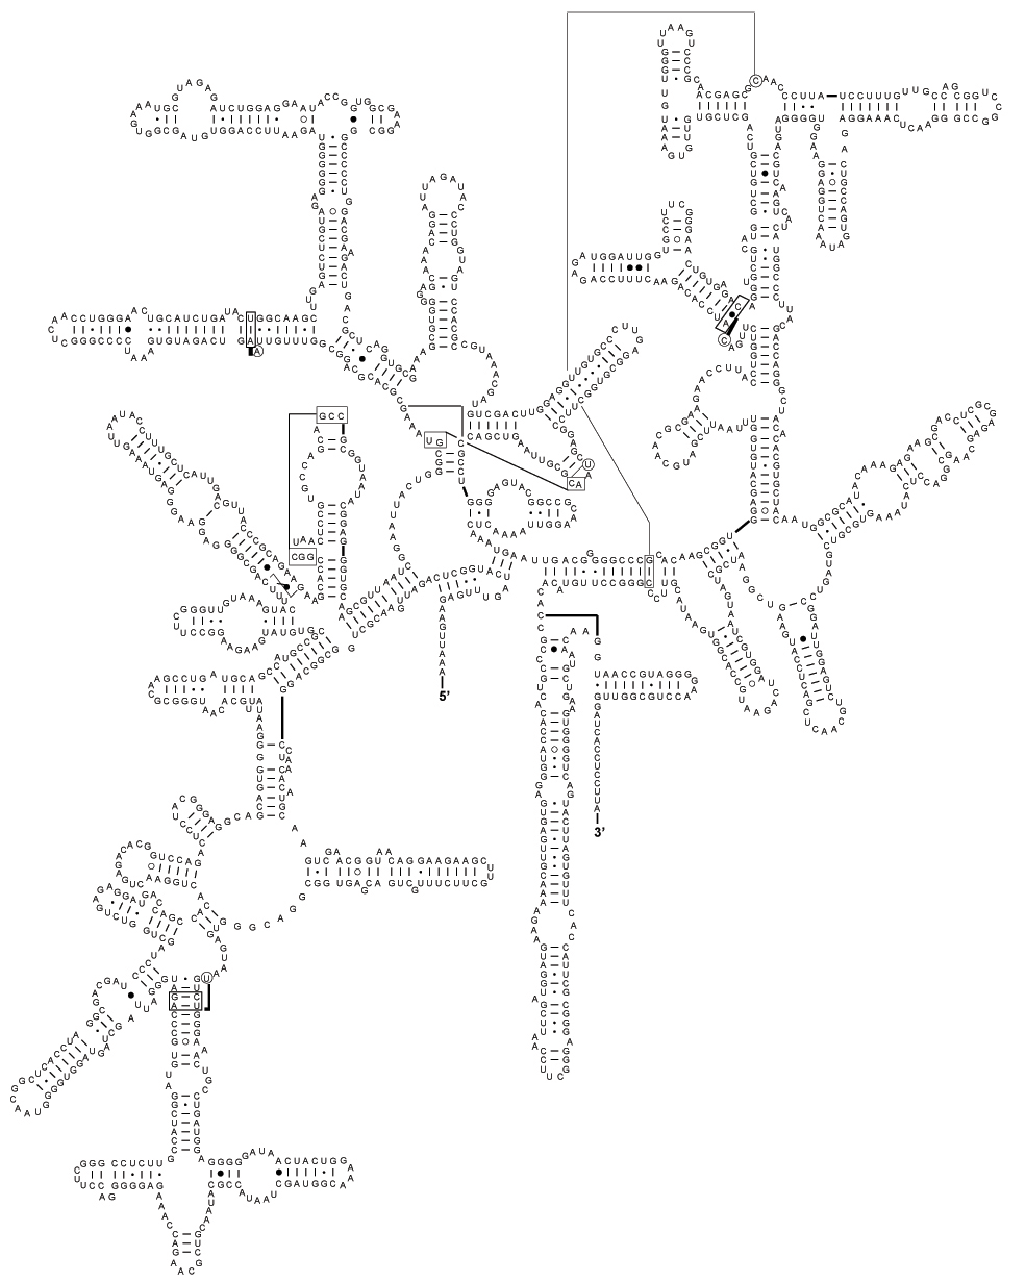
\includegraphics[height=4.45in]{figs/ecoli_16S_man}
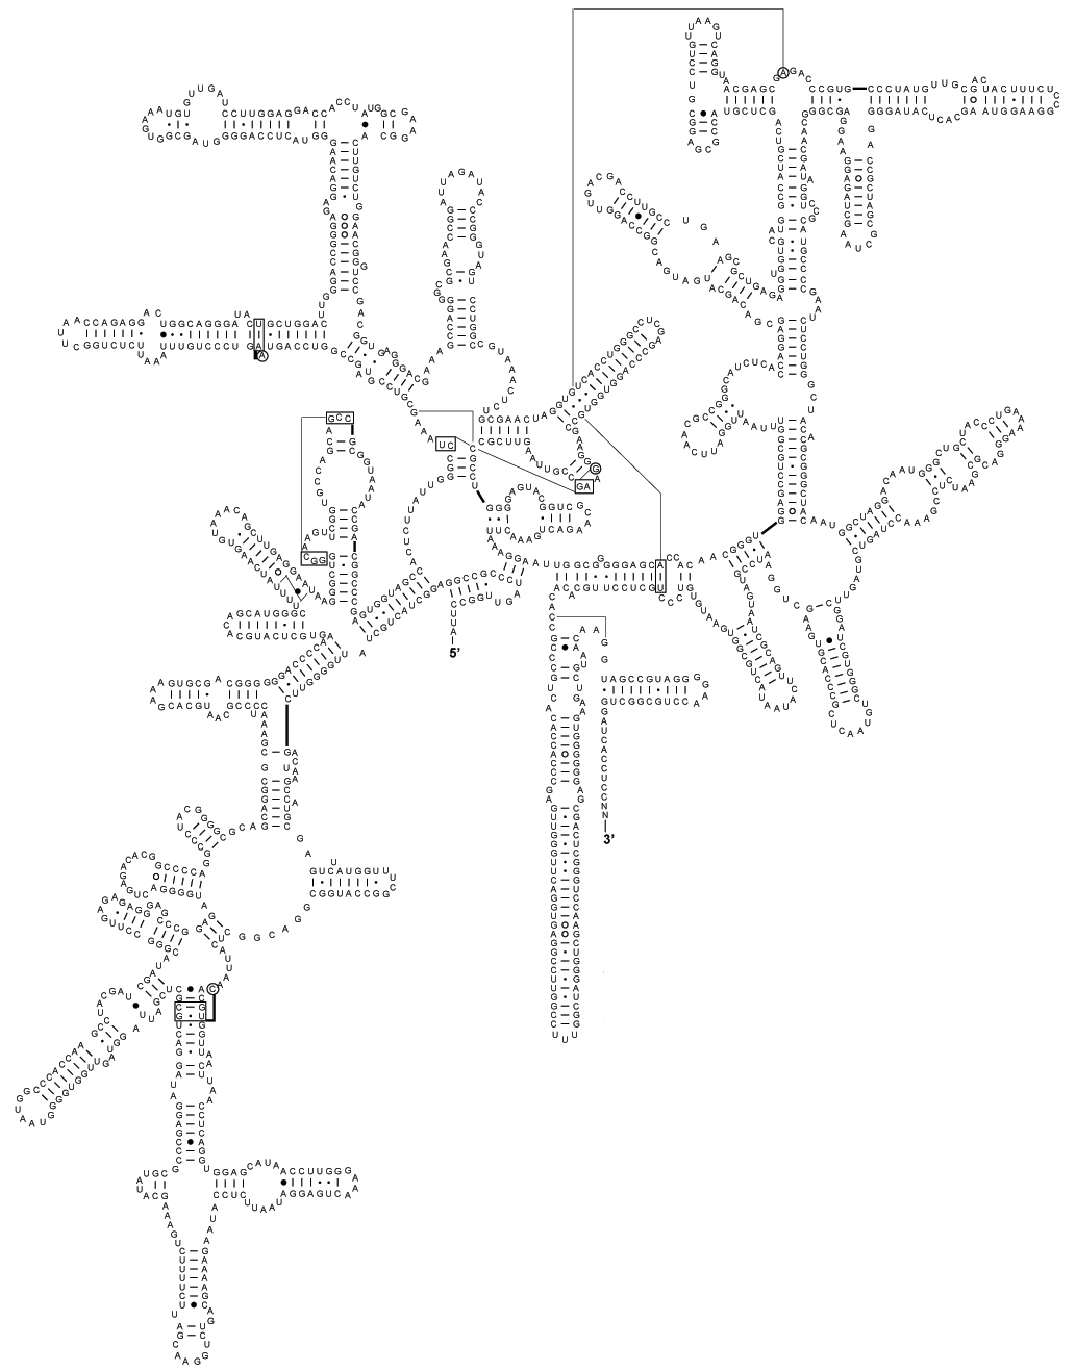
\includegraphics[height=4.45in]{figs/mvan_16S_man}
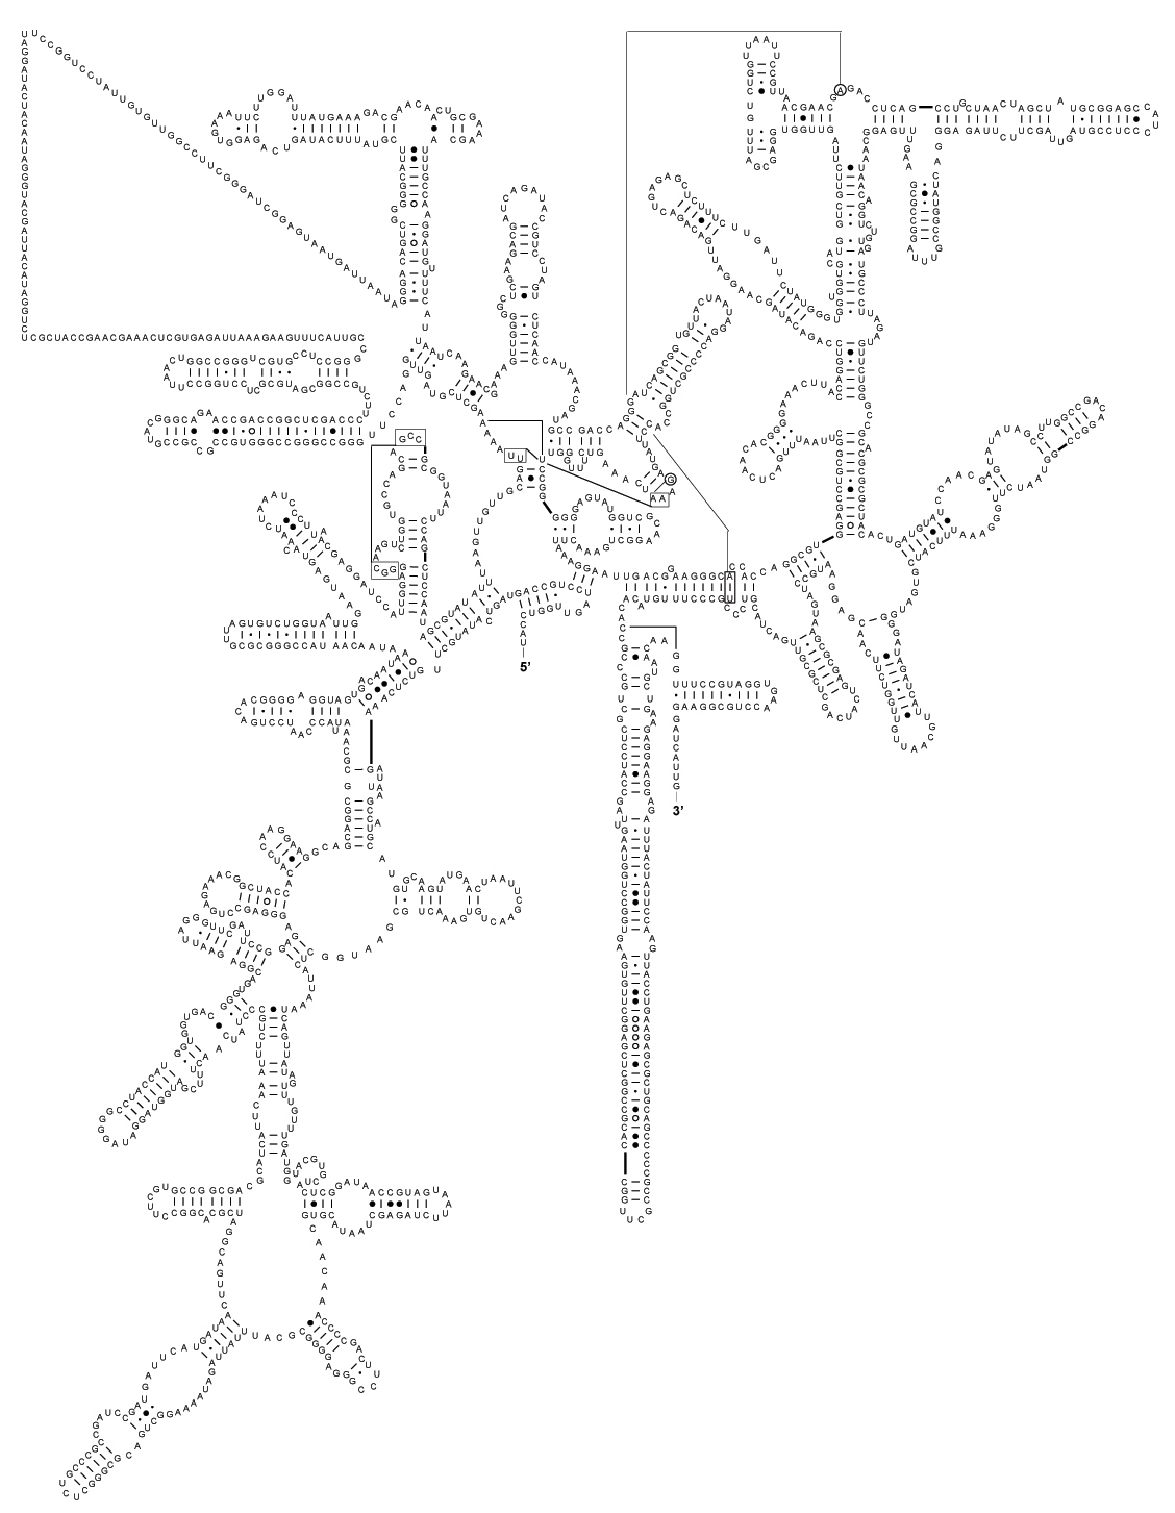
\includegraphics[height=4.45in]{figs/zmays_16S_man}
\end{center}

\begin{flushright}
\tiny{\texttt{Secondary structure diagrams from:}} \\
\tiny{\texttt{URL:http://www.rna.ccbb.utexas.edu/}}
\end{flushright}
\vfill
\end{slide}
%%%%%%%%%%%%%%%%%%%%%%%%%%%%%%%%%%%%%%%%%%%%%%%%%%%%%%%%%%%%%%%%%%%%%%%%%%
\begin{slide}
\begin{center}
\textbf{Sequence conservation in SSU rRNA}
\end{center}
\vspace{0.5in}
\small
\hspace{1.5in}
\underline{bacteria}
\hspace{2.2in}
\underline{archaea}
\hspace{2.2in}
\underline{eukarya}

\begin{center}
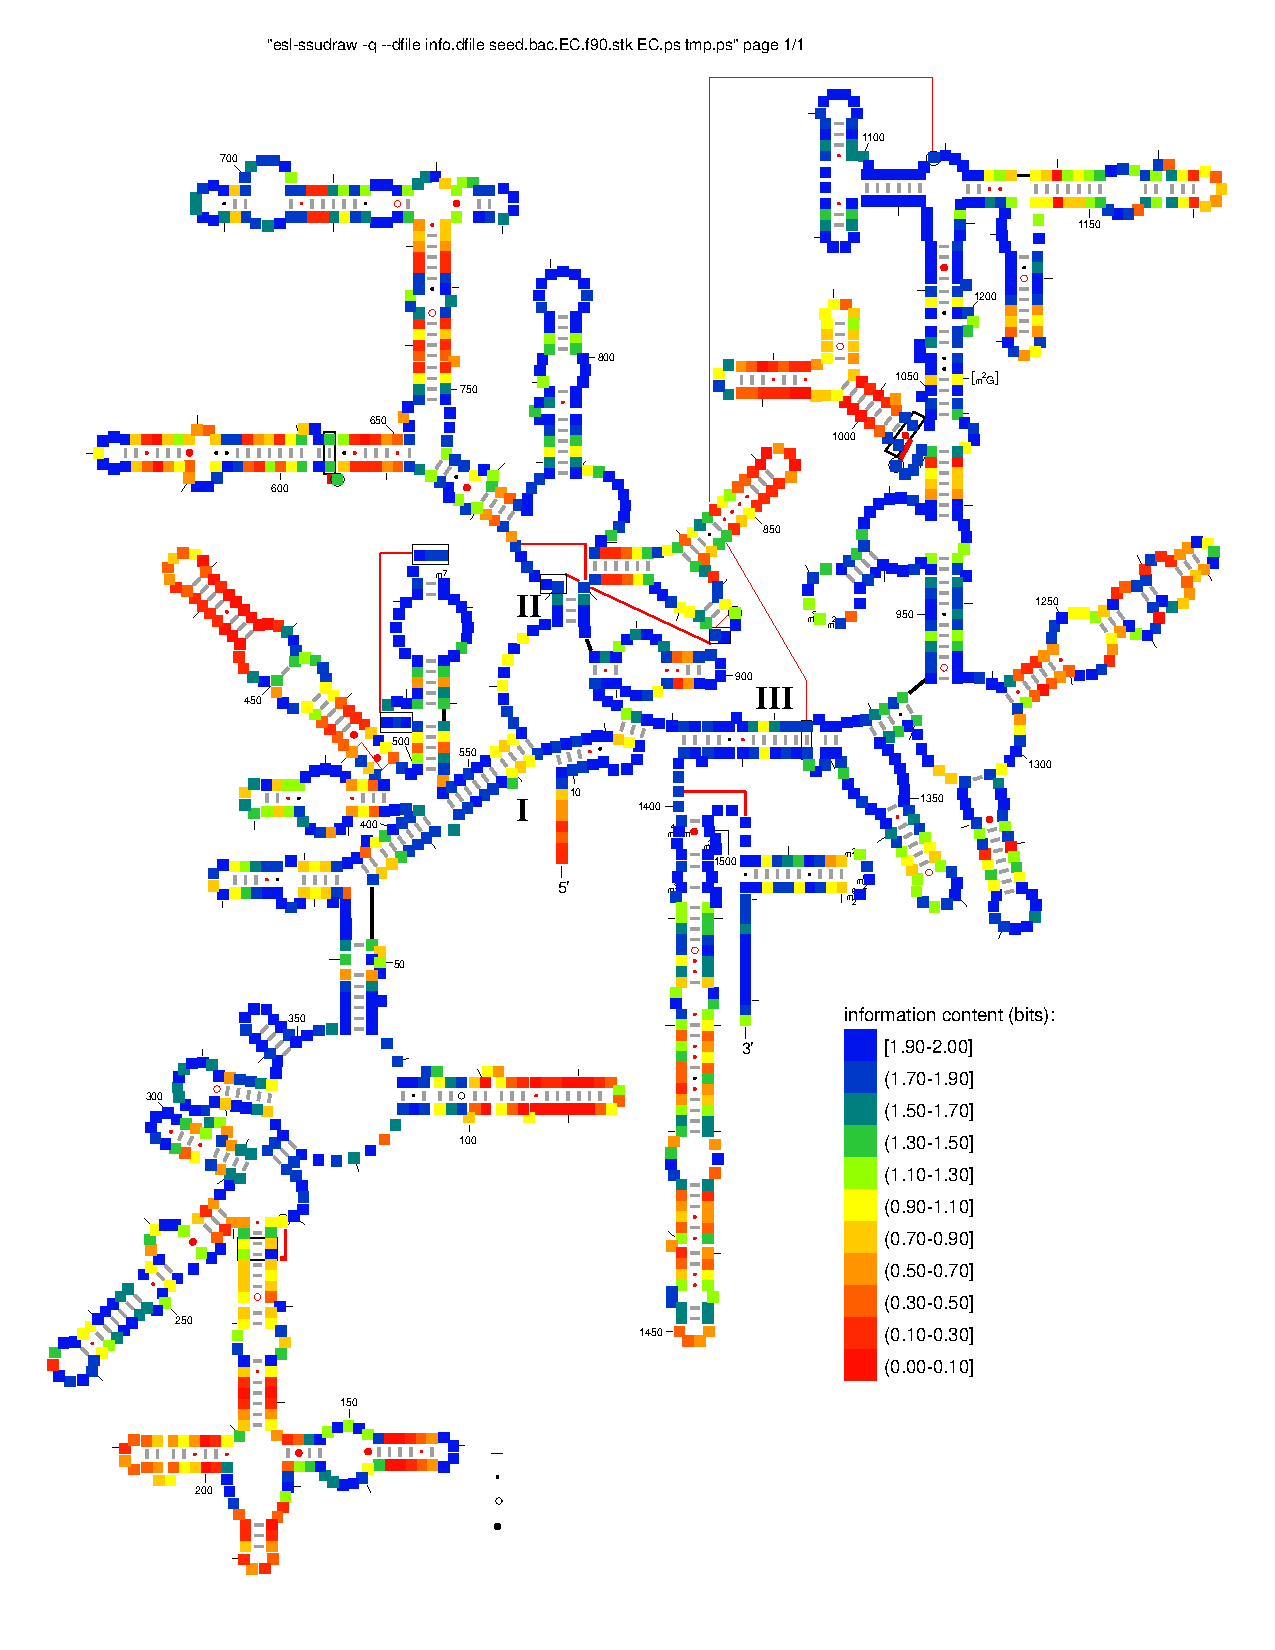
\includegraphics[height=4.45in]{figs/bac_info_heat}
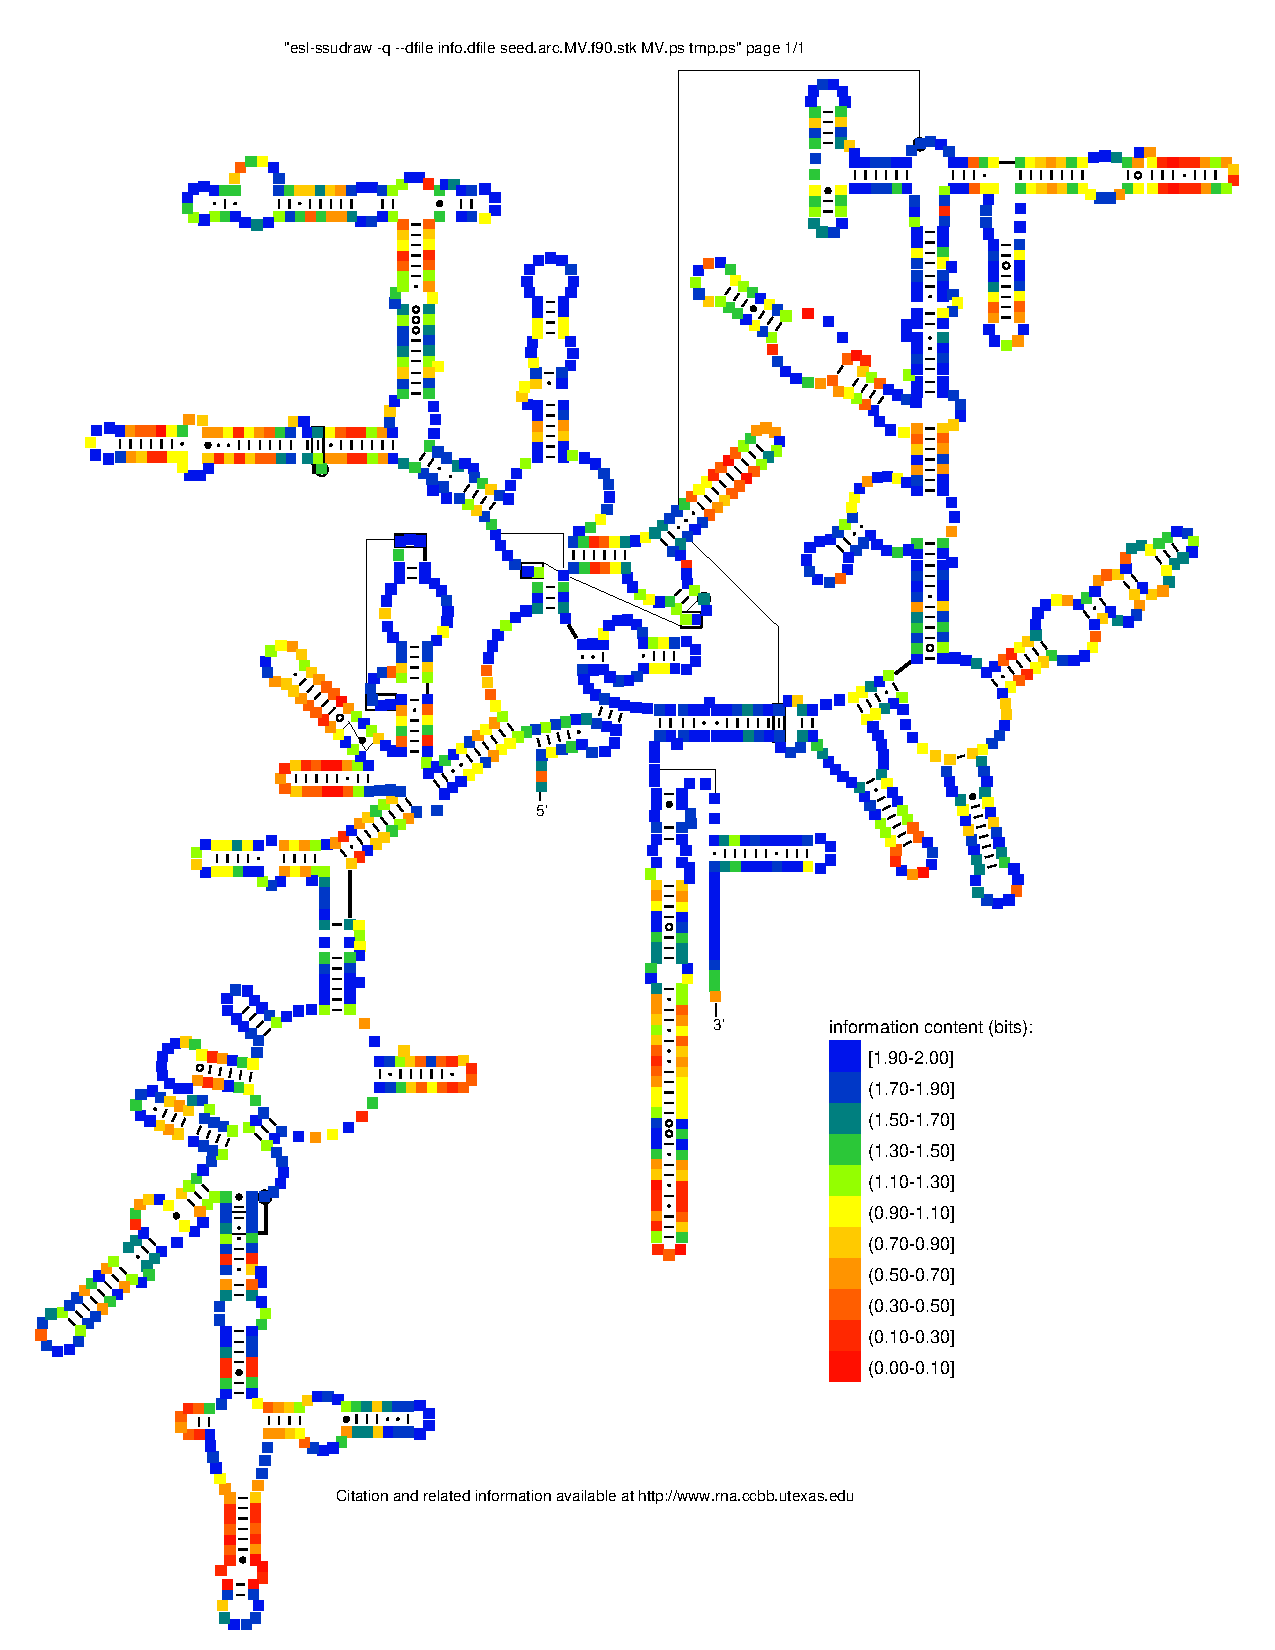
\includegraphics[height=4.45in]{figs/arc_info_heat}
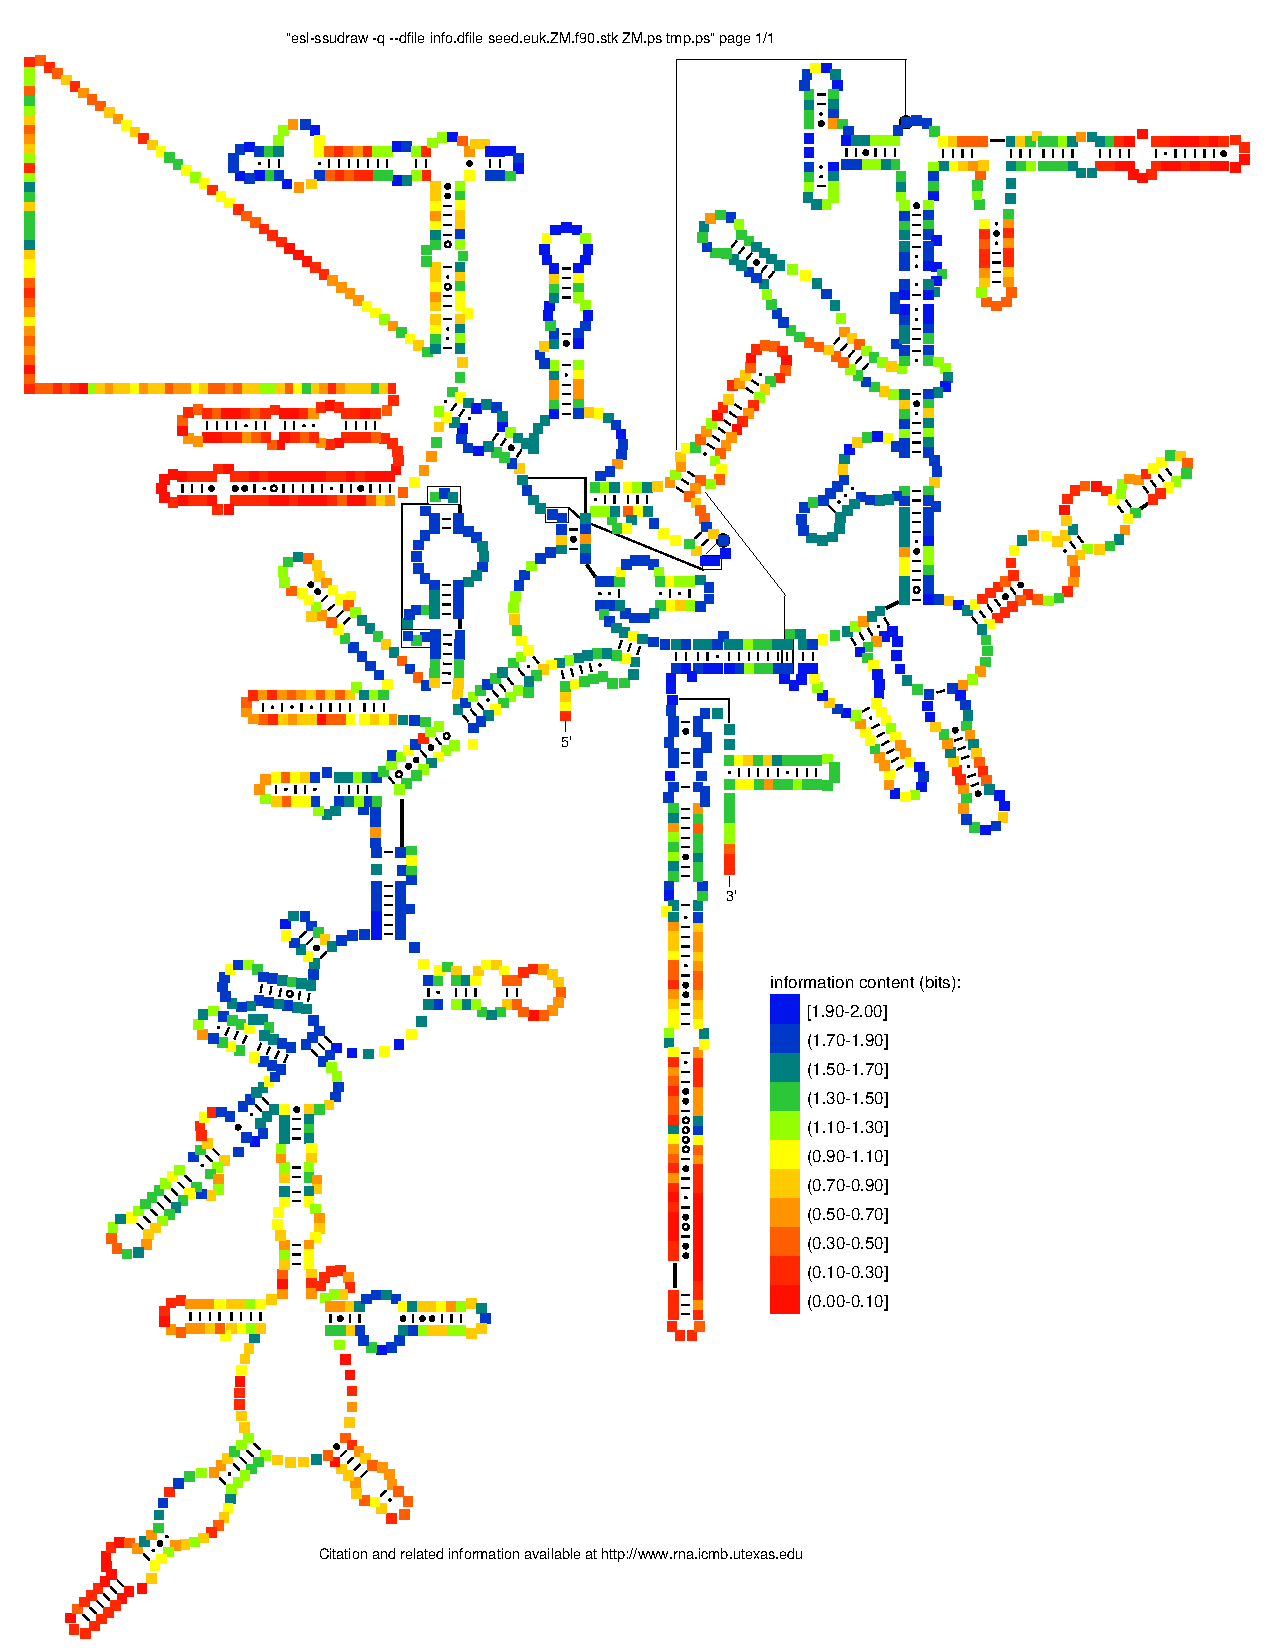
\includegraphics[height=4.45in]{figs/euk_info_heat}
\end{center}

\begin{flushright}
\tiny{\texttt{Secondary structure diagrams created based}} \\
\tiny{\texttt{alignments and diagrams from:}} \\
\tiny{\texttt{URL:http://www.rna.ccbb.utexas.edu/}}
\end{flushright}
\vfill
\end{slide}
%%%%%%%%%%%%%%%%%%%%%%%%%%%%%%%%%%%%%%%%%%%%%%%%%%%%%%%%%%%%%%%%%%%%%%%%%%
\begin{slide}
\begin{center}

\textbf{Environmental surveys target SSU}
\end{center}
\medskip
\begin{minipage}{7in}
\small
\begin{itemize}
\item mid 1980s - Norman Pace develops methodology for determination
      of SSU sequences without cultivation
\item many different environments have been surveyed
\item known biodiversity has been greatly expanded:

\begin{itemize}
\item
  recognized bacterial phyla: \\
  11 in 1987, 36 in 1998, 52 in 2003, 67 in 2006...
\end{itemize}

\item SSU databases contain millions of sequences:
\begin{center}
\begin{tabular}{lrr}
  name & \# seqs & \# citations \\ \hline
  Silva & 4.4M & 1972 \\ 
  RDP   & 2.9M & 2150 \\
  Greengenes & 1.0M & 1635 \\
\end{tabular}
\end{center}
\end{itemize}

\tiny
Silva: Pruesse et al., 2007 NAR 35.21:7188-96 \\
RDP: Cole et al., 2009 NAR 37:D141-45 \\
Greengenes: DeSantis et al., 2006 AEM 72:5069-72 \\

\vspace{1.6in}
\end{minipage}
\hspace{0.1in}
\begin{minipage}{3in}
\includegraphics[height=6in]{figs/environmental}
\vspace{1in}
\end{minipage}
\end{slide}

%%%%%%%%%%%%%%%%%%%%%%%%%%%%%%%%%%%%%%%%%%%%%%%%%%%%%%%%%%%%%%%%%%%%%%%%%%
\begin{slide}
\begin{center}

%\large
\textbf{The comparative analysis step: \\ \textcolor{red}{Alignment} and Phylogenetic Inference}
\end{center}

\center{\includegraphics[height=7in]{figs/seq2tree}}
%\center{\includegraphics[height=7in]{figs/ssu_list_and_seq2tree_masked}}
\vfill
\end{slide}
%%%%%%%%%%%%%%%%%%%%%%%%%%%%%%%%%%%%%%%%%%%%%%%%%%%%%%%%%%%%%%%%%%%%%%%%%%
%%%%%%%%%%%%COMMENTED OUT%%%%%%%%%%%%%%%%%%%%%%%%%%%%%%%%%%%%%%%%%%%%%%%%%
\begin{comment}
\begin{slide}
\begin{center}

\textbf{Environmental surveys target SSU rRNA}
\end{center}

%\includegraphics[height=6in]{figs/ssu_gb_surveys_list_2007}
\center{\includegraphics[height=7in]{figs/ssu_list_and_seq2tree_blackgrey}}
%\center{\includegraphics[height=7in]{figs/ssu_list_and_seq2tree_bluegold}}
\vfill
\end{slide}
\end{comment}
%%%%%%%%%%%%COMMENTED OUT%%%%%%%%%%%%%%%%%%%%%%%%%%%%%%%%%%%%%%%%%%%%%%%%%
%%%%%%%%%%%%%%%%%%%%%%%%%%%%%%%%%%%%%%%%%%%%%%%%%%%%%%%%%%%%%%%%%%%%%%%%%%
\begin{slide}
\begin{center}

\textbf{Accelerating CM alignment using HMMs}
\end{center}
\medskip
\begin{minipage}{6in}
\footnotesize
\begin{itemize}
\item
\textbf{main idea:} use fast HMM when it's accurate, appealing to CM when it's not
\item
need some type of measure of confidence in regions of the HMM alignment

\end{itemize}
\small
\hspace{0.3in}
\underline{HMM alignment}%\hspace{1.5in}---- $>$
\begin{itemize}

\item
each column of the grid corresponds to a \\ column
of the seed alignment
\item
each row of the grid corresponds to a \\ position of the new sequence
\end{itemize}
\vspace{3in}
\end{minipage}
\begin{minipage}{4in}
\begin{center}
\includegraphics[height=6in]{figs/hmm_alignment2_layer1}
\end{center}
\vspace{1.5in}
\end{minipage}
\end{slide}
%%%%%%%%%%%%%%%%%%%%%%%%%%%%%%%%%%%%%
%%%%%%%%%%%%%%%%%%%%%%%%%%%%%%%%%%%%%%%%%%%%%%%%%%%%%%%%%%%%%%%%%%%%%%%%%%
\begin{slide}
\begin{center}

\textbf{Accelerating CM alignment using HMMs}
\end{center}
\medskip
\begin{minipage}{6in}
\footnotesize
\begin{itemize}
\item
\textbf{main idea:} use fast HMM when it's accurate, appealing to CM when it's not
\item
need some type of measure of confidence in regions of the HMM alignment

\end{itemize}
\small
\hspace{0.3in}
\underline{HMM alignment}%\hspace{1.5in}---- $>$
\begin{itemize}
\item
each column of the grid corresponds to a \\ column
of the seed alignment
\item
each row of the grid corresponds to a \\ position of the new sequence
\end{itemize}
\vspace{3in}
\end{minipage}
\begin{minipage}{4in}
\begin{center}
\includegraphics[height=6in]{figs/hmm_alignment2_layer2}
\end{center}
\vspace{1.5in}
\end{minipage}
\end{slide}
%%%%%%%%%%%%%%%%%%%%%%%%%%%%%%%%%%%%%
%%%%%%%%%%%%%%%%%%%%%%%%%%%%%%%%%%%%%%%%%%%%%%%%%%%%%%%%%%%%%%%%%%%%%%%%%%
\begin{slide}
\begin{center}

\textbf{Accelerating CM alignment using HMMs}
\end{center}
\medskip
\begin{minipage}{6in}
\footnotesize
\begin{itemize}
\item
\textbf{main idea:} use fast HMM when it's accurate, appealing to CM when it's not
\item
need some type of measure of confidence in regions of the HMM alignment

\end{itemize}
\small
\hspace{0.3in}
\underline{HMM alignment}%\hspace{1.5in}---- $>$
\begin{itemize}
\item
each column of the grid corresponds to a \\ column
of the seed alignment
\item
each row of the grid corresponds to a \\ position of the new sequence
\end{itemize}
\begin{center}
\normalsize
\textbf{How can we use this information during CM alignment?}
\end{center}
\vspace{1.9in}
\end{minipage}
\begin{minipage}{4in}
\begin{center}
\includegraphics[height=6in]{figs/hmm_alignment2_layer3}
\end{center}
\vspace{1.5in}
\end{minipage}
\end{slide}
%%%%%%%%%%%%%%%%%%%%%%%%%%%%%%%%%%%%%
\begin{slide}
\begin{center}

\textbf{HMM bands accelerate CM alignment}
\end{center}
\medskip
\small
\begin{itemize}
\item
\textbf{main idea:} eliminate potential alignments the HMM tells us are very improbable
\end{itemize}
\begin{center}
\includegraphics[width=8in]{figs/post_hmm_to_cm_map2_layer10}
\end{center}
\vfill
\end{slide}
%%%%%%%%%%%%%%%%%%%%%%%%%%%%%%%%%%%%%%%%%%%%%%%%%%%%%%%%%%%%%%%%%%%%%%%%%%
%%%%%%%%%%%%%%%%%%%%%%%%%%%%%%%%%%%%%%%%%%%%%%%%%%%%%%%%%%%%%%%%%%%%%%%%%%
\begin{slide}
\begin{center}

\textbf{HMM bands accelerate CM alignment}
\end{center}
\medskip
\small
\begin{itemize}
\item
\textbf{main idea:} eliminate potential alignments the HMM tells us are very improbable
\end{itemize}
\begin{center}
\includegraphics[width=8in]{figs/post_hmm_to_cm_map2_layer11}
\end{center}
\vfill
\end{slide}
%%%%%%%%%%%%%%%%%%%%%%%%%%%%%%%%%%%%%%%%%%%%%%%%%%%%%%%%%%%%%%%%%%%%%%%%%%
%%%%%%%%%%%%%%%%%%%%%%%%%%%%%%%%%%%%%%%%%%%%%%%%%%%%%%%%%%%%%%%%%%%%%%%%%%
\begin{slide}
\begin{center}

\textbf{HMM bands accelerate CM alignment}
\end{center}
\medskip
\small
\begin{itemize}
\item
\textbf{main idea:} eliminate potential alignments the HMM tells us are very improbable
\end{itemize}
\begin{center}
\includegraphics[width=8in]{figs/post_hmm_to_cm_map2_layer12}
\end{center}
\vfill
\end{slide}
%%%%%%%%%%%%%%%%%%%%%%%%%%%%%%%%%%%%%%%%%%%%%%%%%%%%%%%%%%%%%%%%%%%%%%%%%%
%%%%%%%%%%%%%%%%%%%%%%%%%%%%%%%%%%%%%%%%%%%%%%%%%%%%%%%%%%%%%%%%%%%%%%%%%%
\begin{slide}
\begin{center}

\textbf{HMM bands accelerate CM alignment}
\end{center}
\medskip
\small
\begin{itemize}
\item
\textbf{main idea:} eliminate potential alignments the HMM tells us are very improbable
\end{itemize}
\begin{center}
\includegraphics[width=8in]{figs/post_hmm_to_cm_map2_layer13}
\end{center}
\vfill
\end{slide}
%%%%%%%%%%%%%%%%%%%%%%%%%%%%%%%%%%%%%%%%%%%%%%%%%%%%%%%%%%%%%%%%%%%%%%%%%%
%%%%%%%%%%%%%%%%%%%%%%%%%%%%%%%%%%%%%%%%%%%%%%%%%%%%%%%%%%%%%%%%%%%%%%%%%%
\begin{slide}
\begin{center}

\textbf{HMM bands accelerate CM alignment}
\end{center}
\medskip
\small
\begin{itemize}
\item
\textbf{main idea:} eliminate potential alignments the HMM tells us are very improbable
\end{itemize}
\begin{center}
\includegraphics[width=8in]{figs/post_hmm_to_cm_map2_layer14}
\end{center}
\vfill
\end{slide}
%%%%%%%%%%%%%%%%%%%%%%%%%%%%%%%%%%%%%%%%%%%%%%%%%%%%%%%%%%%%%%%%%%%%%%%%%%
%%%%%%%%%%%%%%%%%%%%%%%%%%%%%%%%%%%%%%%%%%%%%%%%%%%%%%%%%%%%%%%%%%%%%%%%%%
\begin{slide}
\begin{center}

\textbf{HMM bands accelerate CM alignment}
\end{center}
\medskip
\small
\begin{itemize}
\item
\textbf{main idea:} eliminate potential alignments the HMM tells us are very improbable
\end{itemize}
\begin{center}
\includegraphics[width=8in]{figs/post_hmm_to_cm_map2_layer15}
\end{center}
\vfill
\end{slide}
%%%%%%%%%%%%%%%%%%%%%%%%%%%%%%%%%%%%%%%%%%%%%%%%%%%%%%%%%%%%%%%%%%%%%%%%%%
%%%%%%%%%%%%%%%%%%%%%%%%%%%%%%%%%%%%%%%%%%%%%%%%%%%%%%%%%%%%%%%%%%%%%%%%%%
\begin{slide}
\begin{center}

\textbf{HMM bands accelerate CM alignment}
\end{center}
\medskip
\small
\begin{itemize}
\item
\textbf{main idea:} eliminate potential alignments the HMM tells us are very improbable
\end{itemize}
\begin{center}
\includegraphics[width=8in]{figs/post_hmm_to_cm_map2_layer16}
\end{center}
\vfill
\end{slide}
%%%%%%%%%%%%%%%%%%%%%%%%%%%%%%%%%%%%%%%%%%%%%%%%%%%%%%%%%%%%%%%%%%%
\begin{slide}
\begin{center}

\textbf{Determining the impact of HMM banding on speed and accuracy}
\end{center}
\medskip

\small
\begin{itemize}
%\item
%Does the banded CM approach 
%sacrifice accuracy relative to
%non-banded CM alignment?
\item
'Gold standard' testing dataset
\begin{itemize}
\item
structural alignment of 152 bacterial SSU sequences
from Robin Gutell's database
%\item
%this is the CRW bacterial seed alignment filtered to 92\% identity
\item
determined by 'manual' comparative analysis

\end{itemize}
\end{itemize}

%\center{\includegraphics[width=10.5in]{figs/diana_benchmark_l1}}
\center{\includegraphics[width=10.5in]{figs/diana_benchmark_l2}}

\vfill
\end{slide}
%%%%%%%%%%%%%%%%%%%%%%%%%%%%%%%%%%%%%%%%%%%%%%%%%%%%%%%%%%%%%%%%%%%%%%%%%
%%%%%%%%%%%%%%%%%%%%%%%%%%%%%%%%%%%%%%%%%%%%%%%%%%%%%%%%%%%%%%%%%%%%%%%%%
\begin{slide}
\begin{center}

\textbf{CMs are (slightly) more accurate, but much slower than HMMs}
\end{center}
\medskip
\medskip
\begin{center}

\begin{tabular}{rcr} 
& \multicolumn{1}{c}{alignment} & \multicolumn{1}{c}{time} \\
& \multicolumn{1}{c}{accuracy} & \multicolumn{1}{c}{(sec/seq)} \\ \hline
& \multicolumn{1}{c}{} & \multicolumn{1}{c}{} \\
Muscle-3.8.31 (\emph{de novo}) & 95.4\% & 0.49 \\
& \multicolumn{1}{c}{} & \multicolumn{1}{c}{} \\
HMMER3 (HMMs) & 96.8\% & 0.04 \\ 
& \multicolumn{1}{c}{} & \multicolumn{1}{c}{} \\
non-banded CMs & 98.1\% & 276.76 \\
& \multicolumn{1}{c}{} & \multicolumn{1}{c}{} \\
%HMM banded CMs & 98.1\% & 0.7 \\ %1.1
%& \multicolumn{1}{c}{} & \multicolumn{1}{c}{} \\
\end{tabular}
\end{center}

\vfill
\scriptsize
\flushright{Muscle: Edgar, R.C. Nucleic Acids Res 32(5), 1792-97.}
\flushright{HMMER: hmmer.janelia.org}
\flushright{Infernal: infernal.janelia.org}
\end{slide}
%%%%%%%%%%%%%%%%%%%%%%%%%%%%%%%%%%%%%%%%%%%%%
%%%%%%%%%%%%%%%%%%%%%%%%%%%%%%%%%%%%%%%%%%%%%%%%%%%%%%%%%%%%%%%%%%%%%%%%%
\begin{slide}
\begin{center}

\textbf{HMM banding accelerates CM alignment 500-fold}
\end{center}
\medskip
\medskip
\begin{center}

\begin{tabular}{rcr} 
& \multicolumn{1}{c}{alignment} & \multicolumn{1}{c}{time} \\
& \multicolumn{1}{c}{accuracy} & \multicolumn{1}{c}{(sec/seq)} \\ \hline
& \multicolumn{1}{c}{} & \multicolumn{1}{c}{} \\
Muscle-3.8.31 (\emph{de novo}) & 95.4\% & 0.49 \\
& \multicolumn{1}{c}{} & \multicolumn{1}{c}{} \\
HMMER3 (HMMs) & 96.8\% & 0.04 \\ 
& \multicolumn{1}{c}{} & \multicolumn{1}{c}{} \\
non-banded CMs & 98.1\% & 276.76 \\
& \multicolumn{1}{c}{} & \multicolumn{1}{c}{} \\
HMM banded CMs & 98.1\% & 0.50 \\ %1.1
& \multicolumn{1}{c}{} & \multicolumn{1}{c}{} \\
\end{tabular}
\end{center}

\vfill
\scriptsize
\flushright{Muscle: Edgar, R.C. Nucleic Acids Res 32(5), 1792-97.}
\flushright{HMMER: hmmer.janelia.org}
\flushright{Infernal: infernal.janelia.org}
\end{slide}
%%%%%%%%%%%%%%%%%%%%%%%%%%%%%%%%%%%%%%%%%%%%%%%%%%%%%%%%%%%%%%%%%%%%%%%%%
\begin{slide}
\begin{center}
\textbf{SSU analyses commonly mask (remove) columns \\ from alignment
  prior to phylogenetic inference}
\end{center}

%\center{\includegraphics[height=5in]{figs/seq2tree-2013-thin-mask}}
\center{\includegraphics[height=7in]{figs/seq2tree-2014}}

\vfill
\end{slide}
%%%%%%%%%%%%%%%%%%%%%%%%%%%%%%%%%%%%%%%%%%%%%%%%%%%%%%%%%%%%%%%%%%%%%%%%%%
\begin{slide}
%\begin{center}
%
%\textbf{Phil Hugenholtz's manually created mask}
%\end{center}
%\small
\begin{center}
\includegraphics[height=8in]{figs/archaea-mask-ph-only}

\end{center}
\vfill
\end{slide}
%%%%%%%%%%%%%%%%%%%%%%%%%%%%%%%%%%%%%%%%%%%%%%%%%%%%%%%%%%%%%%%%%%%%%%%%%%%%%%%%%%%%%%%%%%%%%
\begin{slide}\begin{center}\includegraphics[height=8in]{figs/arc-1}\end{center}\vfill\end{slide}
%%%%%%%%%%%%%%%%%%%%%%%%%%%%%%%%%%%%%%%%%%%%%%%%%%%%%%%%%%%%%%%%%%%%%%%%%%%%%%%%%%%%%%%%%%%%%
\begin{slide}\begin{center}\includegraphics[height=8in]{figs/arc-2}\end{center}\vfill\end{slide}
%%%%%%%%%%%%%%%%%%%%%%%%%%%%%%%%%%%%%%%%%%%%%%%%%%%%%%%%%%%%%%%%%%%%%%%%%%%%%%%%%%%%%%%%%%%%%
%\begin{slide}\begin{center}\includegraphics[height=8in]{figs/arc-3}\end{center}\vfill\end{slide}
%%%%%%%%%%%%%%%%%%%%%%%%%%%%%%%%%%%%%%%%%%%%%%%%%%%%%%%%%%%%%%%%%%%%%%%%%%%%%%%%%%%%%%%%%%%%%
%\begin{slide}\begin{center}\includegraphics[height=8in]{figs/arc-4}\end{center}\vfill\end{slide}
%%%%%%%%%%%%%%%%%%%%%%%%%%%%%%%%%%%%%%%%%%%%%%%%%%%%%%%%%%%%%%%%%%%%%%%%%%%%%%%%%%%%%%%%%%%%%
%\begin{slide}\begin{center}\includegraphics[height=8in]{figs/arc-5}\end{center}\vfill\end{slide}
%%%%%%%%%%%%%%%%%%%%%%%%%%%%%%%%%%%%%%%%%%%%%%%%%%%%%%%%%%%%%%%%%%%%%%%%%%%%%%%%%%%%%%%%%%%%%
%\begin{slide}\begin{center}\includegraphics[height=8in]{figs/arc-6}\end{center}\vfill\end{slide}
%%%%%%%%%%%%%%%%%%%%%%%%%%%%%%%%%%%%%%%%%%%%%%%%%%%%%%%%%%%%%%%%%%%%%%%%%%%%%%%%%%%%%%%%%%%%%
%\begin{slide}\begin{center}\includegraphics[height=8in]{figs/arc-7}\end{center}\vfill\end{slide}
%%%%%%%%%%%%%%%%%%%%%%%%%%%%%%%%%%%%%%%%%%%%%%%%%%%%%%%%%%%%%%%%%%%%%%%%%%%%%%%%%%%%%%%%%%%%%
%\begin{slide}\begin{center}\includegraphics[height=8in]{figs/arc-8}\end{center}\vfill\end{slide}
%%%%%%%%%%%%%%%%%%%%%%%%%%%%%%%%%%%%%%%%%%%%%%%%%%%%%%%%%%%%%%%%%%%%%%%%%%%%%%%%%%%%%%%%%%%%%
%\begin{slide}\begin{center}\includegraphics[height=8in]{figs/arc-9}\end{center}\vfill\end{slide}
%%%%%%%%%%%%%%%%%%%%%%%%%%%%%%%%%%%%%%%%%%%%%%%%%%%%%%%%%%%%%%%%%%%%%%%%%%%%%%%%%%%%%%%%%%%%%
%\begin{slide}\begin{center}\includegraphics[height=8in]{figs/arc-10}\end{center}\vfill\end{slide}
%%%%%%%%%%%%%%%%%%%%%%%%%%%%%%%%%%%%%%%%%%%%%%%%%%%%%%%%%%%%%%%%%%%%%%%%%%%%%%%%%%%%%%%%%%%%%
%\begin{slide}\begin{center}\includegraphics[height=8in]{figs/arc-11}\end{center}\vfill\end{slide}
%%%%%%%%%%%%%%%%%%%%%%%%%%%%%%%%%%%%%%%%%%%%%%%%%%%%%%%%%%%%%%%%%%%%%%%%%%%%%%%%%%%%%%%%%%%%%
\begin{slide}\begin{center}\includegraphics[height=8in]{figs/arc-12}\end{center}\vfill\end{slide}
%%%%%%%%%%%%%%%%%%%%%%%%%%%%%%%%%%%%%%%%%%%%%%%%%%%%%%%%%%%%%%%%%%%%%%%%%%%%%%%%%%%%%%%%%%%%%
\begin{slide}\begin{center}\includegraphics[height=8in]{figs/arc-13}\end{center}\vfill\end{slide}
%%%%%%%%%%%%%%%%%%%%%%%%%%%%%%%%%%%%%%%%%%%%%%%%%%%%%%%%%%%%%%%%%%%%%%%%%%%%%%%%%%%%%%%%%%%%%
\begin{slide}\begin{center}\includegraphics[height=8in]{figs/arc-14}\end{center}\vfill\end{slide}
%%%%%%%%%%%%%%%%%%%%%%%%%%%%%%%%%%%%%%%%%%%%%%%%%%%%%%%%%%%%%%%%%%%%%%%%%%%%%%%%%%%%%%%%%%%%
\begin{slide}\begin{center}\includegraphics[height=8in]{figs/arc-15}\end{center}\vfill\end{slide}
%%%%%%%%%%%%%%%%%%%%%%%%%%%%%%%%%%%%%%%%%%%%%%%%%%%%%%%%%%%%%%%%%%%%%%%%%%%%%%%%%%%%%%%%%%%%
\begin{slide}\begin{center}\includegraphics[height=8in]{figs/arc-16}\end{center}\vfill\end{slide}
%%%%%%%%%%%%%%%%%%%%%%%%%%%%%%%%%%%%%%%%%%%%%%%%%%%%%%%%%%%%%%%%%%%%%%%%%%%%%%%%%%%%%%%%%%%%%
\begin{slide}\begin{center}\includegraphics[height=8in]{figs/arc-17}\end{center}\vfill\end{slide}
%%%%%%%%%%%%%%%%%%%%%%%%%%%%%%%%%%%%%%%%%%%%%%%%%%%%%%%%%%%%%%%%%%%%%%%%%%%%%%%%%%%%%%%%%%%%%
\begin{slide}\begin{center}\includegraphics[height=8in]{figs/arc-18}\end{center}\vfill\end{slide}
%%%%%%%%%%%%%%%%%%%%%%%%%%%%%%%%%%%%%%%%%%%%%%%%%%%%%%%%%%%%%%%%%%%%%%%%%%%%%%%%%%%%%%%%%%%%%
\begin{slide}\begin{center}\includegraphics[height=8in]{figs/arc-19}\end{center}\vfill\end{slide}
%%%%%%%%%%%%%%%%%%%%%%%%%%%%%%%%%%%%%%%%%%%%%%%%%%%%%%%%%%%%%%%%%%%%%%%%%%%%%%%%%%%%%%%%%%%%%
%\begin{slide}\begin{center}\includegraphics[height=8in]{figs/arc-20}\end{center}\vfill\end{slide}
%%%%%%%%%%%%%%%%%%%%%%%%%%%%%%%%%%%%%%%%%%%%%%%%%%%%%%%%%%%%%%%%%%%%%%%%%%%%%%%%%%%%%%%%%%%%%
%\begin{slide}\begin{center}\includegraphics[height=8in]{figs/arc-21}\end{center}\vfill\end{slide}
%%%%%%%%%%%%%%%%%%%%%%%%%%%%%%%%%%%%%%%%%%%%%%%%%%%%%%%%%%%%%%%%%%%%%%%%%%%%%%%%%%%%%%%%%%%%%
\begin{slide}\begin{center}\includegraphics[height=8in]{figs/arc-22}\end{center}\vfill\end{slide}
%%%%%%%%%%%%%%%%%%%%%%%%%%%%%%%%%%%%%%%%%%%%%%%%%%%%%%%%%%%%%%%%%%%%%%%%%%%%%%%%%%%%%%%%%%%%%
\begin{slide}\begin{center}\includegraphics[height=8in]{figs/arc-23}\end{center}\vfill\end{slide}
%%%%%%%%%%%%%%%%%%%%%%%%%%%%%%%%%%%%%%%%%%%%%%%%%%%%%%%%%%%%%%%%%%%%%%%%%%%%%%%%%%%%%%%%%%%%%
\begin{slide}\begin{center}\includegraphics[height=8in]{figs/arc-24}\end{center}\vfill\end{slide}
%%%%%%%%%%%%%%%%%%%%%%%%%%%%%%%%%%%%%%%%%%%%%%%%%%%%%%%%%%%%%%%%%%%%%%%%%%%%%%%%%%%%%%%%%%%%%
\begin{slide}\begin{center}\includegraphics[height=8in]{figs/arc-25}\end{center}\vfill\end{slide}
%%%%%%%%%%%%%%%%%%%%%%%%%%%%%%%%%%%%%%%%%%%%%%%%%%%%%%%%%%%%%%%%%%%%%%%%%%%%%%%%%%%%%%%%%%%%%
\begin{slide}
%\begin{center}
%\textbf{Phil Hugenholtz's manually created mask}
%\end{center}
%\small
\begin{center}
\includegraphics[height=8in]{figs/archaea-mask-ph-only}
\end{center}
\vfill
\end{slide}
%%%%%%%%%%%%%%%%%%%%%%%%%%%%%%%%%%%%%%%%%%%%%%%%%%%%%%%%%%%%%%%%%%%%%%%%%%%%%%%%%%%%%%%%%%%%%
\begin{slide}\begin{center}\includegraphics[height=8in]{figs/arc-24}\end{center}\vfill\end{slide}
%%%%%%%%%%%%%%%%%%%%%%%%%%%%%%%%%%%%%%%%%%%%%%%%%%%%%%%%%%%%%%%%%%%%%%%%%%%%%%%%%%%%%%%%%%%%%
\begin{slide}\begin{center}\includegraphics[height=8in]{figs/M21529-archaea-indi}\end{center}\vfill\end{slide}
%%%%%%%%%%%%%%%%%%%%%%%%%%%%%%%%%%%%%%%%%%%%%%%%%%%%%%%%%%%%%%%%%%%%%%%%%%%%%%%%%%%%%%%%%%%%%
\begin{slide}
\begin{center}
\textcolor{white}{a}
\vspace{4in}
\includegraphics[width=6in]{figs/M21529-archaea-indi-zoom1}
\includegraphics[width=4in]{figs/M21529-archaea-indi-zoom2}
\end{center}
\vfill
\end{slide}
%%%%%%%%%%%%%%%%%%%%%%%%%%%%%%%%%%%%%%%%%%%%%%%%%%%%%%%%%%%%%%%%%%%%%%%%%%%%%%%%%%%%%%%%%%%%%
\begin{slide}\begin{center}\includegraphics[height=8in]{figs/ggsilR-arc-f97-archaea-prob}\end{center}\vfill\end{slide}
%%%%%%%%%%%%%%%%%%%%%%%%%%%%%%%%%%%%%%%%%%%%%%%%%%%%%%%%%%%%%%%%%%%%%%%%%%%%%%%%%%%%%%%%%%%%%
\begin{slide}\begin{center}\includegraphics[height=8in]{figs/archaea-mask-pp-only}\end{center}\vfill\end{slide}
%%%%%%%%%%%%%%%%%%%%%%%%%%%%%%%%%%%%%%%%%%%%%%%%%%%%%%%%%%%%%%%%%%%%%%%%%%%%%%%%%%%%%%%%%%%%%
\begin{slide}\begin{center}\includegraphics[width=10.5in]{figs/archaea-mask-ph-v-pp-both}\end{center}\vfill\end{slide}
%%%%%%%%%%%%%%%%%%%%%%%%%%%%%%%%%%%%%%%%%%%%%%%%%%%%%%%%%%%%%%%%%%%%%%%%%%%%%%%%%%%%%%%%%%%%%
\begin{slide}\begin{center}\includegraphics[height=8in]{figs/archaea-mask-ph-v-pp-diff}\end{center}\vfill\end{slide}
%%%%%%%%%%%%%%%%%%%%%%%%%%%%%%%%%%%%%%%%%%%%%%%%%%%%%%%%%%%%%%%%%%%%%%%%%%%%%%%%%%%%%%%%%%%%%
%%%%%%%%%%%%%%%%%%%%%%%%%%%%%%%%%%%%%%%%%%%%%%%%%%%%%%%%%%%%%%%%%%%%%%%%%%%%%%%%%%%%%%%%%%%%%
%%%%%%%%%%%%%%%%%%%%%%%%%%%%%%%%%%%%%%%%%%%%%%%%%%%%%%%%%%%%%%%%%%%%%%%%%%%%%%%%%%%%%%%%%%%%%
%%%%%%%%%%%%%%%%%%%%%%%%%%%%%%%%%%%% COMMENTED OUT %%%%%%%%%%%%%%%%%%%%%%%%%%%%%%%%%%%%%%%%%%
\begin{comment}
\begin{slide}
%\begin{center}
%\textbf{The manually created mask and automated CM-baseda mask are similar}
%\end{center}
%\small
\begin{center}
\includegraphics[width=10.5in]{figs/archaea-mask-pp-and-deletes}
\end{center}
\vfill
\end{slide}
\end{comment}
%%%%%%%%%%%%%%%%%%%%%%%%%%%%%%%%%%%% COMMENTED OUT %%%%%%%%%%%%%%%%%%%%%%%%%%%%%%%%%%%%%%%%%%
%%%%%%%%%%%%%%%%%%%%%%%%%%%%%%%%%%%%%%%%%%%%%%%%%%%%%%%%%%%%%%%%%%%%%%%%%%%%%%%%%%%%%%%%%%%%%
%%%%%%%%%%%%%%%%%%%%%%%%%%%%%%%%%%%%%%%%%%%%%%%%%%%%%%%%%
%%%%%%%%%%%%%%%%%%%%%%%%%%%%%%%%%%%%%%%%%%%%%%%%%%%%%%%%%
%%%%%%%%%%%%%%%%%%%%%%%%%%%%%%%%%%%%%%%%%%%%%
\begin{slide}
\begin{center}
\textbf{HMM banding accelerates CM alignment 500-fold}
\end{center}
\medskip
\medskip
\begin{center}

\begin{tabular}{rcr} 
& \multicolumn{1}{c}{alignment} & \multicolumn{1}{c}{time} \\
& \multicolumn{1}{c}{accuracy} & \multicolumn{1}{c}{(sec/seq)} \\ \hline
& \multicolumn{1}{c}{} & \multicolumn{1}{c}{} \\
Muscle-3.8.31 (\emph{de novo}) & 95.4\% & 0.49 \\
& \multicolumn{1}{c}{} & \multicolumn{1}{c}{} \\
HMMER3 (HMMs) & 96.8\% & 0.04 \\ 
& \multicolumn{1}{c}{} & \multicolumn{1}{c}{} \\
Infernal 1.1   & & \\
non-banded CMs & 98.1\% & 276.76 \\
& \multicolumn{1}{c}{} & \multicolumn{1}{c}{} \\
Infernal 1.1   & & \\
HMM banded CMs & 98.1\% & 0.50 \\ %1.1
& \multicolumn{1}{c}{} & \multicolumn{1}{c}{} \\
\textcolor{red}{Infernal 1.1} & & \\
\textcolor{red}{HMM banded CMs} & & \\
\textcolor{red}{posterior probability masked} & \textcolor{red}{99.5\%} & \textcolor{red}{0.50} \\ 
\textcolor{red}{1302/1530 columns} & & \\
& \multicolumn{1}{c}{} & \multicolumn{1}{c}{} \\
\end{tabular}
\end{center}

\center{
{\bf Infernal produces alignment that are \\ very similar to manually
  refined alignments.}}

\vfill
\end{slide}
%%%%%%%%%%%%%%%%%%%%%%%%%%%%%%%%%%%%%%%%%%%%%%%%%%%%%%%%%%%%%%%%%%%%%%%%%%
\begin{slide}
\begin{center}
\textbf{SSU-ALIGN: structural alignment of SSU rRNAs using CMs}
\end{center}

\includegraphics[width=10.5in]{figs/seq2tree-2014-ssu-align}

\vfill
\end{slide}
%%%%%%%%%%%%%%%%%%%%%%%%%%%%%%%%%%%%%%%%%%%%%%%%%%%%%%%%%%%%%%%%%%%%
\begin{slide}
\begin{center}
\textbf{HMM banding can accelerate homology search too}
\end{center}

\center{\includegraphics[height=6in]{figs/filter-1p1}}

\vfill
\end{slide}
%%%%%%%%%%%%%%%%%%%%%%%%%%%%%%%%%%%%%%%%%%%%%%%%%%%%%%%%%%%%%%%%%%%%
\begin{slide}
\begin{center}
\textbf{Infernal 1.1 uses a six stage filtering process}
\end{center}

\scriptsize
\begin{center}
\begin{tabular}{lll|r|}
              &       & model         & \\
filter stage  & model & configuration & P-value survival threshold* \\ \hline
& & & \\
SSV                 & HMM & local  & 0.35 \\
& & & \\
Viterbi             & HMM & local  & 0.15 \\
& & & \\
Forward             & HMM & local  & 0.003 \\
& & & \\
Forward             & HMM & global & 0.003 \\
& & & \\
envelope definition & HMM & global & 0.003 \\
& & & \\
HMM banded CYK      & CM  & local  & 0.0001 \\
& & & \\
HMM banded Inside   & CM  & local  & E $\leq$ 10 \\ \hline
& & & \\
%Avg model per Gb time   & & 3.48h & 1.25h & 0.54h & 0.27h & 0.18h & 0.11h \\
%\multicolumn{3}{c|}{Average relative running time per Mb} & 30.0 & 10.0 & 5.0 & 2.5 & 1.5 & 1.0 \\
\end{tabular}
\end{center}

\flushright{*Filter thresholds change depending on database size.}
\flushright{Above values are for databases between $20$ and $200$ Mb.}
\vfill
\end{slide}
%%%%%%%%%%%%%%%%%%%%%%%%%%%%%%%%%%%%%%%%%%%%%%%%%%%%%%%%%%%%%%%%%%%%
\begin{slide}

\center{\includegraphics[width=10in]{figs/pub-title-1p1}}

\center{\includegraphics[width=10in]{figs/roc-1p1-ncbi}}

\vfill 
\end{slide}
%%%%%%%%%%%%%%%%%%%%%%%%%%%%%%%%%%%%%%%%%%%%%%%%%%%%%%%%%%%%%%%%%%%%
\begin{slide}
\begin{center}

\textbf{Infernal is a fundamental technology for RNA sequence analysis}
\end{center}
\medskip

\center{\includegraphics[height=5in]{figs/infernal-fundamental}}

\vfill 
\end{slide}
%%%%%%%%%%%%%%%%%%%%%%%%%%%%%%%%%%%%%%%%%%%%%%%%%%%%%%%%%%%%%%%%%%%%%%
\begin{slide}
\begin{center}

\large
\textbf{Future directions}
\end{center}
\medskip

\normalsize
\begin{itemize}
\item Iterative search a la PSI-BLAST or JACKHMMER.
\end{itemize}
\center{\includegraphics[height=2.5in]{figs/iterative-search}}
\begin{itemize}
\item Incorporation of data from RNA probing experiments (e.g. SHAPE),
  about which nucleotides are likely paired/unpaired.
\end{itemize}
\begin{itemize}
\item Further development of SSU-ALIGN: add LSU rRNA and more SSU models, and improve speed.
\end{itemize}
%\center{\includegraphics[height=1in]{figs/ssualign-logo-medium}}

\vfill 
\end{slide}
%%%%%%%%%%%%%%%%%%%%%%%%%%%%%%%%%%%%%%%%%%%%%%%%%%%%%%%%%%%%%%%%%%%%%%
\begin{slide}

\large
\begin{center}
\large{\textbf{Acknowledgements}} \\

\vspace{0.5in}

\normalsize
%\begin{tabular}{llllll}
%Sean Eddy           & & & & & Michael Brent \\ 
%Elena Rivas         & & & & & Jeremy Buhler \\
%Tom Jones           & & & & & Justin Fay \\
%Diana Kolbe         & & & & & Jeff Gordon \\
%Seolkyoung Jung     & & & & & Rob Mitra \\
%Sergi Castellano    & & & & & Gary Stormo \\
%Fred Davis          & & & & & \\
%Lee Henry           & & & & & \\
%Michael Farrar      & & & & & \\
%Travis Wheeler      & & & & & \\
\begin{tabular}{ll}
\textbf{Janelia} & \textbf{EBI} \\
Sean Eddy           & Alex Bateman \\
Elena Rivas         & Rob Finn \\
Travis Wheeler      & Sarah Burge \\
Tom Jones           & Jen Daub \\
Diana Kolbe         & John Tate \\
Seolkyoung Jung     & \\
Rob Finn            & \\
Jody Clements       & \\
Fred Davis          & \\
Lee Henry           & \\
Michael Farrar      & \\
\end{tabular}

\includegraphics[height=3in]{figs/jfrc-banner1}

\end{center}

\vfill
\end{slide}
%%%%%%%%%%%%%%%%%%%%%%%%%%%%%%%%%%%%%%%%%%%%%%%%%%%%%%%%%%%%%%%
\end{document}

